\documentclass{../hcmut-report}
\usepackage{../codespace}

% Draft watermark
% https://github.com/callegar/LaTeX-draftwatermark

% Encodings
\usepackage{gensymb,textcomp}

% Better tables
% Wide tables go to https://tex.stackexchange.com/q/332902
\usepackage{array,longtable,multicol,multirow,siunitx,tabularx}

% Better enum
\usepackage{enumitem}

% Graphics
\usepackage{caption,float}


% Add options for figures, like max width, framing, etc.
\usepackage{adjustbox}

\usepackage{../graphicx}

% References
% Use \Cref{} instead of \ref{}
\usepackage[nameinlink]{cleveref}

% FOR DEMONSTRATION PURPOSES, REMOVE IN PRODUCTION
\usepackage{float}
\usepackage{mwe}
\usepackage{longtable}
\usepackage{soul}
\usepackage{multicol}
\usepackage{tabularx, caption}
\usepackage{multirow}
\usepackage{tikz} 
\setlength{\parskip}{0.25em}
% Sub-preambles
% https://github.com/MartinScharrer/standalone

% Configurations
\coursename{Đồ án tổng hợp - hướng kỹ thuật dữ liệu  (CO3127)}
\reporttype{ Report tuần 40} 
\title{Thu thập và phân tích dữ liệu của ứng dụng giải trí Spotify}
\advisor{ GV.Dương Huỳnh Anh Đức }
\stuname{%
\hline
\textbf{Họ tên SV} & \textbf{MSSV} & \textbf{Nhóm - Lớp} \\
\hline
 Nguyễn Minh Nhựt & 2312550 & 2 - L02  \\
\hline
 Phạm Đình Phương Nam & 2312186 & 2 - L02  \\
\hline
 Đoàn Mạnh Tất  & 2313074  & 2 - L02  \\
\hline
 Phạm Đức Hoài Nam & 2212157 & 2 - L02  \\

\hline
} 


% Allow page breaks inside align* environment
%\allowdisplaybreaks{}

% Makes a lot of things blue, avoid at all costs
%\everymath{\color{blue}}

% Set depth of numbering for counters
\AtBeginDocument{\counterwithin{lstlisting}{section}}

% Rename some sections
%\AtBeginDocument{\renewcommand*{\contentsname}{Contents}}
%\AtBeginDocument{\renewcommand*{\refname}{References}}
%\AtBeginDocument{\renewcommand*{\bibname}{References}}

% Custom commands
%\newcommand*\mean[1]{\bar{#1}}


\usepackage[utf8]{inputenc}
\usepackage[T1]{fontenc}
\usepackage[vietnamese]{babel}
\usepackage{newunicodechar}
\newunicodechar{ア}{A}
\newunicodechar{イ}{I}
\newunicodechar{ド}{Do}


\begin{document}

\coverpage



\section*{Nhiệm cụ công việc}
\subsection*{Danh sách phân công ở giai đoạn 1(tuần 37-40)}
\renewcommand{\arraystretch}{1.3} % tăng khoảng cách dòng trong ô
\setlength{\tabcolsep}{8pt} % khoảng cách giữa các cột

\begin{longtable}{|c|c|c|p{5cm}|c|}
\hline
\textbf{STT} & \textbf{Họ và tên} & \textbf{Tuần} & \textbf{Nhiệm vụ} & \textbf{Hoàn thành} \\
\hline
\endfirsthead

\hline
\textbf{STT} & \textbf{Họ và tên} & \textbf{Tuần} & \textbf{Nhiệm vụ} & \textbf{Hoàn thành} \\
\hline
\endhead

\hline
\endfoot

\hline
\endlastfoot

\multirow{4}{*}{1} & \multirow{4}{*}{Nguyễn Minh Nhựt} 
    & 37 & Tìm hiểu đề tài & \multirow{4}{*}{100\%} \\ \cline{3-4}
& & 38 & Họp online, phân chia nhiệm vụ, phân tích rõ bối cảnh vấn đề của đề tài & \\ \cline{3-4}
& & 39 & Lấy data từ Kaggle; Dùng Spotify API để làm đầy metadata; ReccoBeats để lấy audio features; Viết report & \\ \cline{3-4}
& & 40 & Tiền xử lý, khám phá insight dữ liệu & \\ \hline

\multirow{4}{*}{2} & \multirow{4}{*}{Phạm Đình Phương Nam} 
    & 37 & Tìm hiểu đề tài & \multirow{4}{*}{100\%} \\ \cline{3-4}
& & 38 & Họp online, phân chia nhiệm vụ, phân tích rõ bối cảnh vấn đề của đề tài & \\ \cline{3-4}
& & 39 & Tìm hiểu nguồn data; Thu thập dữ liệu; Giải quyết vấn đề về data & \\ \cline{3-4}
& & 40 & Hoàn chỉnh cho thu thập, phân tích dữ liệu, demo code cho nguồn thứ 3; Viết báo cáo, chuẩn bị slide & \\ \hline

\multirow{4}{*}{3} & \multirow{4}{*}{Đoàn Mạnh Tất} 
    & 37 & Tìm hiểu đề tài & \multirow{4}{*}{100\%} \\ \cline{3-4}
& & 38 & Họp online, phân chia nhiệm vụ, phân tích rõ bối cảnh vấn đề của đề tài & \\ \cline{3-4}
& & 39 & Tìm hiểu dữ liệu, xử lí vấn đề về dữ liệu & \\ \cline{3-4}
& & 40 & Viết demo phân tích dữ liệu , làm báo cáo và slide thuyết trình & \\ \hline

\multirow{4}{*}{4} & \multirow{4}{*}{Phạm Đức Hoài Nam} 
    & 37 & Tìm hiểu đề tài & \multirow{4}{*}{100\%} \\ \cline{3-4}
& & 38 & Họp online, phân chia nhiệm vụ, phân tích rõ bối cảnh vấn đề của đề tài & \\ \cline{3-4}
& & 39 & Tiền xử lý dữ liệu;Phân tích tương quan dữ liệu & \\ \cline{3-4}
& & 40 & Demo code, chuẩn bị báo cáo & \\ \hline

\end{longtable}

\subsection*{Nhận xét từ giảng viên}

  \begin{tabular}{|c|c|c|c|}
    \hline
    \textbf{STT} & \textbf{Họ và tên} & \textbf{Điểm số} & \textbf{Nhận xét} \\
    \hline
    1 &  Nguyễn Minh Nhựt   & \hspace{1cm} & \hspace{7.5cm} \\    \hline
    2 & Phạm Đình Phương Nam &  &  \\     \hline
    3 & Đoàn Mạnh Tất  &  &  \\       \hline
    4 & Phạm Đức Hoài Nam  &  &  \\ \hline 

  \end{tabular}



\clearpage
\pagenumbering{gobble}
\tableofcontents
\listoffigures
%\listoftables
%\lstlistoflistings{}
\clearpage
\pagenumbering{arabic}
\setcounter{page}{1}

\setcounter{section}{0}

\section{ Giới thiệu}
\subsection{Tổng quan về Spotify }
Spotify là nền tảng phát nhạc trực tuyến hàng đầu thế giới, cung cấp dịch vụ nghe nhạc, podcast và audiobook theo yêu cầu cho hàng trăm triệu người dùng trên toàn cầu. Được ra mắt lần đầu tiên vào năm 2008 tại Thụy Điển, Spotify ra đời với mục tiêu tạo ra một giải pháp hợp pháp, tiện lợi và chống lại tình trạng vi phạm bản quyền âm nhạc trong thời kỳ bùng nổ Internet. Từ đó, Spotify đã nhanh chóng phát triển, trở thành biểu tượng cho sự thay đổi cách con người tiếp cận và thưởng thức âm nhạc.\\

Spotify hoạt động trên nhiều nền tảng như máy tính, điện thoại thông minh, TV, và các thiết bị IoT. Ứng dụng này hiện có mặt tại hơn 180 quốc gia và vùng lãnh thổ, sở hữu hơn 100 triệu bài hát cùng hơn 5 triệu podcast. Với hơn 600 triệu người dùng hàng tháng, trong đó hơn 240 triệu thuê bao trả phí, Spotify giữ vị trí dẫn đầu trong ngành công nghiệp phát nhạc trực tuyến toàn cầu.\\

\begin{figure}[h] % môi trường figure để quản lý hình
    \centering % căn giữa
    
\includegraphics[width=0.5\textwidth]{../graphics/spotify_logo.png} % tên file hình
    \caption{Logo Spotify} % chú thích
    \label{fig:example} % nhãn để tham chiếu
\end{figure}

Không chỉ là một nền tảng âm nhạc, Spotify còn mang theo những giá trị mới mẻ về cá nhân hóa trải nghiệm. Hệ thống đề xuất thông minh dựa trên trí tuệ nhân tạo và dữ liệu lớn mang đến cho người dùng những playlist riêng biệt như Discover Weekly hay Release Radar. Qua đó, Spotify không chỉ thỏa mãn nhu cầu giải trí mà còn kết nối nghệ sĩ với khán giả, mở rộng ảnh hưởng văn hóa và hỗ trợ sự phát triển của ngành công nghiệp âm nhạc.\\

Một trong những nét đặc trưng nổi bật của Spotify là các chiến dịch sáng tạo và biểu tượng văn hóa số. Ví dụ, Spotify Wrapped – bản tổng kết hằng năm – đã trở thành hiện tượng toàn cầu, nơi hàng triệu người chia sẻ thói quen nghe nhạc của mình trên mạng xã hội. Bên cạnh đó, Spotify cũng chú trọng vào trải nghiệm đồng bộ qua Spotify Connect, cho phép người dùng dễ dàng phát nhạc trên nhiều thiết bị cùng lúc.\\
\begin{figure}[h] % môi trường figure để quản lý hình
    \centering % căn giữa
    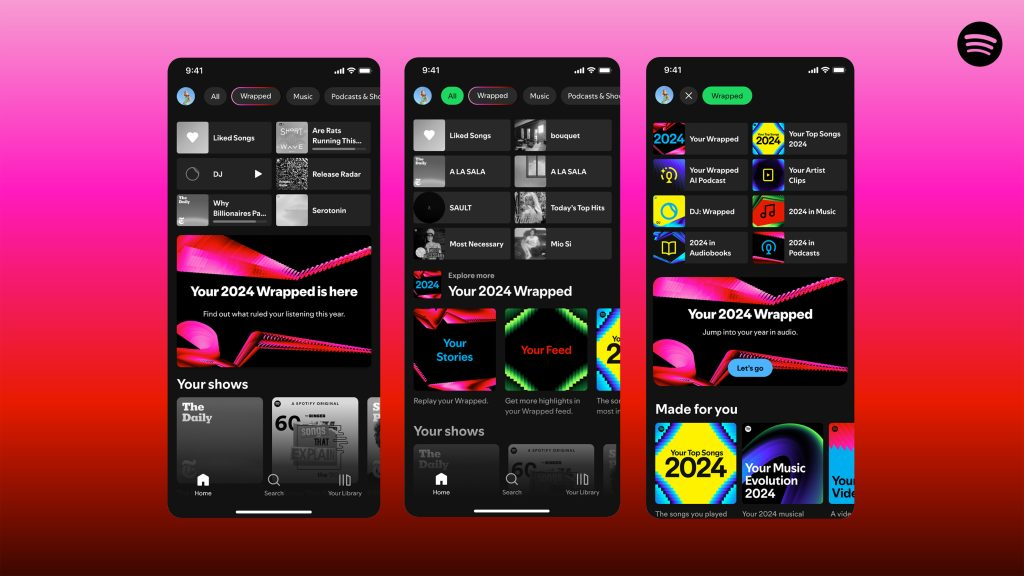
\includegraphics[width=0.5\textwidth]{../graphics/spotify_wrapped.png} % tên file hình
    \caption{Spotify Wrapped} % chú thích
    \label{fig:example} % nhãn để tham chiếu
\end{figure}

Trong suốt quá trình phát triển, Spotify đã chứng kiến và góp phần tạo nên nhiều dấu ấn lịch sử của ngành nhạc số, thay đổi thói quen thưởng thức âm nhạc của cả một thế hệ. Không chỉ là nơi phát nhạc, Spotify còn là một nền tảng truyền cảm hứng, đưa âm nhạc đến gần hơn với cuộc sống hằng ngày và khẳng định sức mạnh của công nghệ trong việc kết nối con người qua âm nhạc.\\
\subsection{Vấn đề thực tế – Nhu cầu phân tích dữ liệu Spotify (xu hướng âm nhạc, gợi ý nhạc, phân tích nghệ sĩ)}
Trong kỷ nguyên số, lượng dữ liệu âm nhạc mà Spotify quản lý và tạo ra mỗi ngày là vô cùng khổng lồ: hàng tỷ lượt nghe, tìm kiếm, thêm vào playlist, chia sẻ và tương tác xã hội. Việc phân tích dữ liệu từ Spotify không chỉ phục vụ mục tiêu thương mại mà còn mang lại nhiều giá trị trong nghiên cứu, phát triển công nghệ và thậm chí là lĩnh vực văn hóa – xã hội. Một số nhóm đối tượng tiêu biểu có nhu cầu sử dụng dữ liệu này như sau:\\
\subsubsection{Nhà nghiên cứu âm nhạc và dữ liệu}
\begin{itemize}
    \item Phân tích xu hướng nghe nhạc theo thời gian, theo khu vực địa lý hoặc theo độ tuổi.

    \item Nghiên cứu mối liên hệ giữa đặc điểm âm nhạc (tempo, energy, danceability) với mức độ phổ biến.

    \item Tạo ra các mô hình dự đoán bài hát/ nghệ sĩ có khả năng trở thành xu hướng trong tương lai.
\end{itemize}
\subsubsection{Người dùng và cộng đồng nghe nhạc:}
\begin{itemize}
    \item Khám phá thói quen nghe nhạc cá nhân và so sánh với bạn bè hoặc cộng đồng.

    \item Tìm kiếm và gợi ý playlist phù hợp với tâm trạng, bối cảnh, hoạt động hàng ngày.
    
    \item Theo dõi các bảng xếp hạng như Top 50 Global hay Top 50 theo quốc gia để nắm bắt trào lưu âm nhạc mới.
\end{itemize}

\subsubsection{Nghệ sĩ và hãng thu âm}
\begin{itemize}
    \item Phân tích dữ liệu lượt nghe để đánh giá mức độ thành công của ca khúc, album hay tour diễn.

    \item Nghiên cứu thị trường mục tiêu: quốc gia, độ tuổi, giới tính của người nghe.

    \item Tối ưu hóa chiến lược phát hành (ngày ra mắt, thể loại, hợp tác nghệ sĩ) nhằm tối đa hóa doanh thu và mức độ lan tỏa.
\end{itemize}

\subsubsection{Doanh nghiệp và tổ chức quảng cáo}
\begin{itemize}
    \item Sử dụng dữ liệu hành vi người dùng để tối ưu hóa việc phân phối quảng cáo âm thanh và banner.

    \item Xác định nhóm khách hàng tiềm năng thông qua sở thích âm nhạc, từ đó đưa ra chiến lược tiếp thị hiệu quả hơn.

    \item Tận dụng dữ liệu thời gian thực để phân tích hiệu quả chiến dịch marketing (ví dụ: chiến dịch gắn liền với sự kiện âm nhạc quốc tế).
\end{itemize}

\subsubsection{Kỹ sư dữ liệu và nhà phát triển hệ thống}
\begin{itemize}
    \item Nhu cầu xử lý big data với tốc độ cao, từ đó yêu cầu hạ tầng dữ liệu mạnh mẽ (Apache Kafka, Spark, Hadoop).

    \item Đảm bảo tính chính xác, toàn vẹn và bảo mật của dữ liệu khi có hàng trăm triệu người dùng cùng truy cập.

    \item Xây dựng pipeline phân tích dữ liệu streaming theo thời gian thực, phục vụ cho hệ thống gợi ý cá nhân hóa.
\end{itemize}

\section{Mục tiêu đồ án}

\subsection{Thu thập và tiền xử lý dữ liệu}
\begin{itemize}
    \item Thu thập các dataset về Spotify từ Kaggle, API Sportify, ReccoBeats
    \item Làm sạch và chuẩn hóa dữ liệu: xử lý giá trị thiếu, định dạng ngày, chuẩn hóa các trường thuộc tính, loại bỏ dữ liệu dư thừa.
\end{itemize}

\subsection{Thiết kế và xây dựng hệ thống dữ liệu}
\begin{itemize}
    \item Thiết kế mô hình dữ liệu quan hệ (ERD, RM) dựa trên các file CSV đã chuẩn hóa.
    \item Tổ chức dữ liệu vào hệ quản trị CSDL (MySQL,..) nhằm đảm bảo tính toàn vẹn, tối ưu truy vấn và dễ dàng mở rộng.
    \item Áp dụng các kỹ thuật Data Engineering: indexing, trigger, backup/restore, tối ưu hóa dữ liệu.
\end{itemize}

\subsection{Xây dựng pipeline xử lý và phân tích dữ liệu}
\begin{itemize}
    \item Thiết kế mô hình dữ liệu quan hệ (ERD) dựa trên các file CSV đã chuẩn hóa.
    \item Tổ chức dữ liệu vào hệ quản trị CSDL (MySQL,..) nhằm đảm bảo tính toàn vẹn, tối ưu truy vấn và dễ dàng mở rộng.
    \item Áp dụng các kỹ thuật Data Engineering: indexing, trigger, backup/restore, tối ưu hóa dữ liệu.
\end{itemize}


\subsection{Phân tích và trực quan hóa dữ liệu Spotify}
\begin{itemize}
    \item Phân tích xu hướng âm nhạc: sự nổi bật của ca khúc/nghệ sĩ, vòng đời của bài hát (Hot/Cold cycle), sự khác biệt giữa các quốc gia.
    \item Khai thác đặc trưng âm nhạc (danceability, energy, acousticness, valence, tempo, v.v.) để tìm mối liên hệ với độ phổ biến.
    \item Trực quan hóa dữ liệu qua dashboard (Streamlit/Matplotlib/Seaborn), cho phép người dùng tra cứu bảng xếp hạng, so sánh quốc gia, xem biểu đồ xu hướng.
    \item còn tìm hiểu để thay đổi hoặc mở rộng
\end{itemize}

\subsection{Ứng dụng và mở rộng}
\begin{itemize}
    \item Hỗ trợ người dùng (sinh viên, nhà nghiên cứu, nghệ sĩ, doanh nghiệp) trong việc khai thác thông tin từ dữ liệu Spotify.
    \item Đề xuất khả năng mở rộng với Machine Learning như gợi ý bài hát, dự đoán bài hát tiềm năng sẽ vào bảng xếp hạng.
    \item Nâng cấp hệ thống thành mô hình phân tích dữ liệu streaming thời gian thực (Kafka + Spark) để phục vụ cập nhật liên tục.
    \item còn tìm hiểu để thay đổi hoặc mở rộng ( chọn 1 hướng để phát triển)
\end{itemize}






\section{Tìm hiểu và phân tích đặc điểm của nguồn dữ liệu}
Trong quá trình thực hiện đề tài, nhóm đã tiến hành khảo sát và lựa chọn các nguồn dữ liệu 
liên quan trực tiếp đến lĩnh vực nghiên cứu. 
Mỗi nguồn dữ liệu đều có những đặc trưng riêng về cấu trúc, dung lượng, cũng như mức độ phù hợp 
với yêu cầu của bài toán. 
Việc phân tích đặc điểm của từng nguồn giúp nhóm:
\begin{itemize}
    \item Đánh giá tính tin cậy và độ bao phủ của dữ liệu.
    \item Hiểu rõ cấu trúc, định dạng, và mối quan hệ giữa các thuộc tính.
    \item Xác định những vấn đề cần tiền xử lý (dữ liệu thiếu, dữ liệu nhiễu, trùng lặp, …).
    \item Đề ra phương án tích hợp và khai thác hiệu quả cho hệ thống.
\end{itemize}

\large{Dưới đây là phân tích chi tiết từng nguồn dữ liệu mà nhóm sử dụng :}

\subsection{Nguồn 1: Spotify Top 50 Playlist Songs }

\begin{itemize}
    \item     \textbf{Link dataset: }https://www.kaggle.com/datasets/anxods/spotify-top-50-playlist-songs-anxods
    \item     \textbf{Link github: }https://github.com/minhnhut273/spotify-data-project
\end{itemize}

\subsubsection{Giới thiệu dữ liệu}
  \textbf{Tổng quan} 


    - Bộ dữ liệu cung cấp thông tin bài hát nằm trong bảng xếp hạng Top 50 của Spotify của một số quốc gia gồm 9 nước (United States, Spain, United Kingdom, Italy, France, Mexico, Argentina, Japan, South Korea) và 1 bảng xếp hạng chung top 50 trên thế giới.

  
    - Phạm vi dữ liệu ngoài vị trí địa lý còn về mặt thời gian bộ dataset cung cấp nằm trong khoảng 05/2023 đến 11/2024.

   \textbf{Một số đặc trựng ban đầu:}

\begin{itemize}
    \item \textbf{date}: Ngày thu thập dữ liệu hoặc ngày xếp hạng. 


    \item \textbf{position}: Vị trí của bài hát trong bảng xếp hạng Top 50. 


    \item \textbf{song}: Tên bài hát. 


    \item \textbf{artist}: Tên nghệ sĩ hoặc nhóm nghệ sĩ chính. 


    \item \textbf{popularity}: Chỉ số phổ biến (Spotify popularity score, 0–100). 


    \item \textbf{duration\_ms}: Độ dài bài hát tính bằng mili-giây. 


    \item \textbf{album\_type}: Loại album chứa track này (ví dụ: album, single, compilation). 


    \item \textbf{total\_tracks}: Tổng số track trong album chứa bài hát đó. 


    \item \textbf{release\_date}: Ngày phát hành album (chứa bài hát này).

    \item \textbf{is\_explicit}: Cho biết bài hát có nội dung 18+ hay không. 
   

    \item \textbf{album\_cover\_url}: Link ảnh bìa album.
\end{itemize}

\begin{figure}[h] % môi trường figure để quản lý hình
    \centering % căn giữa
    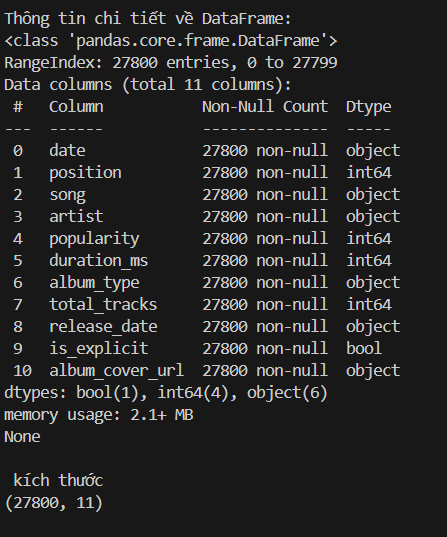
\includegraphics[width=0.5\textwidth]{../graphics/data_top50/raw.png} % tên file hình
    \caption{Đặc điểm chung của các dataset} % chú thích
    \label{fig:example} % nhãn để tham chiếu
\end{figure}
\textbf{=> Kết quả có được 10 file spotify-streaming-top-50-{region}.csv có đặc điểm như hình trên}

 \subsubsection{Bổ sung dữ liệu:}

 \textbf{- Dùng Spotify API để hoàn thiện metadata}
 \\ 
 \begin{itemize}
     \item \textbf{Giới thiệu API:} Spotify Web API là dịch vụ do Spotify cung cấp. Cho phép lập trình viên truy cập dữ liệu nhạc số trên Spotify, hoạt động qua HTTP request (RESTful API). 
     \item \textbf{Mục đích:} Do nhóm nhận thấy các trường dữ liệu của dataset gốc chưa cung cấp đầy đủ, chi tiết về metadata của dữ liệu nên nhóm quyết định sử dụng API này để hoàn thiện nó.
     \item \textbf{Các trường có thể thêm gồm:}
    \begin{itemize}
        \item \textbf{track\_id}: ID duy nhất của bài hát trên Spotify.
        \item \textbf{album\_id}: ID duy nhất của album chứa bài hát.
        \item \textbf{uri}: Định danh Spotify URI (dùng để mở trực tiếp trong Spotify).
        \item \textbf{href}: Link API đến resource (track/album) trong Spotify Web API.
        \item \textbf{external\_url}: Link mở trên Spotify (dành cho người dùng).
        \item \textbf{external\_ids}: Thông tin định danh khác (ví dụ ISRC – mã nhận dạng bản ghi).
        \item \textbf{disc\_number}: Số đĩa (trong trường hợp album nhiều đĩa).
        \item \textbf{track\_number}: Vị trí bài hát trong album/đĩa.
        \item \textbf{release\_date\_precision}: Độ chính xác của ngày phát hành (có thể là year, month, hoặc day).
        \item \textbf{is\_playable}: Cho biết bài hát có thể phát được không (True/False).
        \item \textbf{linked\_from}: Nếu bài hát được liên kết từ một track khác (ví dụ bản sao trong album khác).
        \item \textbf{preview\_url}: Link nghe thử 30 giây bài hát.
        \item \textbf{restrictions}: Các giới hạn (ví dụ chỉ phát được ở một số quốc gia).
        \item \textbf{available\_markets}: Danh sách quốc gia mà track này có sẵn.
        \item \textbf{genres}: Thể loại âm nhạc nghệ sĩ theo đuổi.
    \end{itemize}
 \end{itemize}
 
\begin{figure}[h] % môi trường figure để quản lý hình
    \centering % căn giữa
    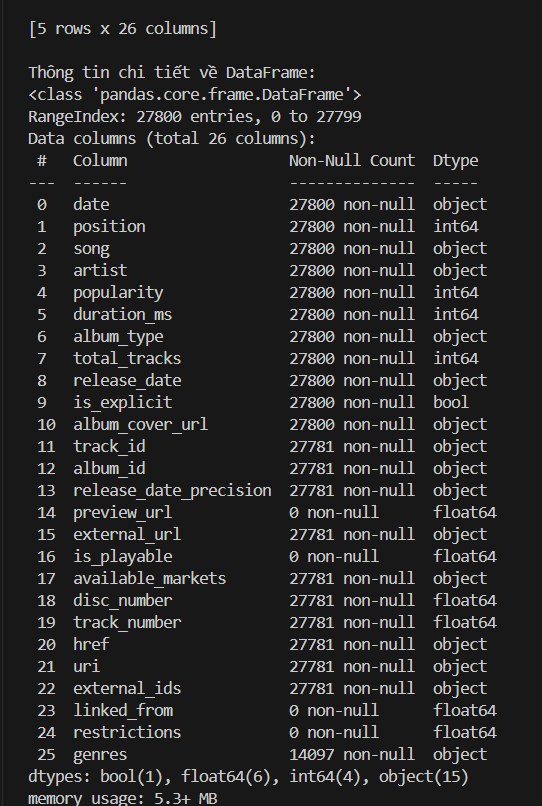
\includegraphics[width=0.5\textwidth]{../graphics/data_top50/figure/script/raw_meta/Screenshot 2025-09-30 225603.png} % tên file hình
    \caption{Các trường sau khi thêm} % chú thích
    \label{fig:example} % nhãn để tham chiếu
\end{figure}

\textbf{=> Kết quả có được các file ..with-meta.csv có đặc điểm như hình trên}

\begin{itemize}
    \item \textbf{Hạn chế:} Tuy nhiên, do một số chính sách mới ra cuối năm 2024 của Spotify dẫn đến các nhóm người không thể truy cập được một số nội dung ( chart, lyric,...) trong đó có audio feature - nguồn dữ liệu mà nhóm quan tâm.
\end{itemize}
\textbf{- Dùng ReccoBeats để bổ sung audio feature: }
\begin{itemize}
    \item \textbf{Giới thiệu API:}Recobeats API là một dịch vụ bên thứ ba giúp lấy dữ liệu nhạc từ Spotify (playlist, audio features, metadata) và dùng cho phân tích hoặc gợi ý nhạc. Tuy nhiên nó không phải API chính thức.
    
    % , nên có thể bị giới hạn hoặc phụ thuộc vào quyền truy cập Spotify. 
    \item \textbf{Các trường có thể thêm: }
    \begin{itemize}
    \item \textbf{href}: Link Spotify đến bài hát (https://open.spotify.com/track/<track\_id>). Dùng để mở hoặc kiểm tra thủ công.
    \item \textbf{acousticness}: Mức độ “mộc” (0.0–1.0). Cao => nhạc acoustic, ít electronic.
    \item \textbf{danceability}: Độ dễ nhảy (0.0–1.0). Cao => dễ nhảy, dựa trên nhịp, groove, tempo.
    \item \textbf{energy}: Cường độ/độ bốc (0.0–1.0). Liên quan tới tempo, loudness, mật độ âm thanh.
    \item \textbf{instrumentalness}: Khả năng không lời (0.0–1.0). >0.5 thường là nhạc cụ/không lời.
    \item \textbf{key}: Tông nhạc (0–11, -1 nếu không phát hiện). Ví dụ: 0=C, 1=C\#/Db, … 11=B. 
    \item \textbf{liveness}: Dấu hiệu biểu diễn live (0.0–1.0). >0.8 thường là bản live.
    \item \textbf{loudness}: Độ ồn trung bình (dB, -60 => 0). Giá trị càng gần 0 càng to. 
    \item \textbf{mode}: Điệu thức: 1 = Major (tươi sáng), 0 = Minor (trầm buồn). 
    \item \textbf{speechiness}: Tỷ lệ lời nói (0.0–1.0). >0.66: chủ yếu là nói; 0.33–0.66: rap/spoken; <0.33: chủ yếu là nhạc.
    \item \textbf{tempo}: Nhịp độ (BPM, 0–250). Nhạc phổ biến: 60–200 BPM.
    \item \textbf{valence}: Độ “tươi vui”/tích cực (0.0–1.0). 0.0 = buồn/tối, 1.0 = vui/sáng.
    \end{itemize}

\end{itemize}

\begin{figure}[h] % môi trường figure để quản lý hình
    \centering % căn giữa
    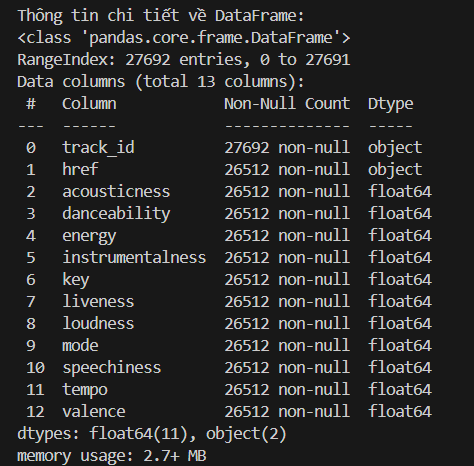
\includegraphics[width=0.5\textwidth]{../graphics/data_top50/figure/script/raw_audio/Screenshot 2025-09-30 230213.png} % tên file hình
    \caption{Bảng đặc trưng} % chú thích
    \label{fig:example} % nhãn để tham chiếu
\end{figure}

    \textbf{=> Kết quả có các file ..with-audio.csv có đặc điểm như hình trên}








% \subsubsection{Tiền xử lý }

% \textbf{- Xử lí Metadata: }

% \begin{itemize}
%     \item \textbf{Giữ lại một số trường  cần thiết:}
      
% \begin{itemize}

%     % Giữ lại một số trường cần thiết:
%     \begin{itemize}
%         \item \textbf{date}  phân tích theo thời gian.
%         \item \textbf{position} => vị trí xếp hạng trong Top 50.
%         \item \textbf{song} => tên bài hát.
%         \item \textbf{artist} => tên nghệ sĩ.
%         \item \textbf{track\_id} => khóa chính để join với with-audio.
%         \item \textbf{popularity} => đo mức độ phổ biến.
%         \item \textbf{duration\_ms} => độ dài bài hát (có thể phân tích thêm).
%         \item \textbf{is\_explicit} => xem tỷ lệ nhạc explicit.
%         \item \textbf{album\_id} => phân tích theo album (nếu cần).
%         \item \textbf{release\_date} => phân tích mới/cũ.
%         \item \textbf{genres} => phân tích xu hướng thể loại.
%     \end{itemize}

%     % Bỏ các trường không cần thiết:
%     \item \textbf{Bỏ:}
%     \begin{itemize}
%         \item \textbf{album\_type}, \textbf{total\_tracks} => chỉ mô tả album.
%         \item \textbf{release\_date\_precision} => nếu không phân tích độ chính xác ngày phát hành.
%         \item \textbf{album\_cover\_url}, \textbf{preview\_url}, \textbf{external\_url}, \textbf{uri}, \textbf{href}, \textbf{external\_ids} => chỉ để hiển thị/mở nhạc.
%         \item \textbf{is\_playable}, \textbf{available\_markets}, \textbf{disc\_number}, \textbf{track\_number}, \textbf{linked\_from}, \textbf{restrictions}  không cần cho phân tích.
%     \end{itemize}

% \end{itemize}
% \end{itemize}
% \begin{itemize}
%     \item  \textbf{Xử lý Missing Values (Data Cleaning)}
%     \begin{itemize}
%         \item \textbf{Mục tiêu:} đảm bảo dữ liệu không còn NaN ở các cột quan trọng.
%         \item \texttt{track\_id:} nếu thiếu => điền \texttt{"unknown\_track"} (không xóa để giữ dữ liệu phân tích).
%         \item \texttt{album\_id:} nếu thiếu => \texttt{"unknown\_album"}.
%         \item \texttt{release\_date:}
%         \begin{itemize}
%             \item Nếu chỉ có năm => ghép \texttt{"YYYY-01-01"}.
%             \item Nếu NaN => cũng dùng \texttt{"YYYY-01-01"} dựa trên năm nhỏ nhất trong cột \texttt{date}.
%         \end{itemize}
%         \item \texttt{genres:} nếu NaN => \texttt{"unknown"}.
%         \item \textbf{ Kết quả:} file mới không còn dòng NaN cho \texttt{track\_id}, \texttt{album\_id}, \texttt{release\_date}, \texttt{genres}.
%     \end{itemize}

%     \item  \textbf{Chuẩn hóa dữ liệu (Standardization)}
%     \begin{itemize}
%         \item \textbf{Mục tiêu:} đưa dữ liệu về format thống nhất để dễ phân tích.
%         \item \texttt{date \& release\_date:}
%         \begin{itemize}
%             \item Convert toàn bộ sang \texttt{datetime} (YYYY-MM-DD).
%         \end{itemize}
%         \item \texttt{genres:}
%         \begin{itemize}
%             \item Nếu nhiều genre => lấy genre đầu tiên làm \texttt{main\_genre}.
%         \end{itemize}
%         \item \texttt{is\_explicit:} Convert về 0/1 (boolean => int).
%         \item \texttt{duration\_ms:} giữ nguyên, chưa cần chia phút/giây.
%         \item \texttt{song, artist:} giữ nguyên, chưa chuẩn hóa.
%         \item \textbf{ Kết quả:} file chuẩn hóa có \texttt{date}, \texttt{release\_date} đúng kiểu ngày, 
%         \texttt{is\_explicit} đồng nhất 0/1, \texttt{main\_genre} rõ ràng cho phân tích.
%     \end{itemize}
% \end{itemize}
%      \textbf{=> Kết quả có được file ..with-meta-clean.csv ở các floder}
    

% \begin{figure}[h] % môi trường figure để quản lý hình
%     \centering % căn giữa
%     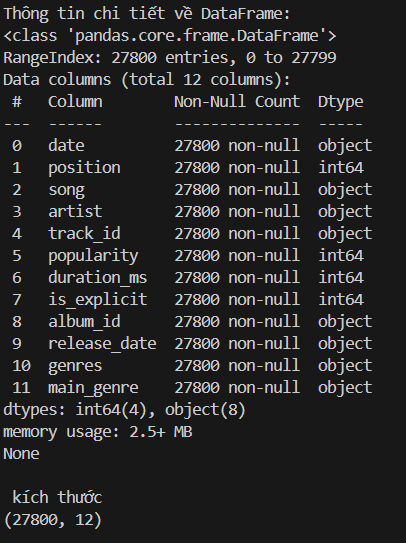
\includegraphics[width=0.5\textwidth]{../graphics/data_top50/figure/script/meta_clean_1/Screenshot 2025-10-02 191458.png} % tên file hình
%     \caption{File meta-clean} % chú thích
%     \label{File meta-clean} % nhãn để tham chiếu
% \end{figure}
% \clearpage


% \textbf{-Xử lí file audio}
% \begin{itemize}
%     \item  \textbf{Bước 1. Kiểm tra \& xử lý Missing Values}
%     \begin{itemize}
%         \item \texttt{track\_id, href:} giữ nguyên (định danh và link).
%         \item \textbf{Các đặc trưng [0–1]} (\texttt{danceability, energy, valence, acousticness, instrumentalness, liveness, speechiness}):
%         \begin{itemize}
%             \item Nếu NaN => thay bằng \textit{median} (hoặc giá trị phổ biến nhất).
%             \item Sau đó clip về \([0,1]\).
%         \end{itemize}
%         \item \texttt{tempo:} 
%         \begin{itemize}
%             \item Nếu NaN hoặc bất thường (\(<30\) hoặc \(>250\)) => thay bằng median.
%         \end{itemize}
%         \item \texttt{loudness:}
%         \begin{itemize}
%             \item Nếu NaN hoặc bất thường (\(<-60\) hoặc \(>0\)) => thay bằng median.
%         \end{itemize}
%         \item \texttt{mode (0/1):} nếu NaN => điền bằng giá trị chiếm đa số trong cột.
%         \item \texttt{key:} 
%         \begin{itemize}
%             \item Nếu \(-1\) hoặc NaN => thay bằng giá trị gần nhất (forward/backward fill hoặc mode).
%             \item Sau đó map sang tên nốt nhạc.
%         \end{itemize}
%     \end{itemize}

%     \item  \textbf{Bước 2. Chuẩn hóa dữ liệu (Standardization)}
%     \begin{itemize}
%         \item \textbf{Các đặc trưng [0–1]} (\texttt{danceability, energy, valence, acousticness, instrumentalness, liveness, speechiness}):
%         \begin{itemize}
%             \item Clip về \([0,1]\), giữ nguyên cột gốc (không thêm).
%         \end{itemize}
%         \item \texttt{tempo:}
%         \begin{itemize}
%             \item Giữ nguyên cột gốc.
%             \item Thêm \texttt{tempo\_norm = (tempo - 30)/(250-30)}.
%         \end{itemize}
%         \item \texttt{loudness:}
%         \begin{itemize}
%             \item Giữ nguyên cột gốc.
%             \item Thêm \texttt{loudness\_norm = (loudness + 60)/60}.
%         \end{itemize}
%         \item \texttt{mode:} giữ nguyên 0/1 (NaN đã được thay).
%         \item \texttt{key:}
%         \begin{itemize}
%             \item Giữ nguyên cột \texttt{key}.
%             \item Thêm cột mới \texttt{key\_name} (C, C\#, D, …, B).
%             \item Đảm bảo không còn \texttt{"unknown"} (đã thay bằng giá trị hợp lệ).
%         \end{itemize}
%     \end{itemize}

%     \item  \textbf{Cột mới sau xử lý:}
%     \begin{itemize}
%         \item \texttt{tempo\_norm} => tempo chuẩn hóa [0,1].
%         \item \texttt{loudness\_norm} => loudness chuẩn hóa [0,1].
%         \item \texttt{key\_name} => tên nốt nhạc thay vì số.
%     \end{itemize}
% \end{itemize}
% \textbf{=> Kết quả ghi đè vào các file ..with-audio.csv}
% \\
%  \begin{figure}[h] % môi trường figure để quản lý hình
%     \centering % căn giữa
%     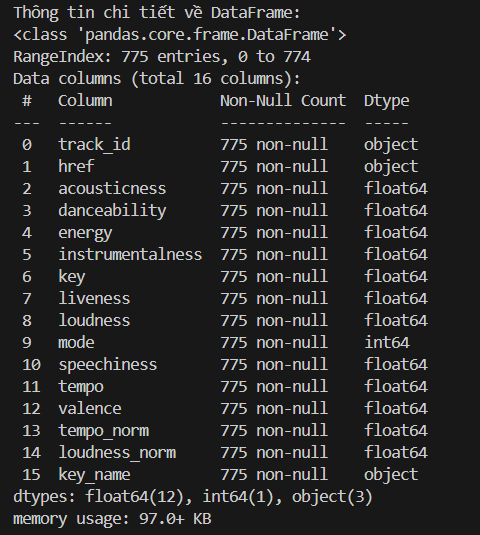
\includegraphics[width=0.75\textwidth]{../graphics/data_top50/figure/script/Screenshot 2025-10-02 192420.png} % tên file hình
%     \caption{File meta-clean} % chú thích
%     \label{File meta-clean} % nhãn để tham chiếu
% \end{figure}
% \clearpage


\subsubsection{Tiền xử lý}

\textbf{- Xử lý Metadata:}

\begin{itemize}
    \item \textbf{Giữ lại một số trường cần thiết:}
    \begin{itemize}
        \item \textbf{date} — phân tích theo thời gian.
        \item \textbf{position} — vị trí xếp hạng trong Top 50.
        \item \textbf{song} — tên bài hát.
        \item \textbf{artist} — tên nghệ sĩ.
        \item \textbf{track\_id} — khóa chính để join với with-audio.
        \item \textbf{popularity} — đo mức độ phổ biến.
        \item \textbf{duration\_ms} — độ dài bài hát (có thể phân tích thêm).
        \item \textbf{is\_explicit} — xem tỷ lệ nhạc explicit.
        \item \textbf{album\_id} — phân tích theo album (nếu cần).
        \item \textbf{release\_date} — phân tích bài mới/cũ.
        \item \textbf{genres} — phân tích xu hướng thể loại.
        \item \textbf{Bỏ các trường không cần thiết còn lại}
    \end{itemize}

    
    % \begin{itemize}
    %     \item \textbf{album\_type}, \textbf{total\_tracks} 
    %     \item \textbf{release\_date\_precision} — nếu không cần độ chính xác ngày phát hành.
    %     \item \textbf{album\_cover\_url}, \textbf{preview\_url}, \textbf{external\_url}, \textbf{uri}, \textbf{href}, \textbf{external\_ids} — chỉ để hiển thị/mở nhạc.
    %     \item \textbf{is\_playable}, \textbf{available\_markets}, \textbf{disc\_number}, \textbf{track\_number}, \textbf{linked\_from}, \textbf{restrictions} — không cần cho phân tích.
    % \end{itemize}
\end{itemize}

\begin{itemize}
    \item \textbf{Xử lý Missing Values (Data Cleaning):}
    \begin{itemize}
        \item \textbf{Mục tiêu:} đảm bảo dữ liệu không còn NaN ở các cột quan trọng.
        \item \texttt{track\_id}, exttt{album\_id} và \texttt{genres} : nếu thiếu $\rightarrow$ điền \texttt{"unknown\_track"}, \texttt{"unknown\_album"} và \texttt{"unknown"}.
        \item \texttt{release\_date:}
        \begin{itemize}
            \item Nếu chỉ có năm $\rightarrow$ ghép \texttt{"YYYY-01-01"}.
            \item Nếu NaN $\rightarrow$ dùng \texttt{"YYYY-01-01"} dựa trên năm nhỏ nhất trong cột \texttt{date}.
        \end{itemize}

    \end{itemize}

    \item \textbf{Chuẩn hóa dữ liệu (Standardization):}
    

    

    \begin{itemize}
        \item \textbf{Mục tiêu:} đưa dữ liệu về format thống nhất để dễ phân tích.
        \item \texttt{date} \& \texttt{release\_date:}
        \begin{itemize}
            \item Convert toàn bộ sang \texttt{datetime} (YYYY-MM-DD).
        \end{itemize}
        \item \texttt{genres:}
        \begin{itemize}
            \item Nếu có nhiều genre $\rightarrow$ lấy genre đầu tiên tạo cột \texttt{main\_genre}.
        \end{itemize}
        \item \texttt{is\_explicit:} convert về 0/1 (boolean $\rightarrow$ int).
        % \item \texttt{duration\_ms:} giữ nguyên (chưa chia phút/giây).
        % \item \texttt{song, artist:} giữ nguyên, chưa chuẩn hóa.
        % \item \textbf{Kết quả:} file chuẩn hóa có \texttt{date}, \texttt{release\_date} đúng kiểu ngày, 
        % \texttt{is\_explicit} đồng nhất 0/1, \texttt{main\_genre} rõ ràng cho phân tích.
    \end{itemize}
\end{itemize}




% \begin{center}
% \vspace{0.5em}
% \textbf{=> Kết quả:} tạo được các file \texttt{...with-meta-clean.csv} có đặc điểm như hình trên.
% \end{center}


\par\vspace{1em}
\noindent\textbf{=> Kết quả:} tạo được các file \texttt{...with-meta-clean.csv} .

\clearpage
\textbf{- Xử lý file audio:}

\begin{itemize}
    \item \textbf{Bước 1. Kiểm tra \& xử lý Missing Values:}
    \begin{itemize}
        \item \texttt{track\_id, href}: giữ nguyên (định danh và link).
        \item \textbf{Các đặc trưng [0–1]} (\texttt{danceability, energy, valence, acousticness, instrumentalness, liveness, speechiness}):
        \begin{itemize}
            \item Nếu NaN $\rightarrow$ thay bằng \textit{median} (hoặc giá trị phổ biến nhất).
            \item Sau đó clip về [0,1].
        \end{itemize}
        \item \texttt{tempo:}
        \begin{itemize}
            \item Nếu NaN hoặc bất thường ($<30$ hoặc $>250$) $\rightarrow$ thay bằng median.
        \end{itemize}
        \item \texttt{loudness:}
        \begin{itemize}
            \item Nếu NaN hoặc bất thường ($<-60$ hoặc $>0$) $\rightarrow$ thay bằng median.
        \end{itemize}
        \item \texttt{mode (0/1):} nếu NaN $\rightarrow$ điền giá trị chiếm đa số trong cột.
        \item \texttt{key:}
        \begin{itemize}
            \item Nếu -1 hoặc NaN $\rightarrow$ thay bằng giá trị gần nhất (forward/backward fill hoặc mode).
           
        \end{itemize}
    \end{itemize}

    \item \textbf{Bước 2. Chuẩn hóa dữ liệu (Standardization):}
    

    
    \begin{itemize}
        \item \textbf{Các đặc trưng [0–1]} (\texttt{danceability, energy, valence, acousticness, instrumentalness, liveness, speechiness}):
        \begin{itemize}
            \item Clip về [0,1], giữ nguyên cột gốc (không thêm).
        \end{itemize}
        \item \texttt{tempo:}
        \begin{itemize}
            \item Thêm \texttt{tempo\_norm = (tempo - 30)/(250 - 30)}.
        \end{itemize}
        \item \texttt{loudness:}
        \begin{itemize}
            \item Thêm \texttt{loudness\_norm = (loudness + 60)/60}.
        \end{itemize}
        \item \texttt{key:}
        \begin{itemize}
            \item Thêm cột mới \texttt{key\_name} (C, C\#, D, …, B) và Đảm bảo không còn \texttt{"unknown"} (đã thay bằng giá trị hợp lệ).
        
        \end{itemize}
    \end{itemize}


\end{itemize}

\begin{figure}[h] % môi trường figure để quản lý hình
    \centering % căn giữa
    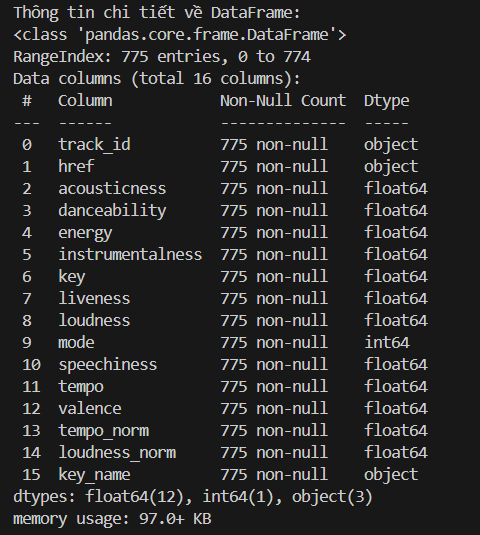
\includegraphics[width=0.75\textwidth]{../graphics/data_top50/figure/script/Screenshot 2025-10-02 192420.png} % tên file hình
    \caption{Đặc trưng chung} % chú thích
    \label{File meta-clean} % nhãn để tham chiếu
\end{figure}


\textbf{=> Kết quả:} ghi đè vào các file \texttt{...with-audio.csv} với các đặc trưng như trên.




\clearpage

















































\subsubsection{Phân tích và tìm insight:}
\begin{flushleft}
    

   
\textbf{-Công cụ khám phá: } Jupyter Notebook
\\

% \textbf{-Phân chia: } Do nguồn dataset khá lớn nên nhóm quyết định phân chia các bảng notebook thành các cụm đại diện thành các vùng dựa trên vị trí địa lý:
 
\end{flushleft}



% \begin{itemize}
%     \item \textbf{Châu Âu - Erope :} gồm italy, UK, france, spain
%     \item  \textbf{Châu Mỹ - America :} gồm argentina, usa , mexico
%     \item \textbf{Châu Á - Asia :} gồm south korea, japan
% \end{itemize}



\textbf{1. Bức tranh toàn diện về vòng đời âm nhạc trên BXH}
\begin{itemize}
    \item \textbf{1.1 Số bài hát mới phát hành theo năm}


    \begin{figure}[H]
        \centering
        % Dòng 1
        \begin{minipage}{0.45\textwidth}
            \centering
            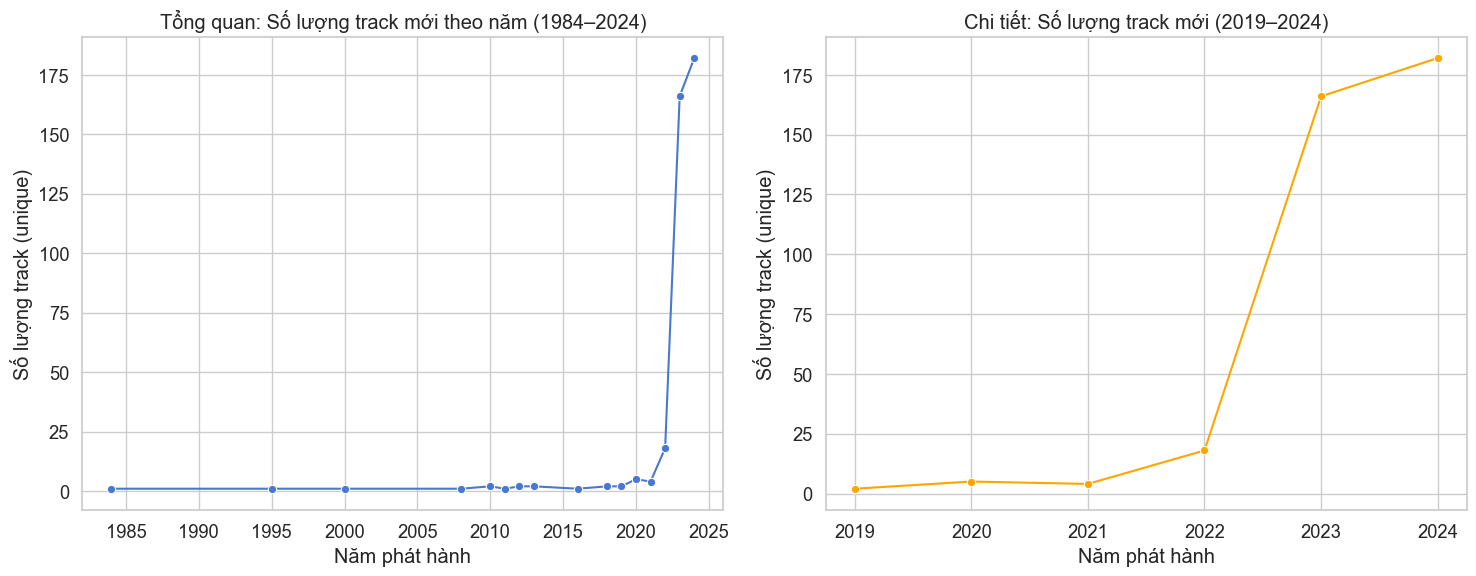
\includegraphics[width=\linewidth]{../graphics/data_top50/figure/10/EDA_argentina.png}
            \\[4pt] {\small \textbf{Argentina}}
        \end{minipage}
        \hfill
        \begin{minipage}{0.45\textwidth}
            \centering
            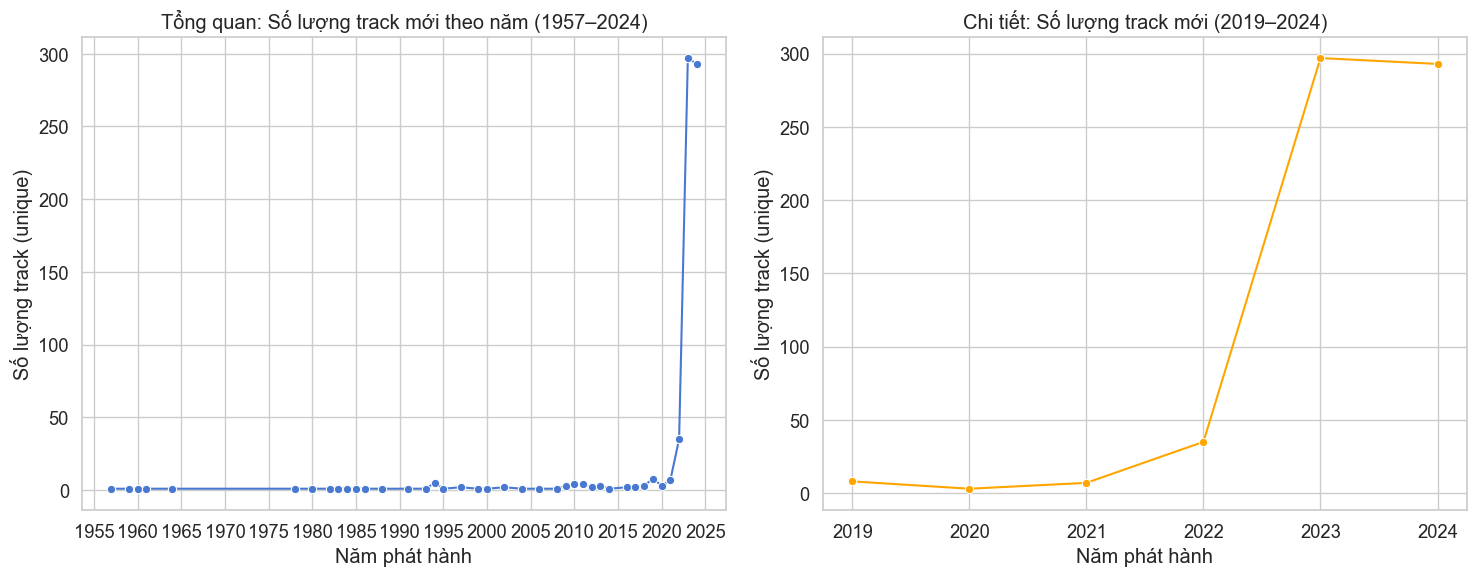
\includegraphics[width=\linewidth]{../graphics/data_top50/figure/10/EDA_france.png}
            \\[4pt] {\small \textbf{France}}
        \end{minipage}

        \vspace{0.4cm}

        % Dòng 2
        \begin{minipage}{0.45\textwidth}
            \centering
            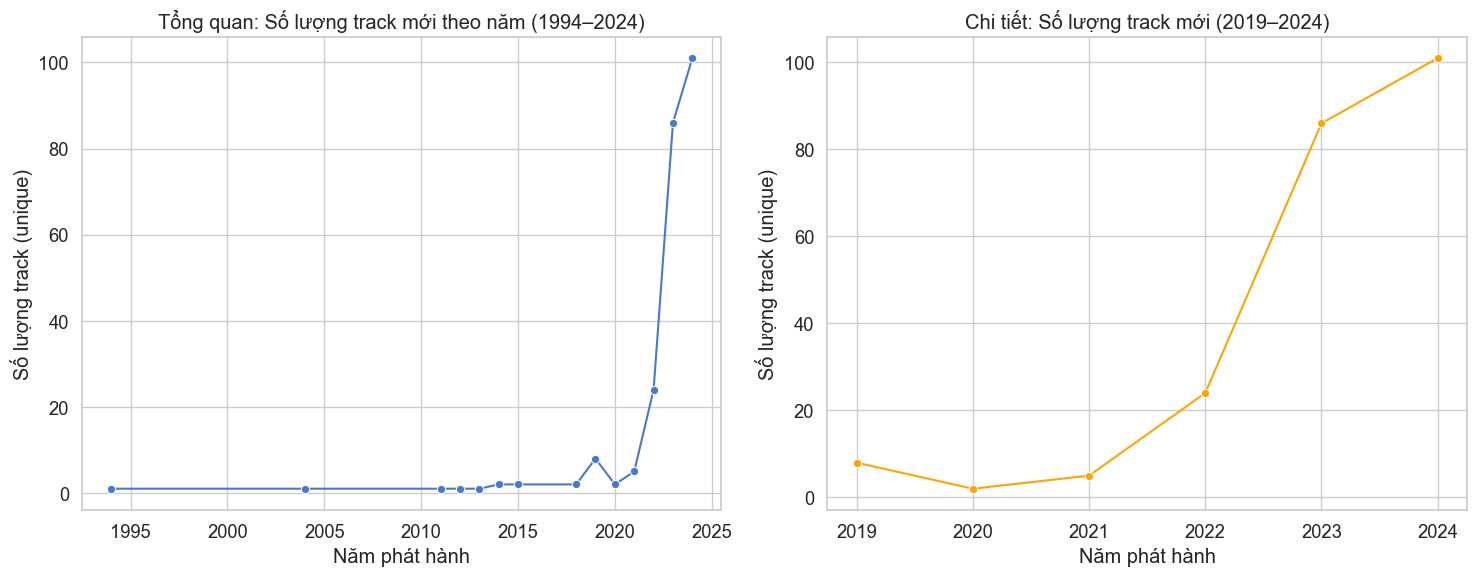
\includegraphics[width=\linewidth]{../graphics/data_top50/figure/10/EDA_japan.png}
            \\[4pt] {\small \textbf{Japan}}
        \end{minipage}
        \hfill
        \begin{minipage}{0.45\textwidth}
            \centering
            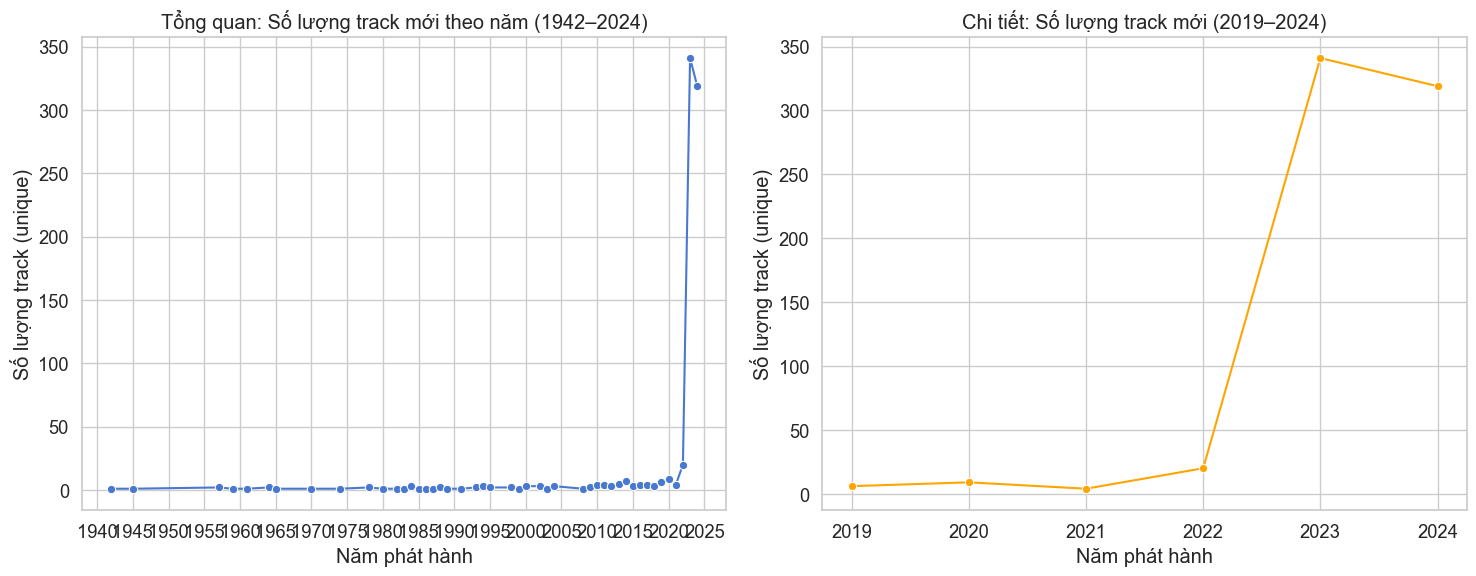
\includegraphics[width=\linewidth]{../graphics/data_top50/figure/10/EDA_world.png}
            \\[4pt] {\small \textbf{World}}
        \end{minipage}

        \caption{Track mới phát hành theo năm}
        \label{fig:energy-regions}
    \end{figure}
    
           \begin{itemize}
               \item \textbf{ Kết luận: }
               \item Trước năm 2015: số lượng track mới trên BXH rất ít, tăng trưởng chậm
               \item Giai đoạn 2015–2020: bắt đầu có xu hướng tăng nhưng chưa bùng nổ.
               \item Từ 2020 trở đi: số lượng track mới tăng vọt, đặc biệt 2023–2024 đạt đỉnh. Xuất hiện ở hầu hết quốc gia, mạnh nhất tại Mỹ \&\ Argentina, trong khi Hàn Quốc và Nhật Bản nổi bật nhờ K-pop và J-pop.
               \item Streaming và toàn cầu hoá đã tạo ra “làn sóng bùng nổ” sản xuất nhạc mới sau 2020
           \end{itemize}


    \item \textbf{1.2 Tuối thọ bài hát trên bảng xếp hạng:}



    \begin{figure}[H]
        \centering
        % Dòng 1
        \begin{minipage}{0.45\textwidth}
            \centering
            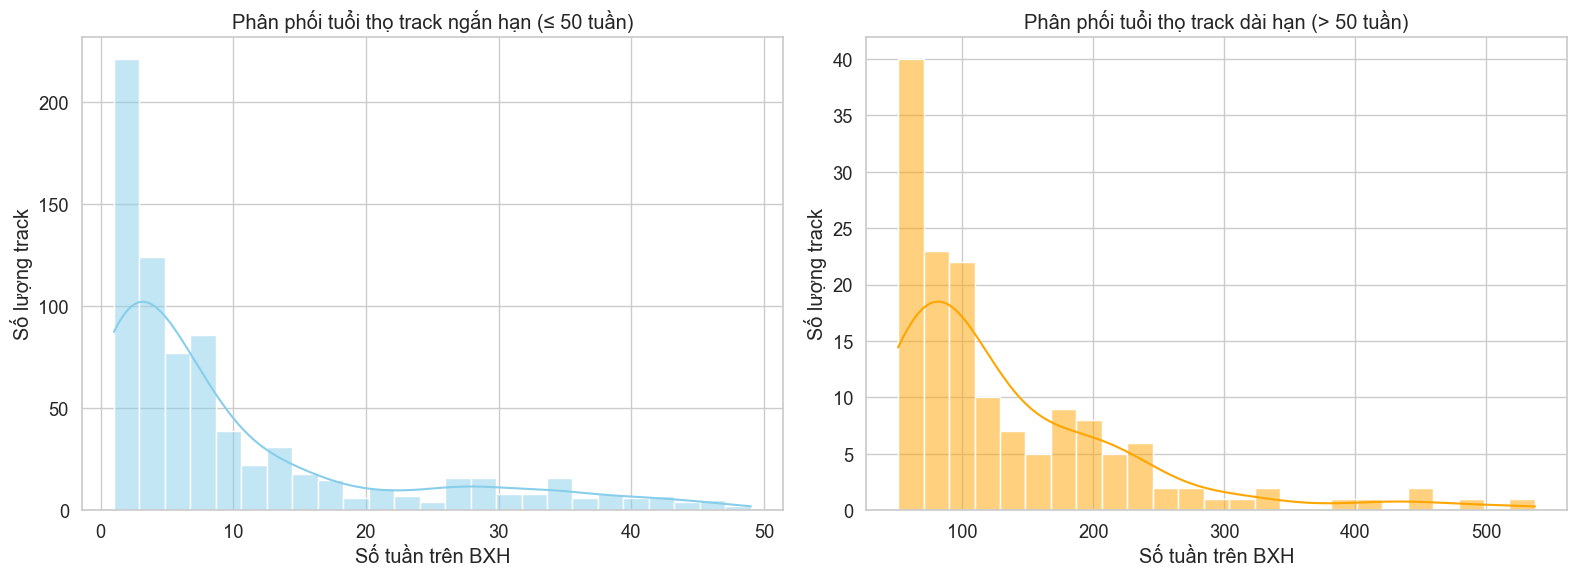
\includegraphics[width=\linewidth]{../graphics/data_top50/figure/11/EDA_usa.png}
            \\[4pt] {\small \textbf{USA}}
        \end{minipage}
        \hfill
        \begin{minipage}{0.45\textwidth}
            \centering
            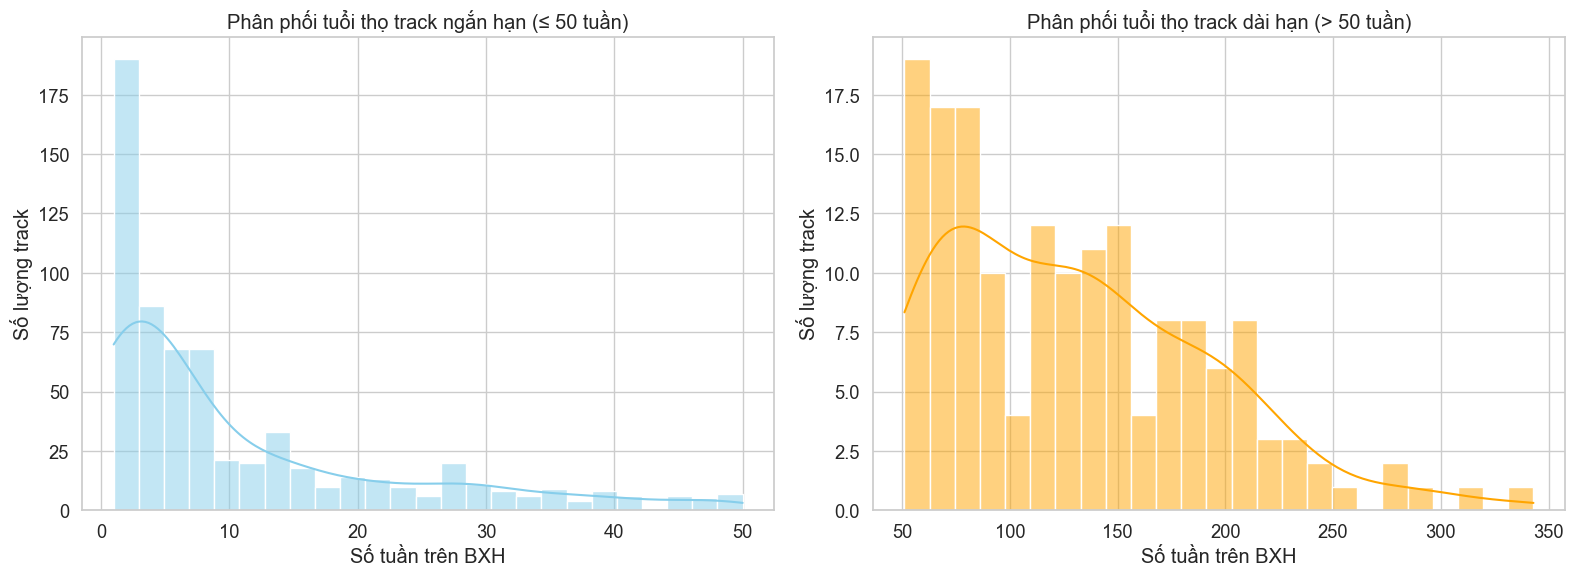
\includegraphics[width=\linewidth]{../graphics/data_top50/figure/11/EDA_italy.png}
            \\[4pt] {\small \textbf{Italy}}
        \end{minipage}

        \vspace{0.4cm}

        % Dòng 2
        \begin{minipage}{0.45\textwidth}
            \centering
            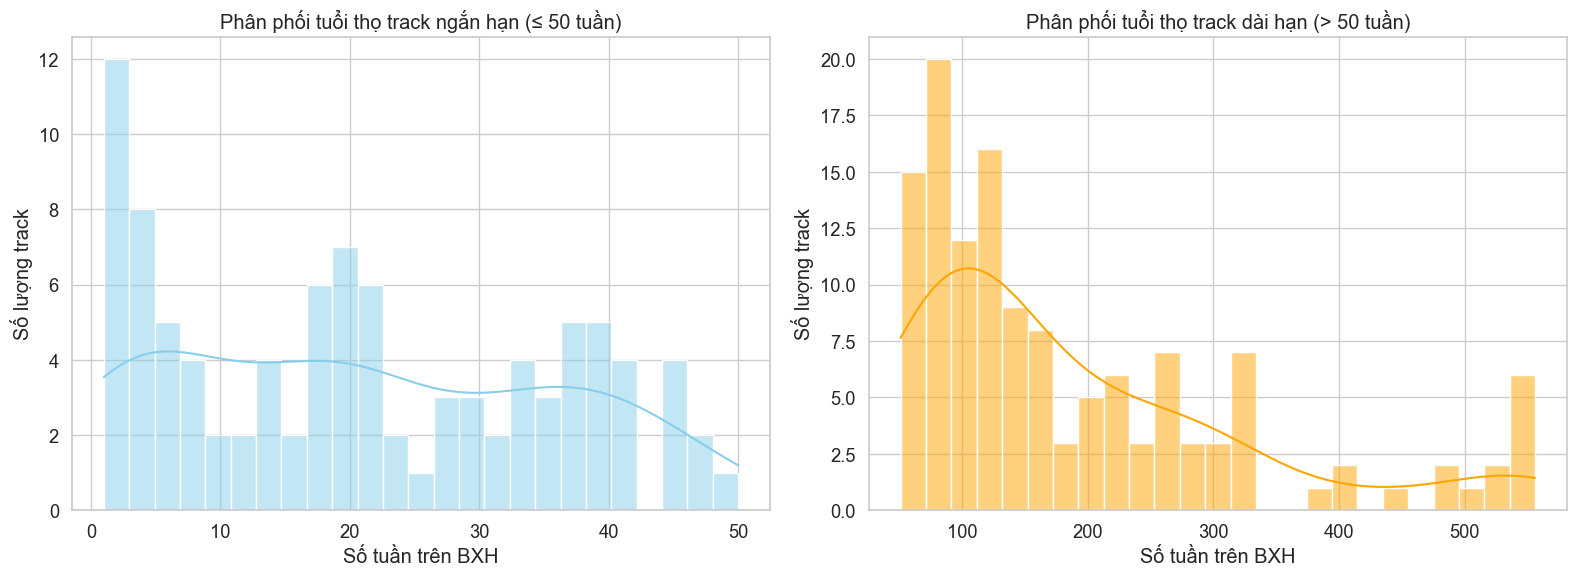
\includegraphics[width=\linewidth]{../graphics/data_top50/figure/11/EDA_japan.png}
            \\[4pt] {\small \textbf{Japan}}
        \end{minipage}
        \hfill
        \begin{minipage}{0.45\textwidth}
            \centering
            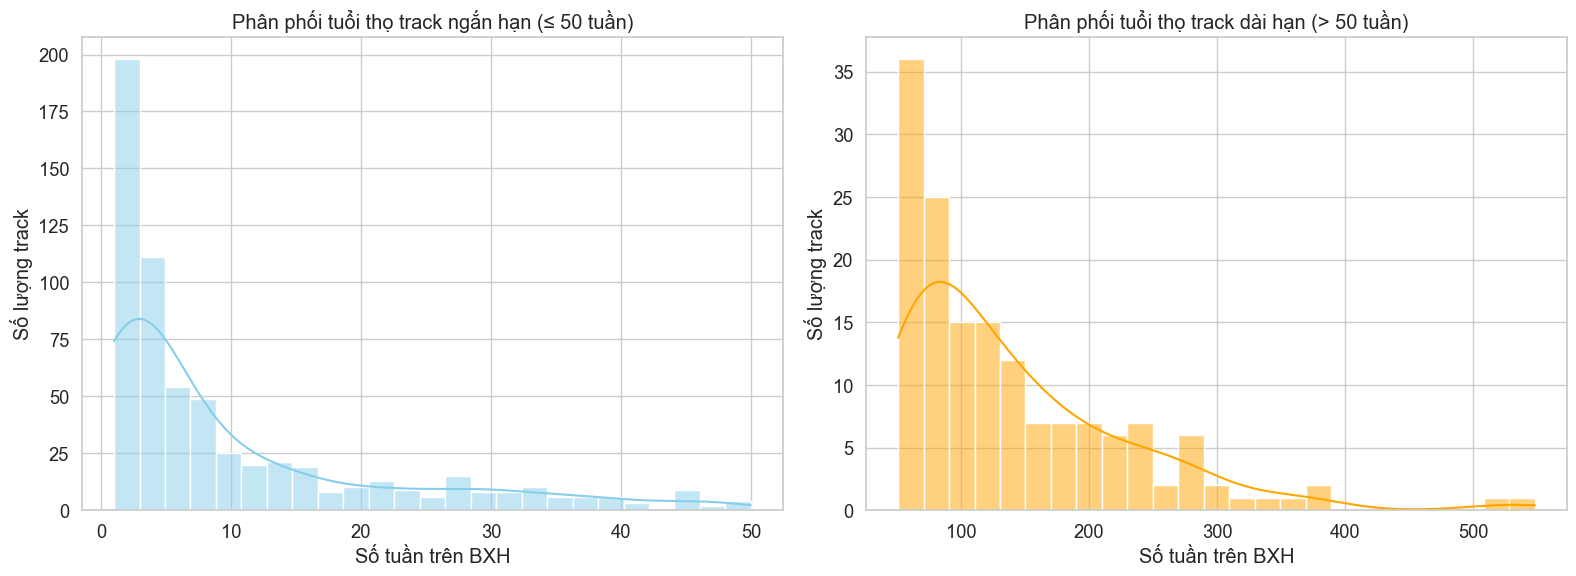
\includegraphics[width=\linewidth]{../graphics/data_top50/figure/11/EDA_world.png}
            \\[4pt] {\small \textbf{World}}
        \end{minipage}

        \caption{1.2 Tuổi thọ các bài hát trên BXH}
        \label{fig:energy-regions}
    \end{figure}


          \begin{itemize}
              \item \textbf{Kết luận: }
              \item Phần lớn bài hát có tuổi thọ ngắn, đa số bài hát chỉ trụ được dưới 10 tuần trên BXH => đặc trưng chung của BXH Top 50: hit bùng nổ nhanh nhưng cũng dễ rơi khỏi bảng.
              \item Vẫn tồn tại nhóm nhỏ có tuổi thọ dài (> 50 tuần), kéo dài đến 300–500 tuần.Những bài này thường là siêu hit toàn cầu hoặc gắn liền với văn hóa. 
              \item So sánh giữa các nước và thế giới: Ở cấp quốc gia, tuổi thọ thường ngắn hơn => thị trường có tính “nóng hổi”.Ở cấp thế giới, xuất hiện nhiều bài hát có tuổi thọ cực dài => tính bền vững và lan tỏa rộng.
              
          \end{itemize}

    \item\textbf{1.3 Độ biến động (volatility) trên BXH}


    \begin{figure}[H]
        \centering
        % Dòng 1
        \begin{minipage}{0.45\textwidth}
            \centering
            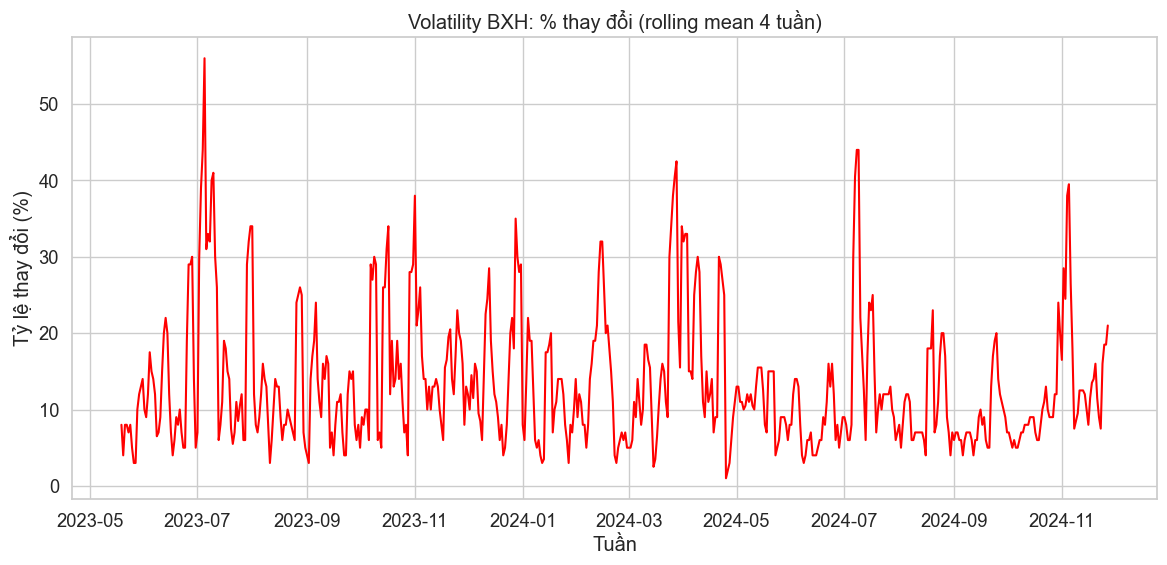
\includegraphics[width=\linewidth]{../graphics/data_top50/figure/12/EDA_usa.png}
            \\[4pt] {\small \textbf{USA}}
        \end{minipage}
        \hfill
        \begin{minipage}{0.45\textwidth}
            \centering
            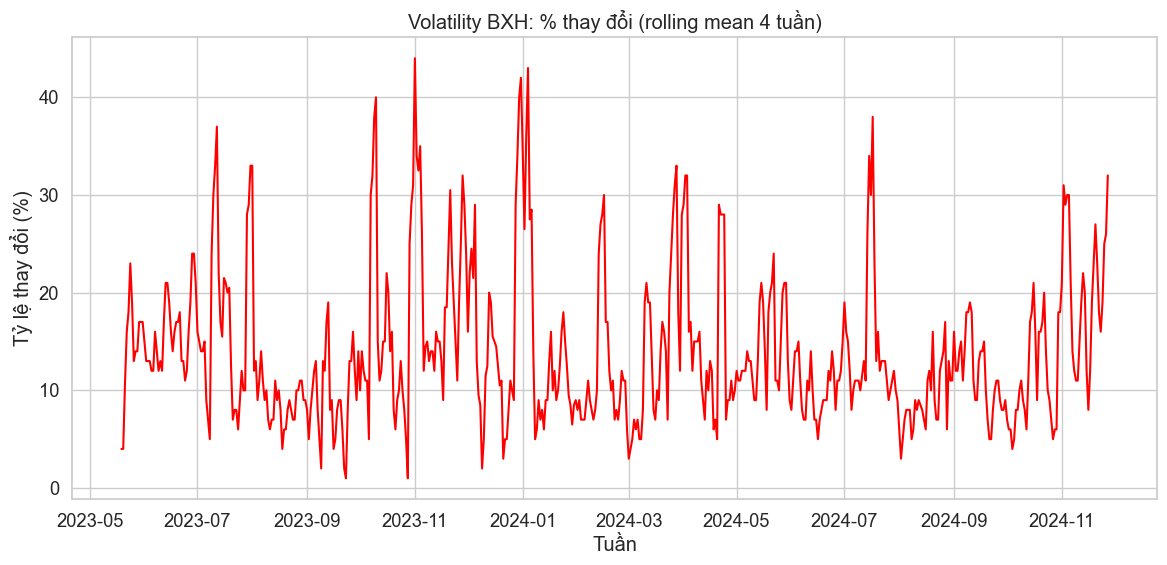
\includegraphics[width=\linewidth]{../graphics/data_top50/figure/12/EDA_uk.png}
            \\[4pt] {\small \textbf{UK}}
        \end{minipage}

        \vspace{0.4cm}

        % Dòng 2
        \begin{minipage}{0.45\textwidth}
            \centering
            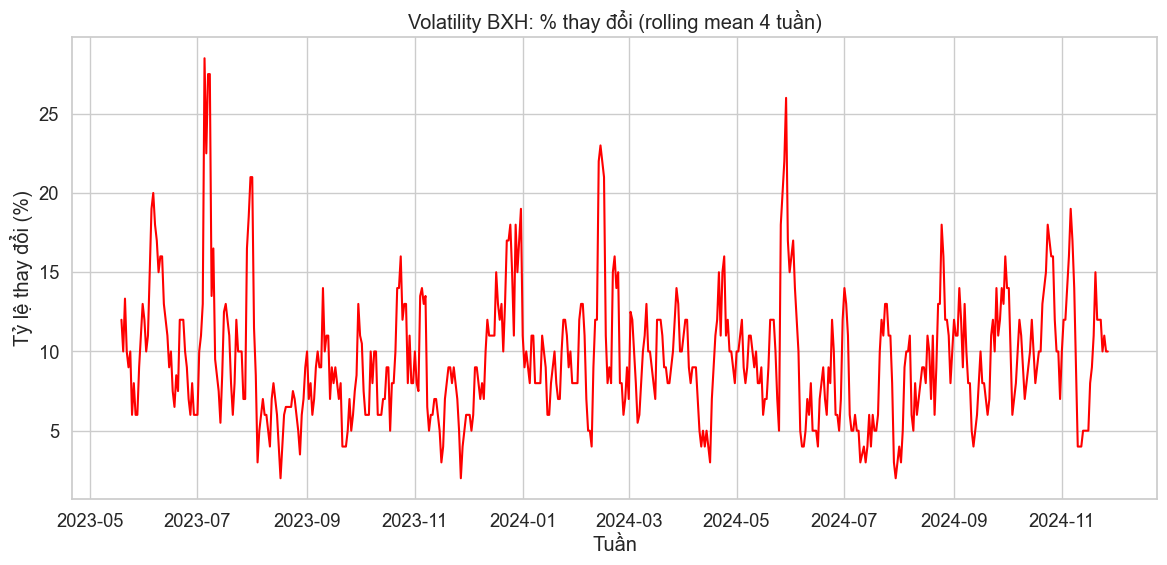
\includegraphics[width=\linewidth]{../graphics/data_top50/figure/12/EDA_south_korea.png}
            \\[4pt] {\small \textbf{Korea}}
        \end{minipage}
        \hfill
        \begin{minipage}{0.45\textwidth}
            \centering
            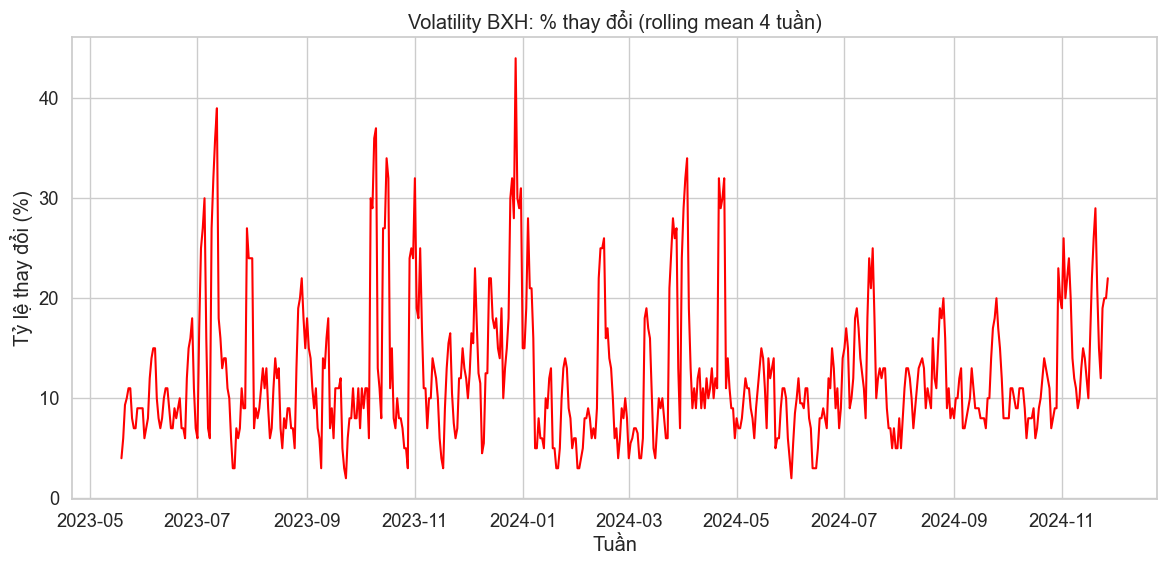
\includegraphics[width=\linewidth]{../graphics/data_top50/figure/12/EDA_world.png}
            \\[4pt] {\small \textbf{World}}
        \end{minipage}



        % Dòng 3
        \begin{minipage}{0.45\textwidth}
            \centering
            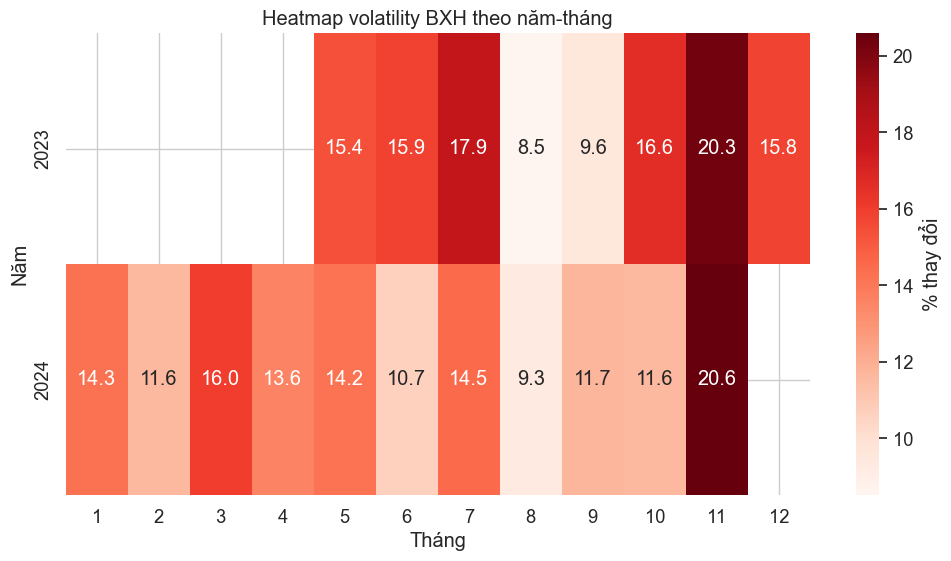
\includegraphics[width=\linewidth]{../graphics/data_top50/figure/14/EDA_uk.png}
            \\[4pt] {\small \textbf{UK}}
        \end{minipage}
        \hfill
        \begin{minipage}{0.45\textwidth}
            \centering
            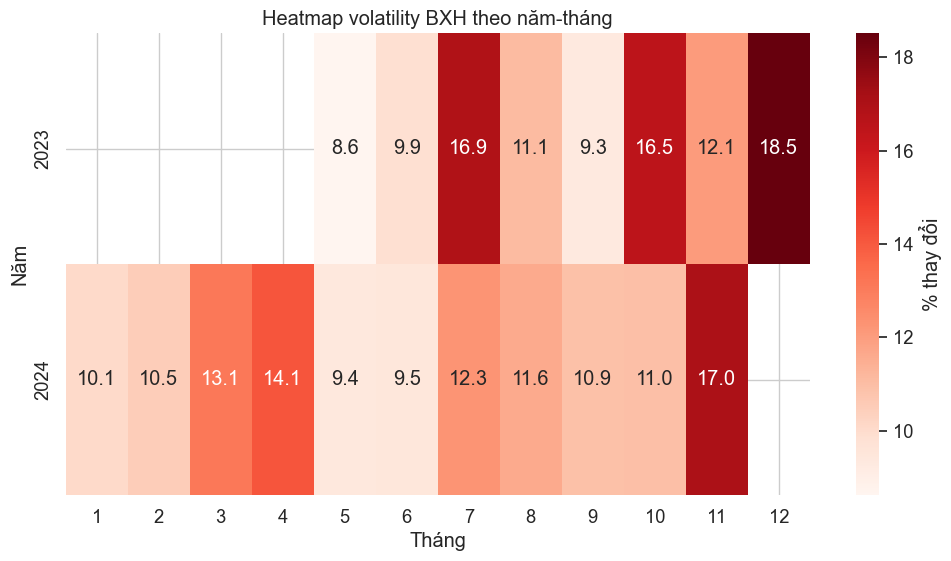
\includegraphics[width=\linewidth]{../graphics/data_top50/figure/14/EDA_world.png}
            \\[4pt] {\small \textbf{World}}
        \end{minipage}

        \caption{1.2 Độ biến động tổng quan trên BXH}
        \label{fig:energy-regions}

        
    \end{figure}



        \begin{itemize}
            \item \textbf{Kết luận: }
            \item Mức biến động cao ở nhiều thị trường lớn, Mỹ, Anh thường có volatility > 20–30\%\ trong nhiều giai đoạn. Cho thấy cạnh tranh gay gắt, các ca khúc nhanh chóng leo hạng và rời BXH
            \item Một số thị trường ổn định hơn Nhật, Ý, Tây Ban Nha có volatility thấp hơn (chủ yếu < 15\%\ ). Điều này phản ánh thị hiếu nghe nhạc ổn định, ít thay đổi đột ngột theo xu hướng.
            \item Đặc thù mùa vụ và sự kiện âm nhạc:
             Các đỉnh biến động thường rơi vào dịp cuối năm, mùa lễ hội.
               Ví dụ: giai đoạn cuối 2023 và giữa 2024 có nhiều peak volatility (đỉnh) đồng loạt ở nhiều nước.
        \end{itemize}

    

          
\end{itemize}


\textbf{2. Nghệ sĩ và Bài hát}

\begin{itemize}

    \item \textbf{2.1 Top 10 nghệ sĩ phổ biến}



    \begin{figure}[H]
        \centering
        % Dòng 1
        \begin{minipage}{0.45\textwidth}
            \centering
            \includegraphics[width=\linewidth]{../graphics/data_top50/figure/0/EDA_USA.png}
            \\[4pt] {\small \textbf{USA}}
        \end{minipage}
        \hfill
        \begin{minipage}{0.45\textwidth}
            \centering
            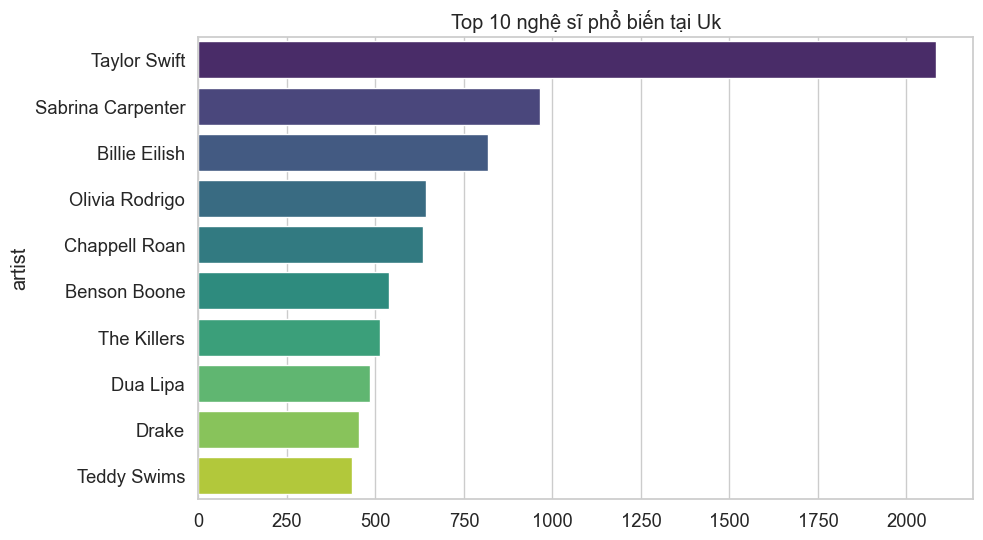
\includegraphics[width=\linewidth]{../graphics/data_top50/figure/0/EDA_uk.png}
            \\[4pt] {\small \textbf{UK}}
        \end{minipage}

        \vspace{0.4cm}

        % Dòng 2
        \begin{minipage}{0.45\textwidth}
            \centering
            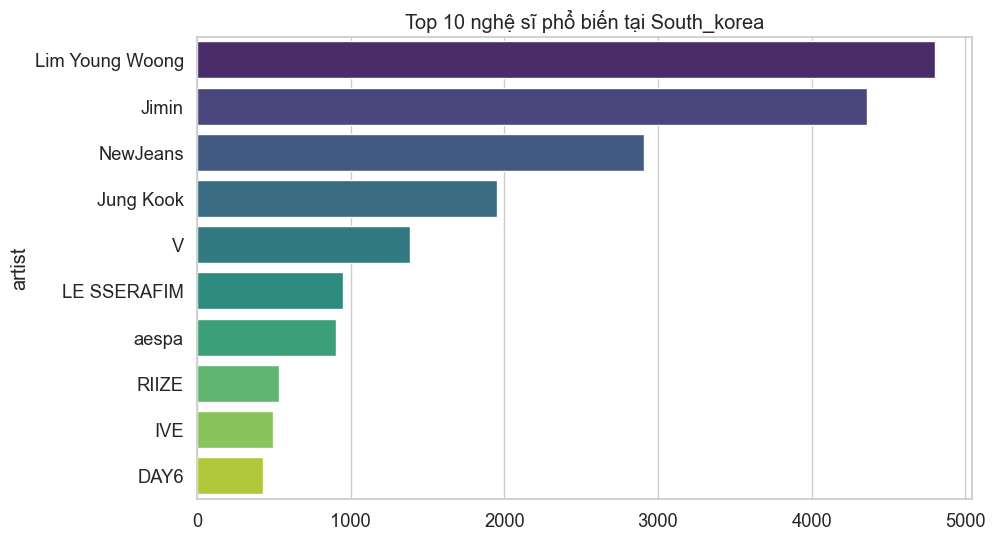
\includegraphics[width=\linewidth]{../graphics/data_top50/figure/0/EDA_south_korea.png}
            \\[4pt] {\small \textbf{Korea}}
        \end{minipage}
        \hfill
        \begin{minipage}{0.45\textwidth}
            \centering
            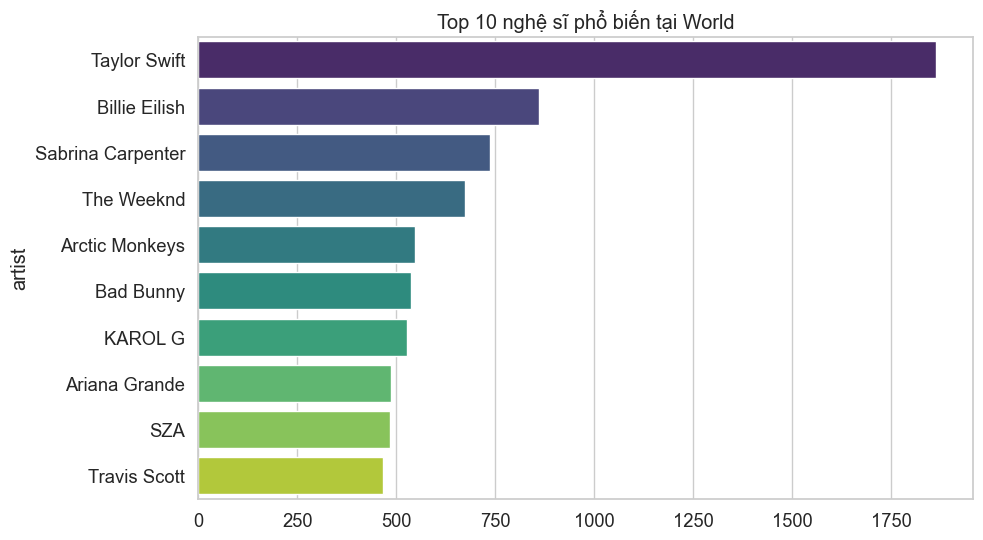
\includegraphics[width=\linewidth]{../graphics/data_top50/figure/0/EDA_world.png}
            \\[4pt] {\small \textbf{World}}
        \end{minipage}



        
        \caption{Top 10 nghệ sĩ nổi bật nhất}
        \label{fig:energy-regions}
    \end{figure}
    
        \begin{itemize}
            \item \textbf{Kết luận: }
            \item Nhìn chung đa số quốc gia có nghệ sĩ nội địa thống trị: ví dụ Emilia, Luck Ra (Argentina), Werenoi (France), Geolier, Tedua (Italy), Mrs. GREEN APPLE, YOASOBI (Japan), Peso Pluma (Mexico), Lim Young Woong, BTS members, NewJeans (Korea).
            \item Riêng thị trường Âu–Mỹ vẫn nổi bật với những ngôi sao toàn cầu: Taylor Swift, Billie Eilish, Drake, Bad Bunny, KAROL G… thường xuyên góp mặt cả ở BXH quốc gia và World.
            \item Có sự khác biệt rõ rệt giữa thị hiếu nội địa và toàn cầu: Nhật, Hàn Quốc chủ yếu nghệ sĩ bản địa; trong khi BXH World và Mỹ/UK có nhiều nghệ sĩ đa quốc gia.
        \end{itemize}







    \item \textbf{2.2 Bài hát theo độ hot}



    \begin{figure}[H]
        \centering
        % Dòng 1
        \begin{minipage}{0.4\textwidth}
            \centering
            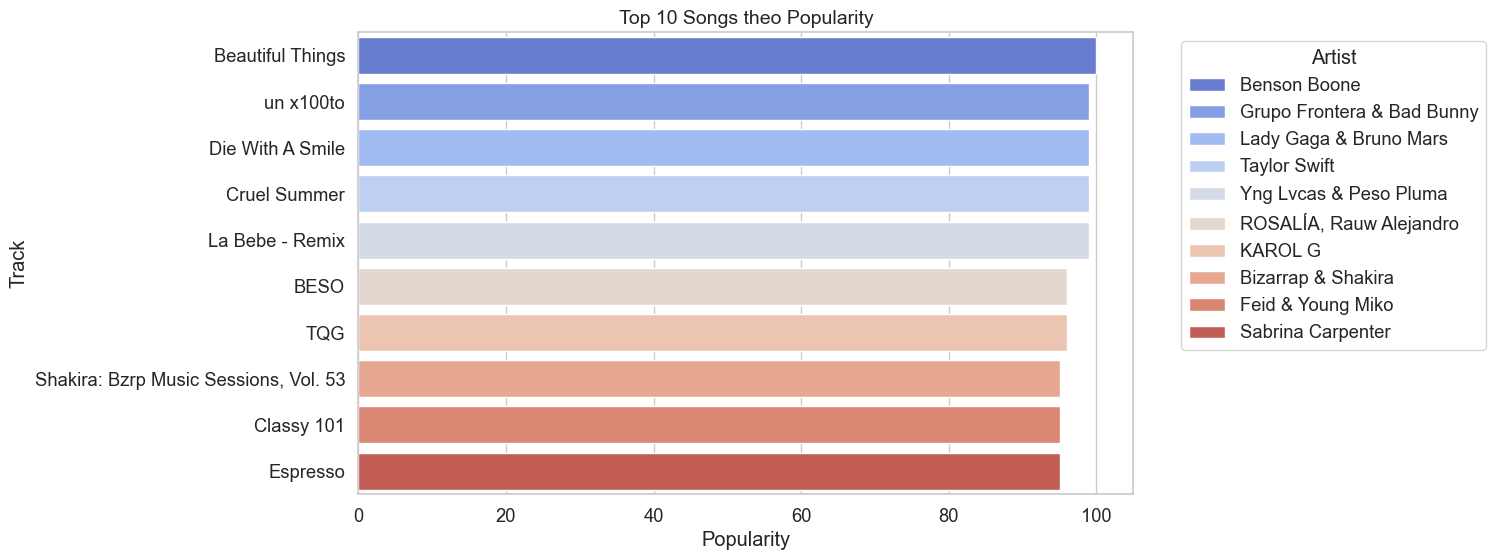
\includegraphics[width=\linewidth]{../graphics/data_top50/figure/2/EDA_argentina.png}
            \\[4pt] {\small \textbf{Argentina}}
        \end{minipage}
        \hfill
        \begin{minipage}{0.4\textwidth}
            \centering
            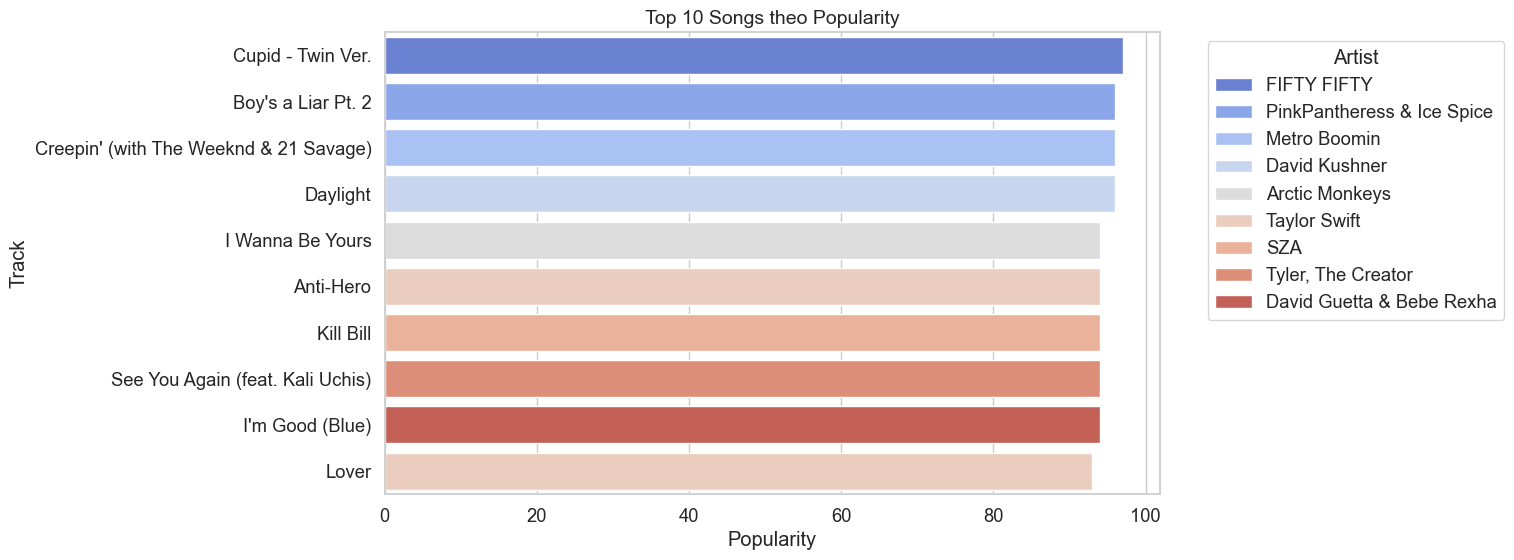
\includegraphics[width=\linewidth]{../graphics/data_top50/figure/2/EDA_uk.png}
            \\[4pt] {\small \textbf{UK}}
        \end{minipage}

        \vspace{0.4cm}

        % Dòng 2
        \begin{minipage}{0.4\textwidth}
            \centering
            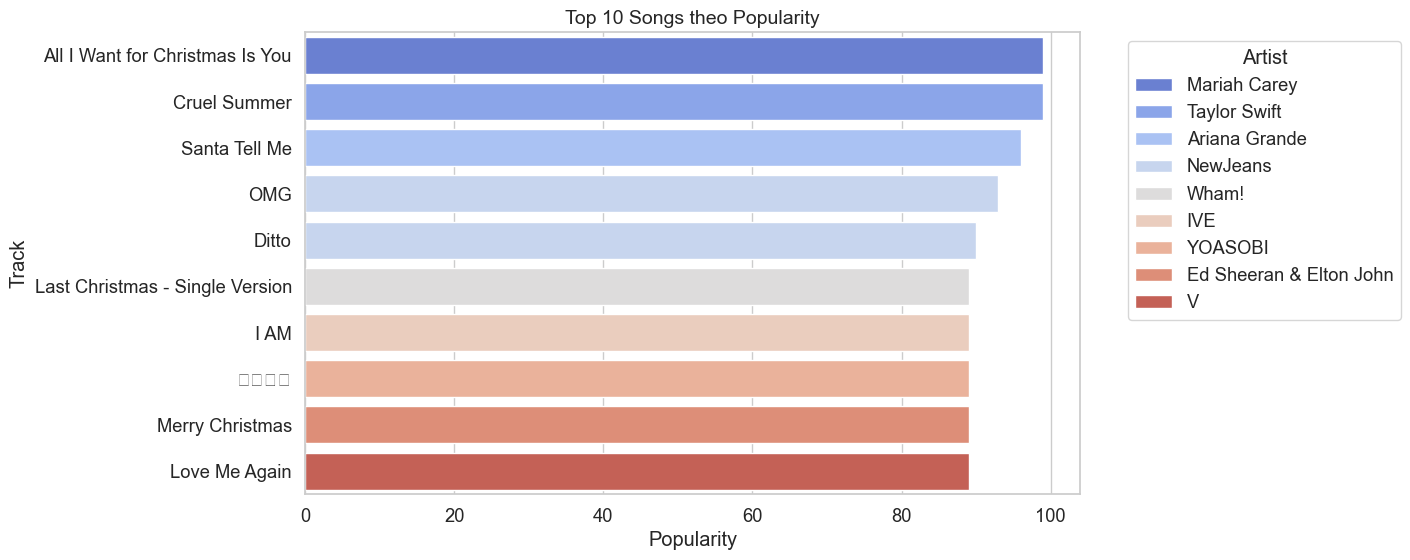
\includegraphics[width=\linewidth]{../graphics/data_top50/figure/2/EDA_japan.png}
            \\[4pt] {\small \textbf{Japan}}
        \end{minipage}
        \hfill
        \begin{minipage}{0.4\textwidth}
            \centering
            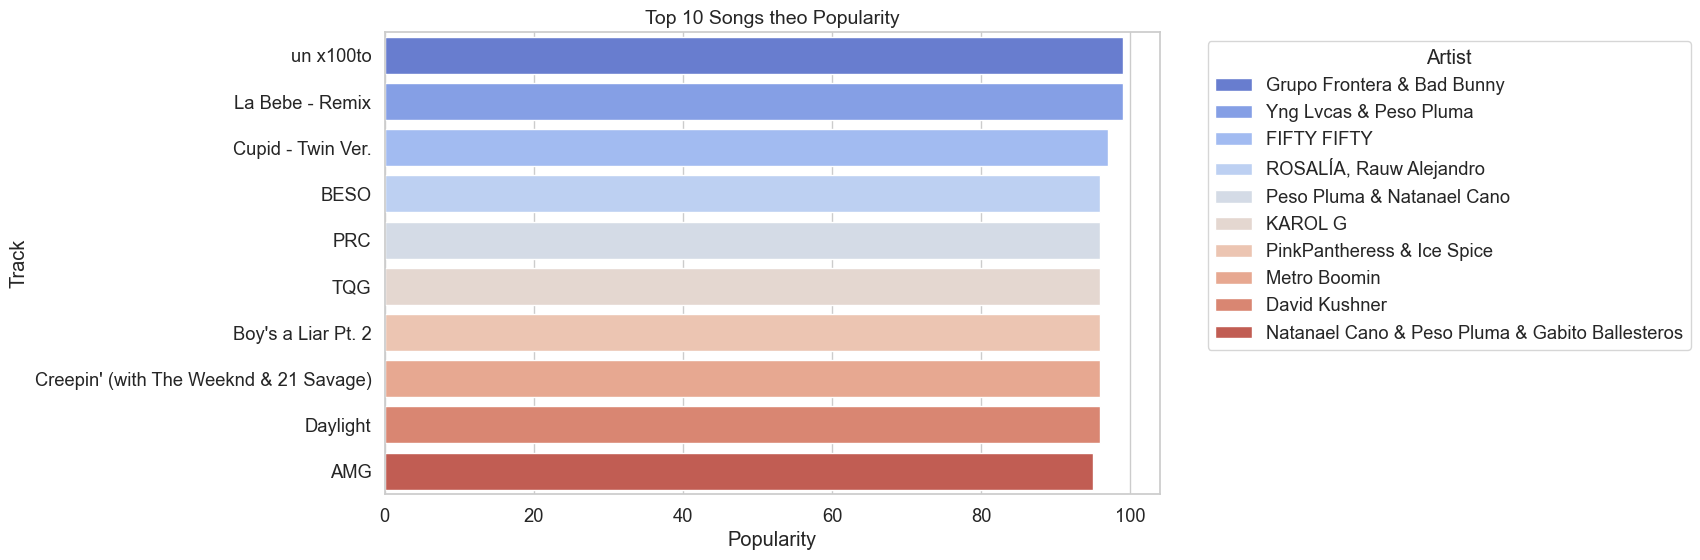
\includegraphics[width=\linewidth]{../graphics/data_top50/figure/2/EDA_world.png}
            \\[4pt] {\small \textbf{World}}
        \end{minipage}
        
        \caption{Top 10 bài hát trụ nổi nhất}
        \label{fig:energy-regions}

        \vspace{0.4cm}
        \begin{minipage}{1\textwidth}
            \centering
            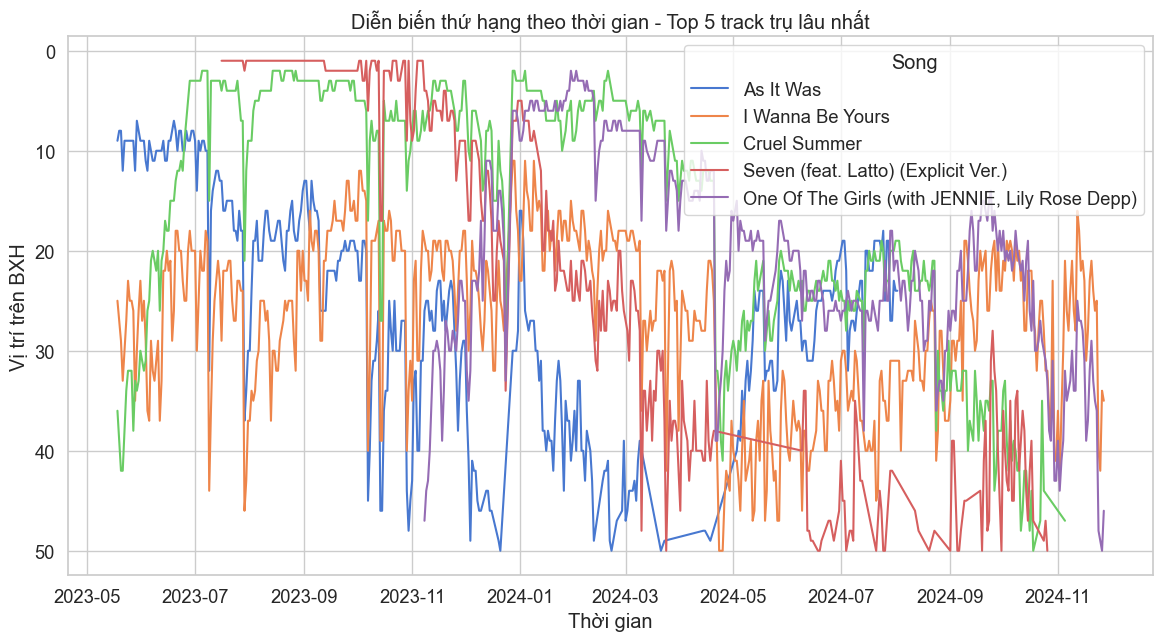
\includegraphics[width=\linewidth]{../graphics/data_top50/figure/17/EDA_world.png}
            \\[4pt] {\small \textbf{World}}
        \end{minipage}
        
        \caption{Top 5 bài hát trụ lâu nhất}
         \label{fig:energy-regions}

     \end{figure}

                % Dòng 2
        


      
    
   

         \begin{itemize}
             \item \textbf{Kết luận: }
             \item Top 10 bài hát phổ biến: mỗi quốc gia có “quốc ca nội địa” riêng , trong khi BXH World lại nổi bật với các siêu hit toàn cầu .
             
             \item  Top 5 bài hát trụ lâu nhất : Cho thấy sự khác biệt giữa các thị trường: US/UK có những bản hit lâu bền, Hàn Quốc ghi dấu với loạt K-pop nổi bật, còn các nước Mỹ Latin có nhiều ca khúc trụ lâu thuộc dòng nhạc địa phương. Trên BXH World, một số siêu hit quốc tế  thể hiện sức hút bền vững, duy trì thứ hạng cao trong nhiều tháng.

             
             \item So sánh quốc gia – thế giới cho thấy: bài hát nội địa thường nổi trong nước nhưng ít khi bền vững toàn cầu, ngược lại siêu hit quốc tế có sức lan tỏa rộng và trụ lâu hơn

             
         \end{itemize}
\end{itemize}




\textbf{3. Thể loại}
\begin{itemize}
    \item \textbf{3.1 Top 10 thể loại phổ biến}


    \begin{figure}[H]
        \centering
        % Dòng 1
        \begin{minipage}{0.35\textwidth}
            \centering
            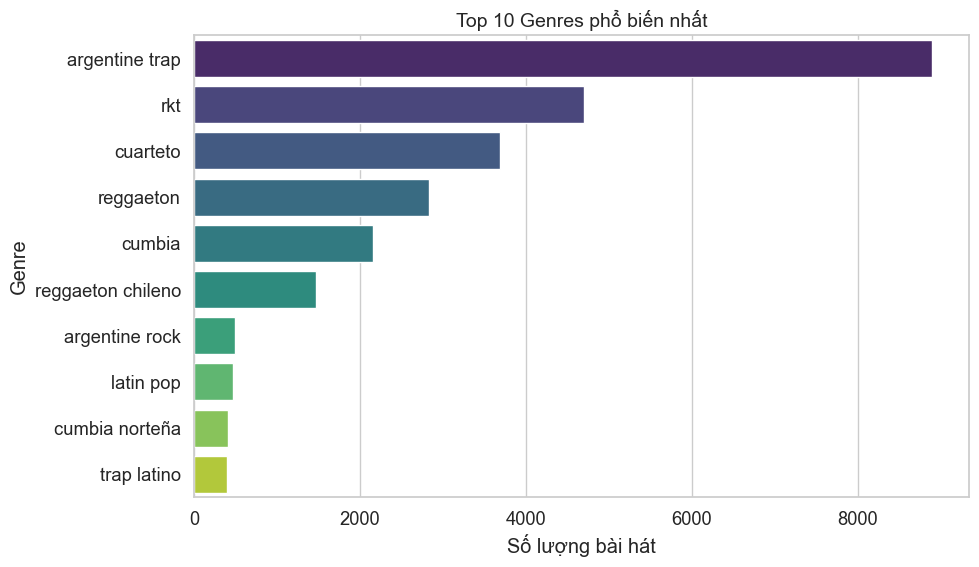
\includegraphics[width=\linewidth]{../graphics/data_top50/figure/1/EDA_argentina.png}
            \\[4pt] {\small \textbf{Argentina}}
        \end{minipage}
        \hfill
        \begin{minipage}{0.35\textwidth}
            \centering
            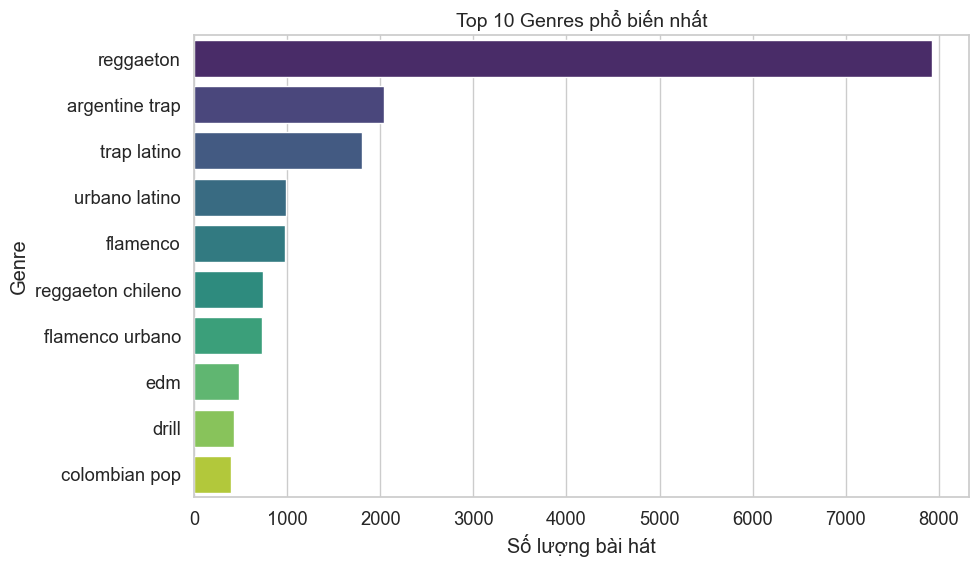
\includegraphics[width=\linewidth]{../graphics/data_top50/figure/1/EDA_spain.png}
            \\[4pt] {\small \textbf{Spain}}
        \end{minipage}

        \vspace{0.4cm}

        % Dòng 2
        \begin{minipage}{0.35\textwidth}
            \centering
            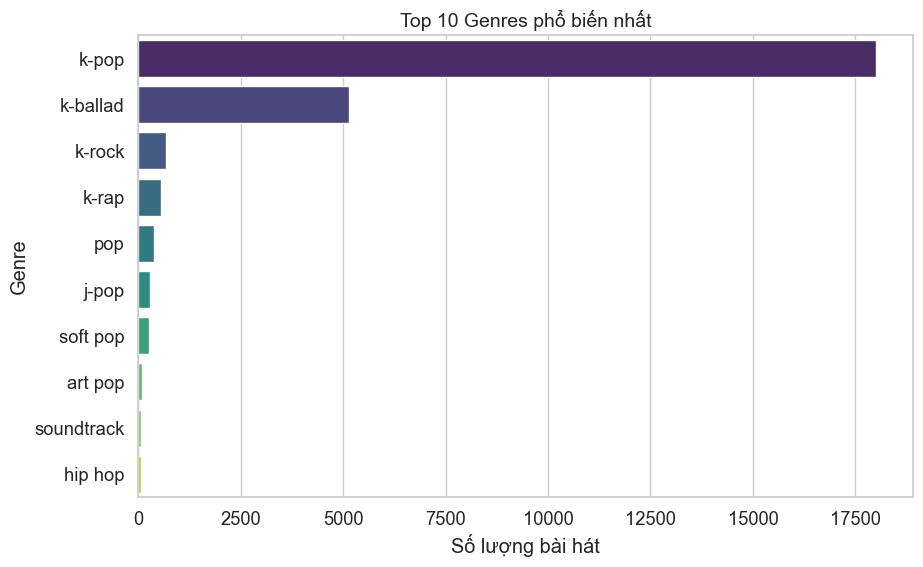
\includegraphics[width=\linewidth]{../graphics/data_top50/figure/1/EDA_south_korea.png}
            \\[4pt] {\small \textbf{Korea}}
        \end{minipage}
        \hfill
        \begin{minipage}{0.35\textwidth}
            \centering
            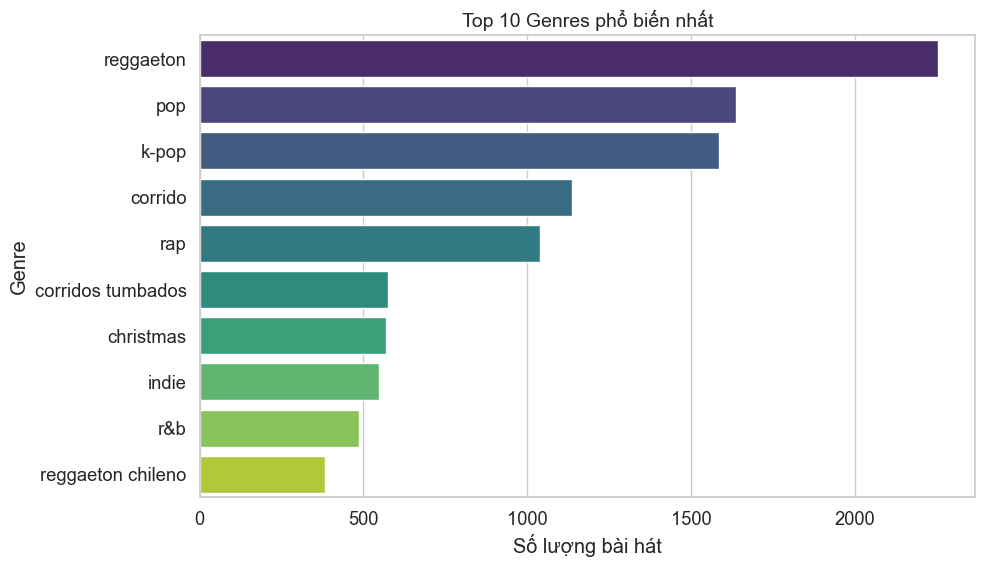
\includegraphics[width=\linewidth]{../graphics/data_top50/figure/1/EDA_world.png}
            \\[4pt] {\small \textbf{World}}
        \end{minipage}



        
        \caption{Top 10 thể loại nổi bật nhất}
        \label{fig:energy-regions}
    \end{figure}
    

    
    \begin{itemize}
        \item \textbf{Kết luận: }
        \item Mỗi quốc gia có thể loại bản địa thống trị, ví dụ:Argentina (Argentine trap, RKT, cuarteto), Japan (J-pop, Anime, J-rock), ..
        
        % \begin{itemize}
        %     \item Argentina => Argentine trap, RKT, cuarteto

        %      \item France => French rap, French R \&\ B

        %         \item Italy => Italian trap, Canzone napoletana

        %         \item Japan => J-pop, Anime, J-rock

        %        \item Mexico => Corrido, Corridos tumbados, Banda

        %       \item Korea => K-pop, K-ballad

        %    \item Spain => Reggaeton, Flamenco

        %      \item US/UK => Pop, Rap, Country, Alternative rock.
        % \end{itemize}

        \item Sự khác biệt văn hoá rõ rệt: Nhật – Hàn nghiêng về nhạc bản địa (J-pop, K-pop), Mexico – LATAM mạnh về reggaeton/corrido, còn Âu–Mỹ giữ vị thế với pop/rap.
        \item Xu hướng toàn cầu: Một số thể loại vượt biên giới mạnh mẽ (reggaeton, trap, pop, rap) => lan toả sang nhiều thị trường khác nhau.
    \end{itemize}

   \item \textbf{3.1 Xu hướng thể loại theo thời gian}


   
    \begin{figure}[H]
        \centering
        % Dòng 1
        \begin{minipage}{0.45\textwidth}
            \centering
            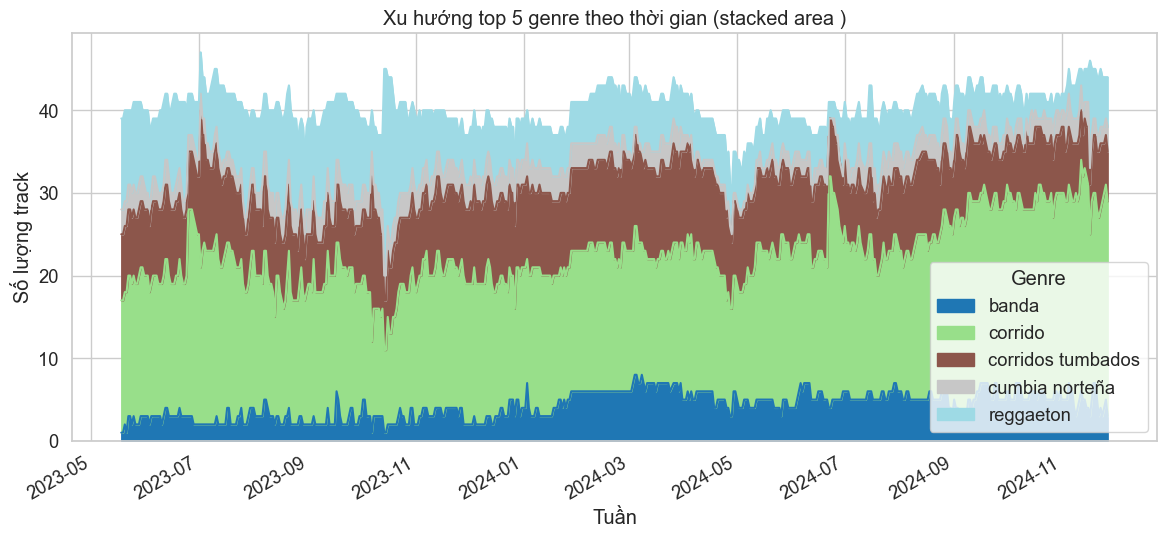
\includegraphics[width=\linewidth]{../graphics/data_top50/figure/25/EDA_mexico.png}
            \\[4pt] {\small \textbf{Mexico}}
        \end{minipage}
        \hfill
        \begin{minipage}{0.45\textwidth}
            \centering
            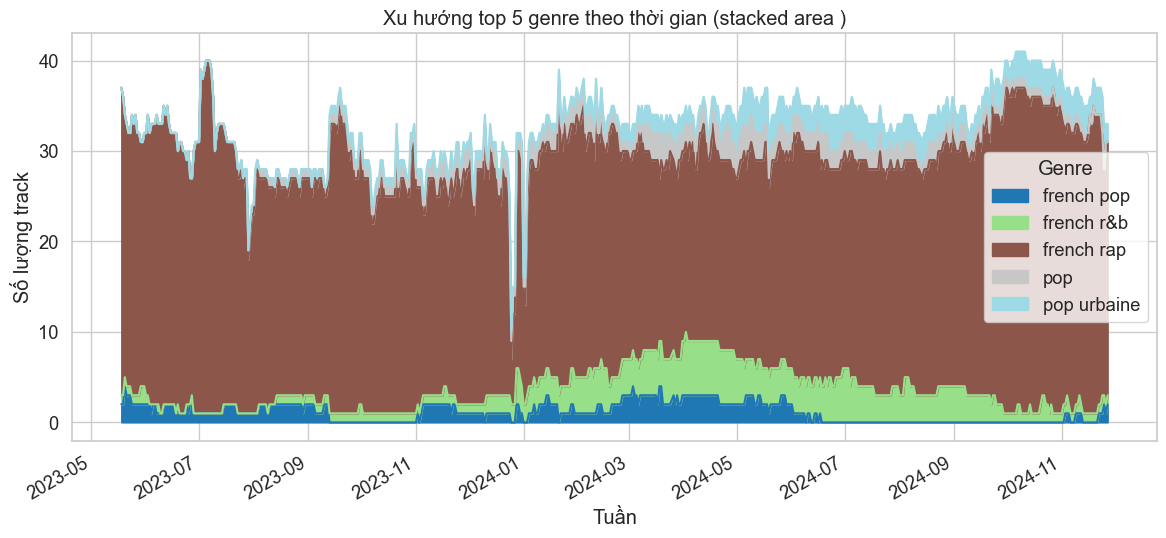
\includegraphics[width=\linewidth]{../graphics/data_top50/figure/25/EDA_france.png}
            \\[4pt] {\small \textbf{France}}
        \end{minipage}

        \vspace{0.4cm}

        % Dòng 2
        \begin{minipage}{0.45\textwidth}
            \centering
            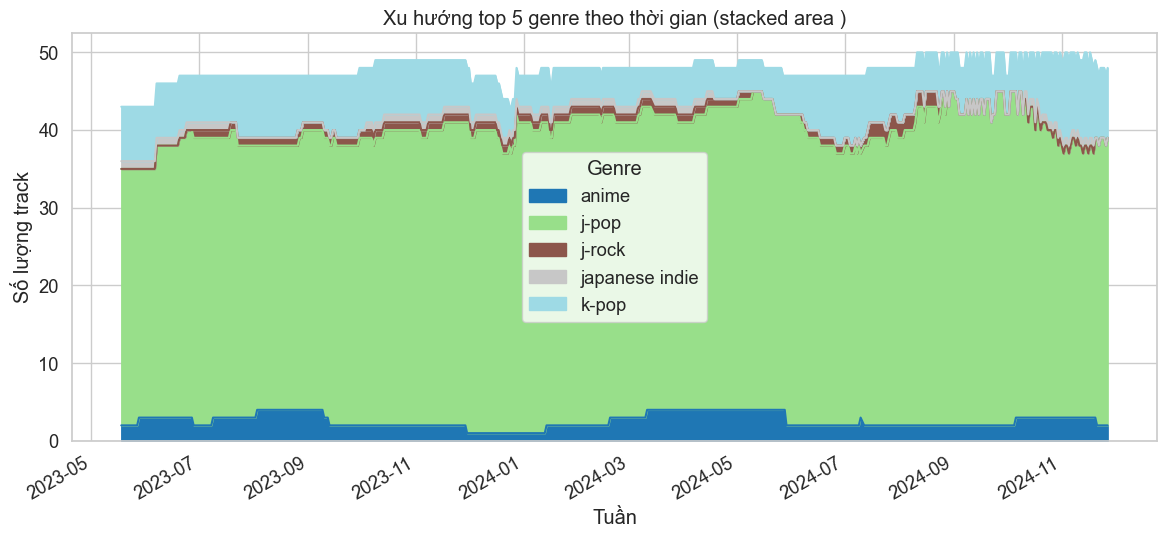
\includegraphics[width=\linewidth]{../graphics/data_top50/figure/25/EDA_japan.png}
            \\[4pt] {\small \textbf{Japan}}
        \end{minipage}
        \hfill
        \begin{minipage}{0.45\textwidth}
            \centering
            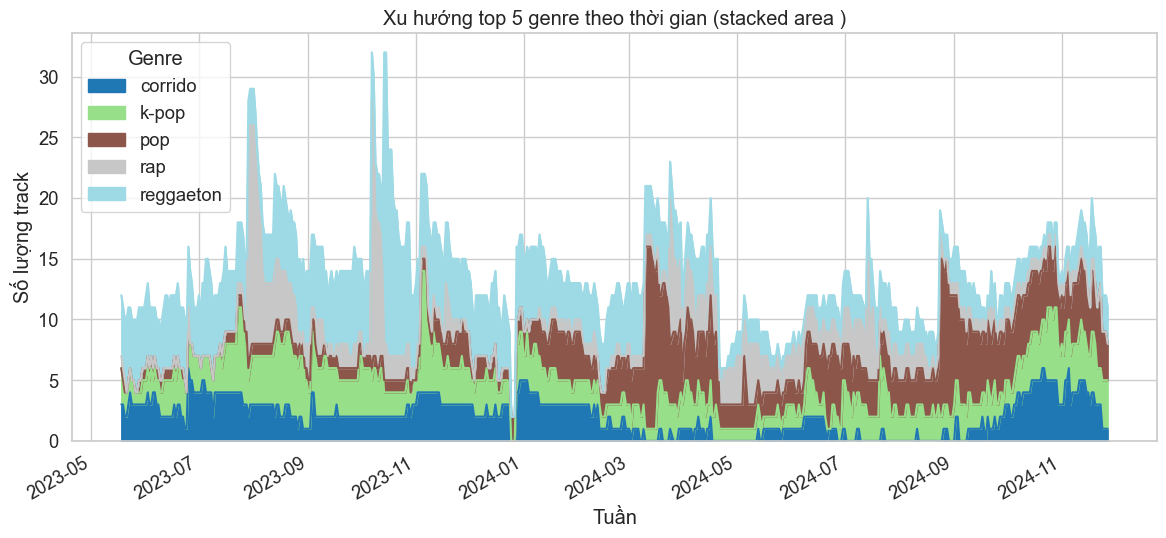
\includegraphics[width=\linewidth]{../graphics/data_top50/figure/25/EDA_world.png}
            \\[4pt] {\small \textbf{World}}
        \end{minipage}

        \caption{Top 10 thể loại nổi bật nhất}
    \end{figure}

    \begin{itemize}
        \item \textbf{Kết luận:}
        \item Genre bản địa áp đảo ổn định: J-pop (Japan), K-pop/K-ballad (Korea), French rap (France), Italian trap (Italy).
        \item Đa dạng nhất: Mexico – sự kết hợp của corrido, banda, tumbados, reggaeton, cumbia norteña.

        \item Khép kín: Nhật và Hàn hầu như chỉ nghe nhạc nội địa.
        \item Thể loại Latin (reggaeton, corrido, trap latino) tăng mạnh tại Argentina, Mexico, Spain và có sức lan tỏa sang thị trường quốc tế.
        \item Thể loại mùa vụ như Christmas nổi bật ở US/UK, tạo các đỉnh ngắn hạn cuối năm.

        \item Thị trường toàn cầu (World) cho thấy sự kết hợp của reggaeton, K-pop và pop/rap, phản ánh sự giao thoa văn hoá âm nhạc xuyên biên giới.
    \end{itemize}

    \begin{figure}[H]
        \centering
        % Dòng 1
        \begin{minipage}{0.45\textwidth}
            \centering
            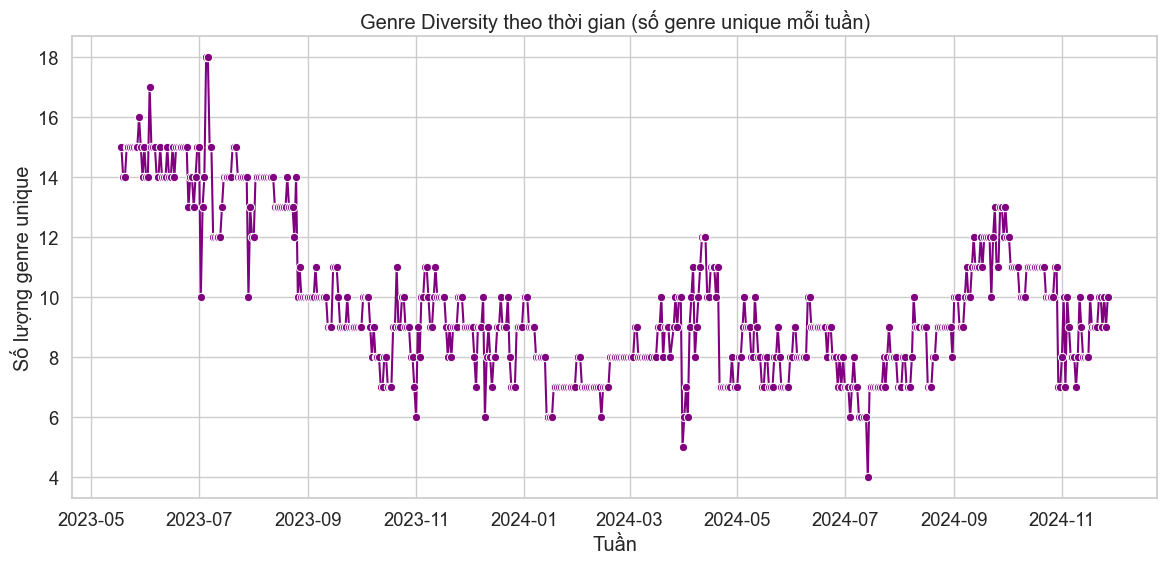
\includegraphics[width=\linewidth]{../graphics/data_top50/figure/24/EDA_usa.png}
            \\[4pt] {\small \textbf{USA}}
        \end{minipage}
        \hfill
        \begin{minipage}{0.45\textwidth}
            \centering
            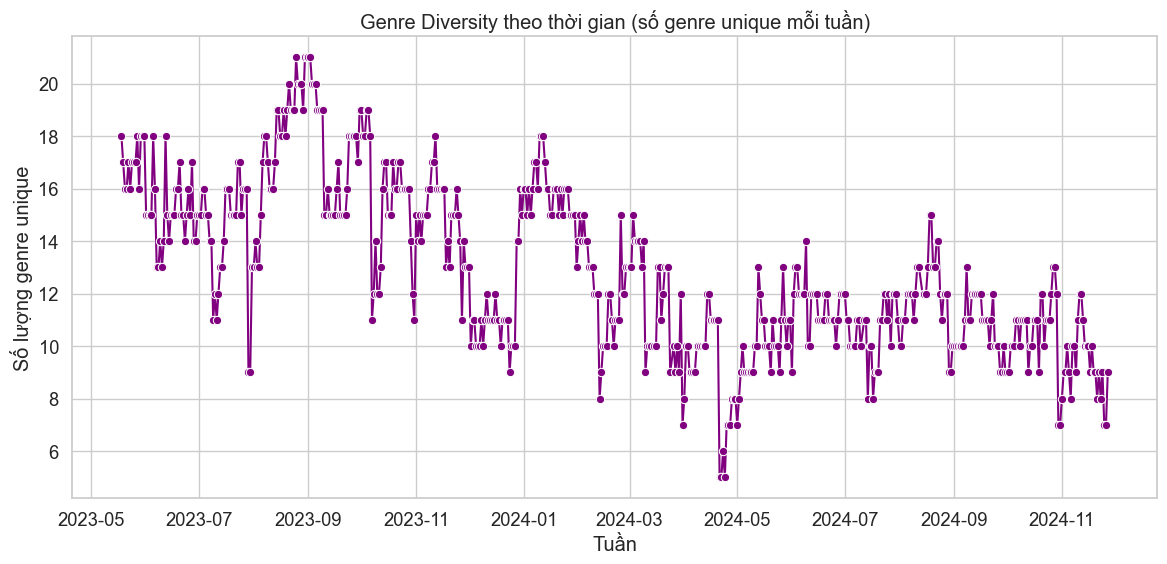
\includegraphics[width=\linewidth]{../graphics/data_top50/figure/24/EDA_uk.png}
            \\[4pt] {\small \textbf{UK}}
        \end{minipage}

        \vspace{0.4cm}

        % Dòng 2
        \begin{minipage}{0.45\textwidth}
            \centering
            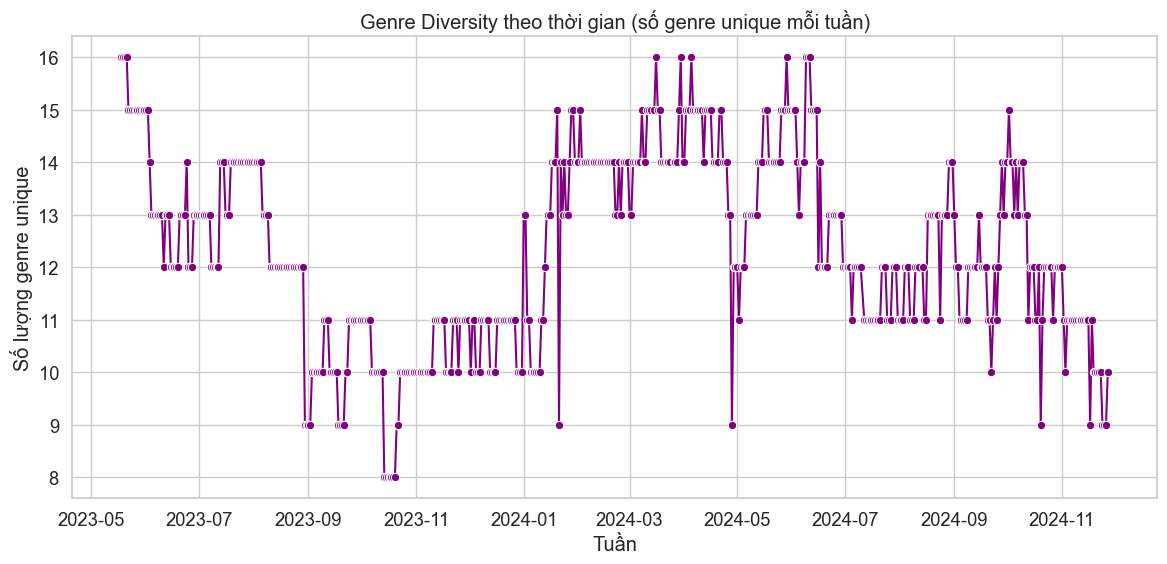
\includegraphics[width=\linewidth]{../graphics/data_top50/figure/24/EDA_spain.png}
            \\[4pt] {\small \textbf{Spain}}
        \end{minipage}
        \hfill
        \begin{minipage}{0.45\textwidth}
            \centering
            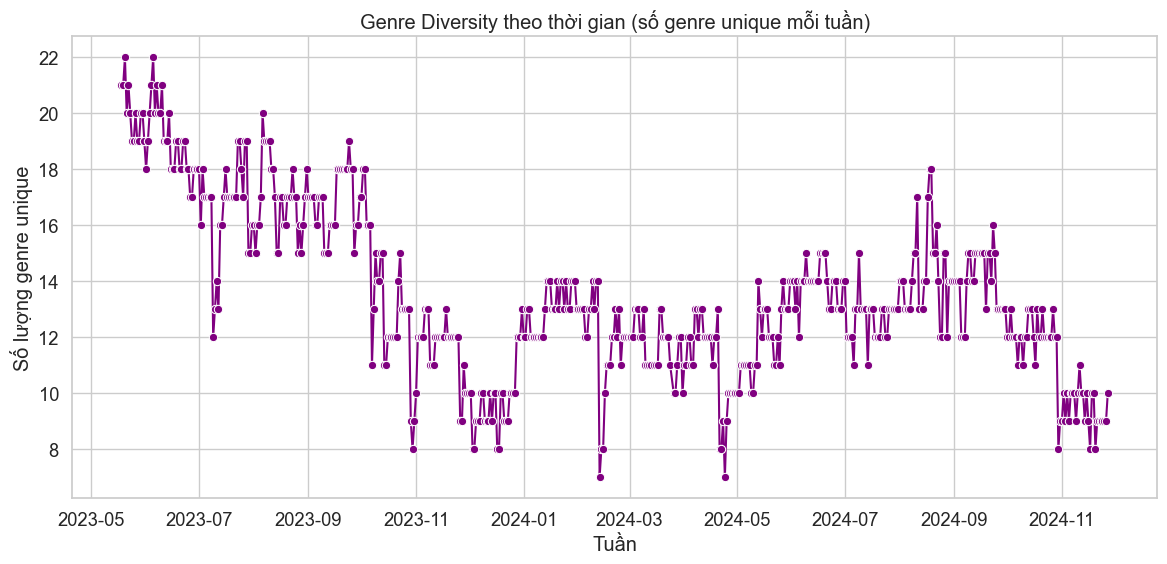
\includegraphics[width=\linewidth]{../graphics/data_top50/figure/24/EDA_world.png}
            \\[4pt] {\small \textbf{World}}
        \end{minipage}



        



        
        \caption{Độ đa dạng theo tuần}
    \end{figure}


    \begin{itemize}
        \item \textbf{Kết luận: }
        \item Khác biệt thị trường: US và World đa dạng nhất (10–22 genre/tuần), trong khi Nhật, Hàn, Ý khá tập trung (5–12 genre, chủ yếu J-pop, K-pop, Italian trap).

        \item Xu hướng mùa vụ: US/UK xuất hiện nhiều genre phụ cuối năm (Christmas, country, grime), còn Nhật/Hàn ổn định quanh 5–8 genre.

        \item Mỹ Latin (Argentina, Mexico, Spain): trung bình 8–15 genre, xoay quanh reggaeton, corrido, trap latino => ít bùng nổ thể loại mới.
        \item  Nhật Bản \&\ Hàn Quốc: số genre unique thấp và ổn định (5–8/tuần), gần như bị áp đảo bởi J-pop (Japan) và K-pop/K-ballad (Korea).
    \end{itemize}
\end{itemize}


 


\textbf{4. Đặc trưng âm nhạc}
\begin{itemize}
    \item \textbf{4.1 Đặc trưng energy}
    \begin{itemize}


   \begin{figure}[H]
        \centering
        % Dòng 1
        \begin{minipage}{0.45\textwidth}
            \centering
            \includegraphics[width=\linewidth]{../graphics/data_top50/figure/3/EDA_USA.png}
            \\[4pt] {\small \textbf{USA}}
        \end{minipage}
        \hfill
        \begin{minipage}{0.45\textwidth}
            \centering
            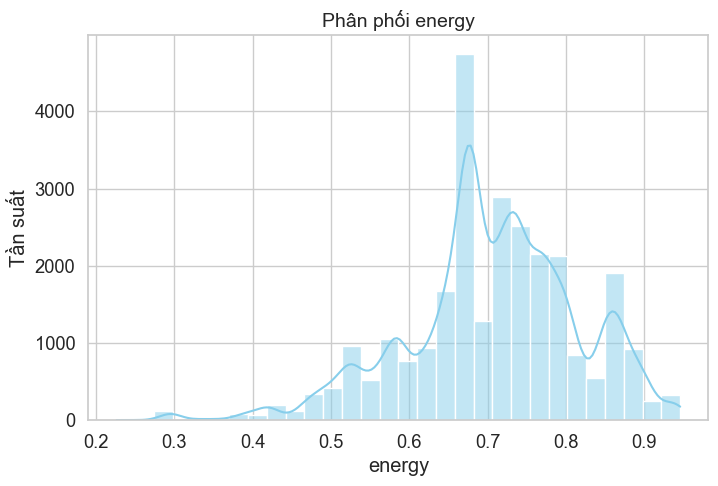
\includegraphics[width=\linewidth]{../graphics/data_top50/figure/3/EDA_spain.png}
            \\[4pt] {\small \textbf{Spain}}
        \end{minipage}

        \vspace{0.4cm}

        % Dòng 2
        \begin{minipage}{0.45\textwidth}
            \centering
            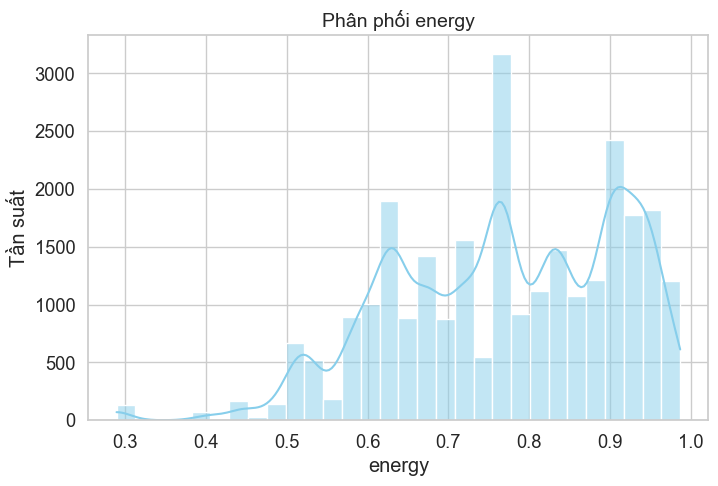
\includegraphics[width=\linewidth]{../graphics/data_top50/figure/3/EDA_japan.png}
            \\[4pt] {\small \textbf{Japan}}
        \end{minipage}
        \hfill
        \begin{minipage}{0.45\textwidth}
            \centering
            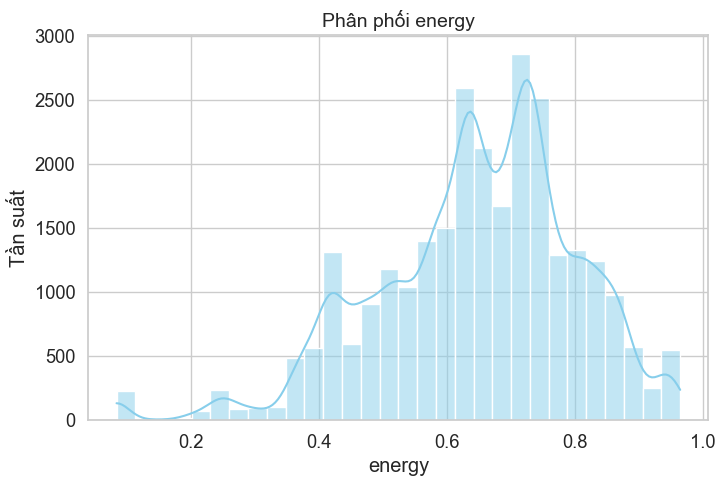
\includegraphics[width=\linewidth]{../graphics/data_top50/figure/3/EDA_world.png}
            \\[4pt] {\small \textbf{World}}
        \end{minipage}



        
        \caption{Đặc trưng energy}
        \label{fig:energy-regions}
    \end{figure}
    
        \item \textbf{Kết luận:}
        \item Tồn tại sự khác biệt rõ rệt về mức năng lượng ưa chuộng giữa các thị trường, phản ánh sự đa dạng trong văn hóa nghe nhạc và đặc tính thể loại bản địa.
        \item Phân cực rõ ràng giữa hai nhóm thị trường:
        \begin{itemize}
            \item Nhóm năng lượng cao \& đa dạng: Hầu hết các quốc gia như Argentina, France, UK, USA có phân phối energy. trải dài từ 0.2 đến 1.0 => thị hiếu âm nhạc tại đây rất đa dạng, chấp nhận cả những bài nhạc trầm lắng (energy thấp) lẫn những bài cực kỳ sôi động (energy cao).
            \item Nhóm năng lượng trung bình \& "ôn hòa": Italy và Spain có phân phối giới hạn trong khoảng 0.2 đến 0.9 => top âm nhạc tại đây có xu hướng thiếu vắng những bài hát có mức năng lượng cực cao, phù hợp với các thể loại mang tính chất nhẹ nhàng, êm dịu hơn như Pop, Ballad, hoặc Latin truyền thống.
        \end{itemize}
        \item Japan là trường hợp đặc biệt: Phân phối energy của Nhật bắt đầu từ 0.3 đến 1.0. Ngưỡng năng lượng tối thiểu cao hơn => ưa chuộng những bản nhạc có tiết tấu nhanh và sôi động ngay từ đầu, ít các bài hát có nhịp độ chậm và trầm buồn
        \item Thị trường toàn cầu (World) là sự kết hợp: Phân phối energy của World phủ rộng từ 0.2 đến 1.0, phản ánh chính xác việc nó là sự tổng hòa của tất cả các thị trường, thể hiện sự đa dạng và toàn diện nhất về mức năng lượng.
    \end{itemize}


    \item\textbf{4.2 Đặc trưng tempo}
 
           \begin{figure}[H]
        \centering
        % Dòng 1
        \begin{minipage}{0.45\textwidth}
            \centering
            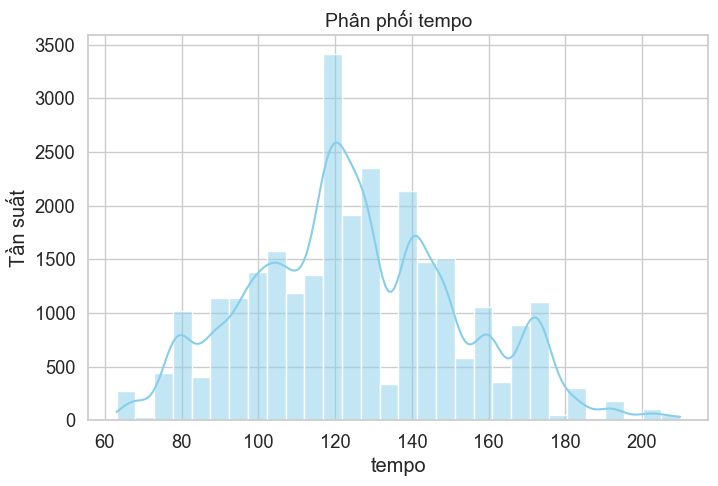
\includegraphics[width=\linewidth]{../graphics/data_top50/figure/4/EDA_uk.png}
            \\[4pt] {\small \textbf{UK}}
        \end{minipage}
        \hfill
        \begin{minipage}{0.45\textwidth}
            \centering
            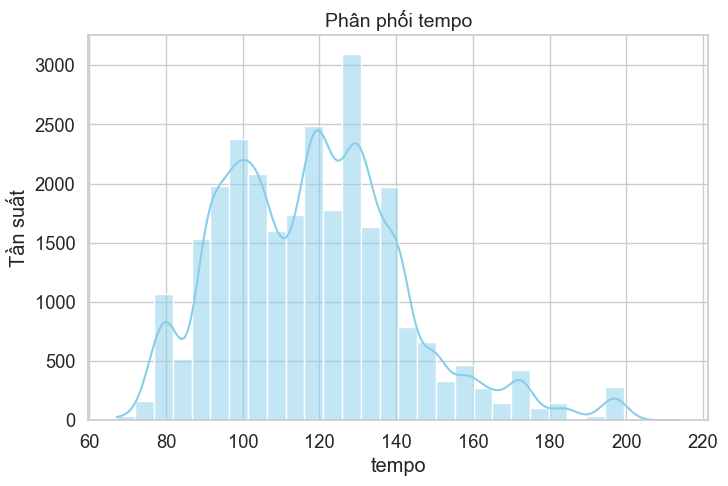
\includegraphics[width=\linewidth]{../graphics/data_top50/figure/4/EDA_italy.png}
            \\[4pt] {\small \textbf{italy}}
        \end{minipage}

        \vspace{0.4cm}

        % Dòng 2
        \begin{minipage}{0.45\textwidth}
            \centering
            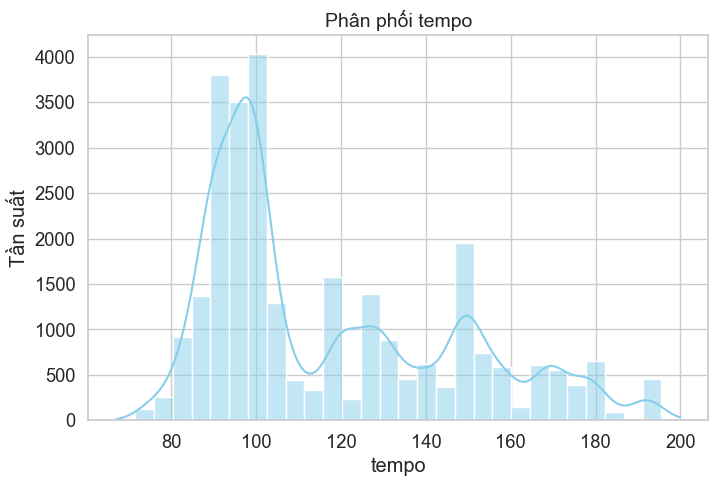
\includegraphics[width=\linewidth]{../graphics/data_top50/figure/4/EDA_argentina.png}
            \\[4pt] {\small \textbf{Argentian}}
        \end{minipage}
        \hfill
        \begin{minipage}{0.45\textwidth}
            \centering
            \includegraphics[width=\linewidth]{../graphics/data_top50/figure/4/EDA_world.png}
            \\[4pt] {\small \textbf{World}}
        \end{minipage}



        
        \caption{Đặc trưng tempo}
        \label{fig:energy-regions}
    \end{figure}
    

    
            \begin{itemize}
        \item \textbf{Kết luận: }

        \item Tồn tại sự tương đồng lớn về phân phối nhịp độ giữa các thị trường chủ chốt. Các nước như Argentina, Mexico, Nhật Bản (Japan) và Hàn Quốc (South Korea) có phân phối tempo gần như trùng khớp, tập trung cao ở khoảng 100-140 BPM. Điều này cho thấy một "công thức nhịp độ toàn cầu" cho các bản hit.
        \item Một số thị trường có phạm vi nhịp độ rộng hơn. Các nước như Italy, Tây Ban Nha (Spain), Pháp (France), Anh (UK), Mỹ (USA) và thị trường Thế giới (World) có phân phối trải dài từ khoảng 60 BPM đến 180-200 BPM. Sự đa dạng này phản ánh tính chất âm nhạc phong phú, bao gồm cả những bản ballad chậm rãi (tempo thấp) lẫn những bài EDM hoặc Rock sôi động (tempo cao).
        \item Nhịp độ trung bình (~80-140 BPM) là phổ biến nhất trên toàn cầu, phù hợp với các thể loại nhạc phổ biến như Pop, Rap và Dance. Phân phối của thị trường Thế giới (World) một lần nữa đóng vai trò là trung bình chuẩn mực, tổng hòa xu hướng từ tất cả các thị trường thành phần.
        
    \end{itemize}

    
 

     \item\textbf{4.3 Đặc trưng valence}
    
           \begin{figure}[H]
        \centering
        % Dòng 1
        \begin{minipage}{0.45\textwidth}
            \centering
            \includegraphics[width=\linewidth]{../graphics/data_top50/figure/5/EDA_spain.png}
            \\[4pt] {\small \textbf{Spain}}
        \end{minipage}
        \hfill
        \begin{minipage}{0.45\textwidth}
            \centering
            \includegraphics[width=\linewidth]{../graphics/data_top50/figure/5/EDA_japan.png}
            \\[4pt] {\small \textbf{Japan}}
        \end{minipage}

        \vspace{0.4cm}

        % Dòng 2
        \begin{minipage}{0.45\textwidth}
            \centering
            \includegraphics[width=\linewidth]{../graphics/data_top50/figure/5/EDA_usa.png}
            \\[4pt] {\small \textbf{USA}}
        \end{minipage}
        \hfill
        \begin{minipage}{0.45\textwidth}
            \centering
            \includegraphics[width=\linewidth]{../graphics/data_top50/figure/5/EDA_world.png}
            \\[4pt] {\small \textbf{World}}
        \end{minipage}



        
        \caption{Đặc trưng valence}
        \label{fig:energy-regions}
    \end{figure}
    

            
            \begin{itemize}
                \item \textbf{Kết luận: }
                \item Đa số các thị trường có phân phối valence tập trung ở mức trung bình đến cao (0.4 - 0.8). Điều này cho thấy xu hướng chung toàn cầu là ưa chuộng những bài hát mang cảm xúc tích cực, vui tươi.
        
                \item Tây Ban Nha (Spain) và Nhật Bản (Japan) là hai thị trường nổi bật với xu hướng yêu thích các bản nhạc cực kỳ tích cực. Phân phối valence của hai nước này lệch hẳn về phía giá trị cao (0.8 - 1.0), với tần suất cực lớn. Điều này đặc biệt phù hợp với các thể loại sôi động, tươi vui như Reggaeton (Tây Ban Nha) và J-pop (Nhật Bản).
        
                \item Các thị trường Âu-Mỹ (Pháp, Italy, Anh, Mỹ) có phân phối cân bằng và đa dạng hơn. Phân phối của họ trải rộng từ 0.0 đến 1.0, cho thấy sự chấp nhận đối với cả những bài hát có cảm xúc trầm lắng, u sầu (valence thấp) bên cạnh những bài hát vui vẻ. Điều này phản ánh thị hiếu âm nhạc đa chiều và có chiều sâu.
            \end{itemize}

    
    

   \item \textbf{4.4 Đặc trưng danceability}
        
           \begin{figure}[H]
        \centering
        % Dòng 1
        \begin{minipage}{0.395\textwidth}
            \centering
            \includegraphics[width=\linewidth]{../graphics/data_top50/figure/6/EDA_spain.png}
            \\[4pt] {\small \textbf{Spain}}
        \end{minipage}
        \hfill
        \begin{minipage}{0.395\textwidth}
            \centering
            \includegraphics[width=\linewidth]{../graphics/data_top50/figure/6/EDA_south_korea.png}
            \\[4pt] {\small \textbf{Korea}}
        \end{minipage}

        \vspace{0.4cm}

        % Dòng 2
        \begin{minipage}{0.395\textwidth}
            \centering
            \includegraphics[width=\linewidth]{../graphics/data_top50/figure/6/EDA_usa.png}
            \\[4pt] {\small \textbf{USA}}
        \end{minipage}
        \hfill
        \begin{minipage}{0.395\textwidth}
            \centering
            \includegraphics[width=\linewidth]{../graphics/data_top50/figure/6/EDA_world.png}
            \\[4pt] {\small \textbf{World}}
        \end{minipage}



        
        \caption{Đặc trưng danceability}
        \label{fig:energy-regions}
    \end{figure}
    

            
            \begin{itemize}
                \item \textbf{Kết luận: }
                
                \item Nhóm ưa chuộng tính nhảy múa rất cao: Các quốc gia như Argentina, Italy, Japan, Mexico và Tây Ban Nha (Spain) có phân phối danceability rất hẹp, tập trung ở khoảng 0.6 - 0.9. Điều này cho thấy các bài hát ở đây gần như bắt buộc phải có nhịp điệu dễ nhảy theo, phù hợp với các thể loại như Reggaeton, Latin Pop hay EDM.
        
                \item Nhóm linh hoạt hơn: Các thị trường Pháp (France), Hàn Quốc (South Korea), Anh (UK), Mỹ (USA) và Thế giới (World) có phân phối rộng hơn, từ 0.2 đến 1.0. Mặc dù vẫn nghiêng về các bài hát dễ nhảy, họ vẫn chấp nhận những bài hát ít tính nhảy múa hơn (ví dụ: ballad, nhạc acoustic), cho thấy thị hiếu đa dạng.
        
                \item Phân phối của thị trường Thế giới (World)  cho thấy sự cân bằng, nhưng vẫn nghiêng nhiều về nhóm các bài hát có danceability cao, chứng tỏ đây là một xu hướng chủ đạo.
            \end{itemize}

    
    
\end{itemize}


\textbf{5. So sánh nhóm }
\begin{itemize}
    \item \textbf{5.1 Tỷ lệ Explicit}
       
    % \begin{figure}[H]
    %     \centering
    %     % Dòng 1
    %     \begin{minipage}{0.3\textwidth}
    %         \centering
    %         \includegraphics[width=\linewidth]{../graphics/data_top50/34/EDA_japan.png}
    %         \\[4pt] {\small \textbf{Japan}}
    %     \end{minipage}
    %     % \hfill
    %     % \begin{minipage}{0.3\textwidth}
    %     %     \centering
    %     %     \includegraphics[width=\linewidth]{../graphics/data_top50/34/EDA_argentina.png}
    %     %     \\[4pt] {\small \textbf{Argentina}}
    %     % \end{minipage}

    %     % \vspace{0.2cm}

    %     % Dòng 2
    %     % \begin{minipage}{0.3\textwidth}
    %     %     \centering
    %     %     \includegraphics[width=\linewidth]{../graphics/data_top50/34/EDA_usa.png}
    %     %     \\[4pt] {\small \textbf{USA}}
    %     % \end{minipage}
    %     % % \hfill
    %     % \begin{minipage}{0.3\textwidth}
    %     %     \centering
    %     %     \includegraphics[width=\linewidth]{../graphics/data_top50/34/EDA_world.png}
    %     %     \\[4pt] {\small \textbf{World}}
    %     % \end{minipage}



        
    %     \caption{Tỷ lệ Explicit}
    %     \label{fig:energy-regions}
    % \end{figure}


\begin{figure}[H]
    \centering
    % === Cột bên trái ===
    \begin{minipage}{0.38\textwidth}
        \centering
        \includegraphics[width=\linewidth]{../graphics/data_top50/34/EDA_japan.png}
        \\[4pt] {\small \textbf{Japan}}
    \end{minipage}
    \hfill
    % === Cột bên phải ===
    \begin{minipage}{0.38\textwidth}
        \centering
        \includegraphics[width=\linewidth]{../graphics/data_top50/34/EDA_world.png}
        \\[4pt] {\small \textbf{World}}
    \end{minipage}

    \caption{So sánh tỷ lệ Explicit }
    \label{fig:explicit-japan-world}
\end{figure}

    
           \begin{itemize}
        \item \textbf{Kết luận:}
        \item Tồn tại sự khác biệt văn hóa cực kỳ lớn giữa các thị trường trong việc chấp nhận nội dung explicit.
        \item Nhật Bản và Hàn Quốc với tỷ lệ bài hát clean áp đảo tuyệt đối (> 90 \%). Điều này cho thấy một tiêu chuẩn văn hóa và giải trí rất khắt khe, phù hợp với các thể loại nhạc đại chúng như J-pop và Anime.

       \item Các thị trường châu Á và châu Âu thể hiện sự phân cực rõ rệt:

      \item Argentina là thị trường có tỷ lệ bài hát explicit cao nhất (68.3 \% ), cho thấy sự thống trị của các thể loại như Argentine Trap và Reggaeton, nơi nội dung explicit là một phần của văn hóa âm nhạc.

      \item Các thị trường lớn còn lại (Italy, Mexico, Spain, UK, USA, World) có tỷ lệ gần như cân bằng (~50/50). Điều này cho thấy sự chấp nhận và cạnh tranh song hành giữa hai dòng nhạc, phản ánh sự đa dạng và phân hóa trong thị hiếu của người nghe.
    \end{itemize}

    \item \textbf{5.2 Solo vs Colab}
        
    \begin{figure}[H]
        \centering
        % === Cột bên trái ===
        \begin{minipage}{0.38\textwidth}
            \centering
            \includegraphics[width=\linewidth]{../graphics/data_top50/figure/21/EDA_usa.png}
            \\[4pt] {\small \textbf{USA}}
        \end{minipage}
        \hfill
        % === Cột bên phải ===
        \begin{minipage}{0.38\textwidth}
            \centering
            \includegraphics[width=\linewidth]{../graphics/data_top50/figure/21/EDA_spain.png}
            \\[4pt] {\small \textbf{Spain}}
        \end{minipage}

        % \caption{So sánh tỷ lệ Explicit }
        % \label{fig:explicit-japan-world}
    \end{figure}


    \begin{figure}[H]
        \centering
        % === Cột bên trái ===
        \begin{minipage}{0.38\textwidth}
            \centering
            \includegraphics[width=\linewidth]{../graphics/data_top50/figure/21/EDA_japan.png}
            \\[4pt] {\small \textbf{Japan}}
        \end{minipage}
        \hfill
        % === Cột bên phải ===
        \begin{minipage}{0.38\textwidth}
            \centering
            \includegraphics[width=\linewidth]{../graphics/data_top50/figure/21/EDA_world.png}
            \\[4pt] {\small \textbf{World}}
        \end{minipage}

        \caption{So sánh tỷ lệ Explicit }
        \label{fig:explicit-japan-world}
    \end{figure}
    

    % \begin{figure}[H]
    %     \centering
    %     % Dòng 1
    %     \begin{minipage}{0.45\textwidth}
    %         \centering
    %         \includegraphics[width=\linewidth]{}
    %         \\[4pt] {\small \textbf{USA}}
    %     \end{minipage}
    %     \hfill
    %     \begin{minipage}{0.45\textwidth}
    %         \centering
    %         \includegraphics[width=\linewidth]{}
    %         \\[4pt] {\small \textbf{Spain}}
    %     \end{minipage}

    %     \vspace{0.4cm}

    %     % Dòng 2
    %     \begin{minipage}{0.45\textwidth}
    %         \centering
    %         \includegraphics[width=\linewidth]{}
    %         \\[4pt] {\small \textbf{Japan}}
    %     \end{minipage}
    %     \hfill
    %     \begin{minipage}{0.45\textwidth}
    %         \centering
    %         \includegraphics[width=\linewidth]{g}
    %         \\[4pt] {\small \textbf{World}}
    %     \end{minipage}



        
    %     \caption{Tỷ lệ Solo vs Colab}
    %     \label{fig:energy-regions}
    % \end{figure}
    
            \begin{itemize}
                 \item \textbf{Kết luận:}
                \item Tỷ lệ bài hát Solo chiếm ưu thế tuyệt đối trên toàn cầu => nghệ sĩ cá nhân vẫn có sức hút và khả năng thống trị các bảng xếp hạng lớn.
                \item Tồn tại sự khác biệt lớn về văn hóa âm nhạc giữa các thị trường:
                      \begin{itemize}
                          \item Nhật Bản và Hàn Quốc là thị trường đề cao tính cá nhân rõ rệt nhất, với tỷ lệ bài hát Solo chiếm tới 95.5 \%. Điều này phù hợp với đặc trưng của J-pop, K-pop, nơi các nghệ sĩ solo thường được xây dựng hình tượng mạnh mẽ.
                          \item Các thị trường Mỹ Latin (Argentina, Mexico, Tây Ban Nha) có tỷ lệ Collab (hợp tác) cao nhất, dao động từ ~37 \% đến 46\%. Điều này phản ánh đặc tính cộng đồng và xu hướng kết hợp trong các thể loại âm nhạc phổ biến tại đây như Reggaeton, Latin Trap.
                          \item Các thị trường Âu-Mỹ (Mỹ, Anh, Pháp, Italy) có tỷ lệ Solo rất cao (từ 69.7\% đến 87.3\%), cho thấy sự thống trị của các ngôi sao solo trong làng nhạc đại chúng.
                          
                          
                      \end{itemize}
                \item Ở Thế giới, Bài hát Solo chiếm ưu thế rõ rệt (82.0\%), cho thấy sức hút và khả năng thống trị bảng xếp hạng toàn cầu của các nghệ sĩ cá nhân.
             \end{itemize}
\end{itemize}




























% 
\subsection{Nguồn 1: Spotify Top 50 Playlist Songs }

\begin{itemize}
    \item     \textbf{Link dataset: }https://www.kaggle.com/datasets/anxods/spotify-top-50-playlist-songs-anxods
    \item     \textbf{Link github: }https://github.com/minhnhut273/spotify-data-project
\end{itemize}

\subsubsection{Giới thiệu dữ liệu}
  \textbf{Tổng quan} 


    - Bộ dữ liệu cung cấp thông tin bài hát nằm trong bảng xếp hạng Top 50 của Spotify của một số quốc gia gồm 9 nước (United States, Spain, United Kingdom, Italy, France, Mexico, Argentina, Japan, South Korea) và 1 bảng xếp hạng chung top 50 trên thế giới.

  
    - Phạm vi dữ liệu ngoài vị trí địa lý còn về mặt thời gian bộ dataset cung cấp nằm trong khoảng 05/2023 đến 11/2024.

   \textbf{Một số đặc trựng ban đầu:}

\begin{itemize}
    \item \textbf{date}: Ngày thu thập dữ liệu hoặc ngày xếp hạng. 


    \item \textbf{position}: Vị trí của bài hát trong bảng xếp hạng Top 50. 


    \item \textbf{song}: Tên bài hát. 


    \item \textbf{artist}: Tên nghệ sĩ hoặc nhóm nghệ sĩ chính. 


    \item \textbf{popularity}: Chỉ số phổ biến (Spotify popularity score, 0–100). 


    \item \textbf{duration\_ms}: Độ dài bài hát tính bằng mili-giây. 


    \item \textbf{album\_type}: Loại album chứa track này (ví dụ: album, single, compilation). 


    \item \textbf{total\_tracks}: Tổng số track trong album chứa bài hát đó. 


    \item \textbf{release\_date}: Ngày phát hành album (chứa bài hát này).

    \item \textbf{is\_explicit}: Cho biết bài hát có nội dung 18+ hay không. 
   

    \item \textbf{album\_cover\_url}: Link ảnh bìa album.
\end{itemize}

\begin{figure}[h] % môi trường figure để quản lý hình
    \centering % căn giữa
    \includegraphics[width=0.5\textwidth]{../graphics/data_top50/raw.png} % tên file hình
    \caption{Đặc điểm chung của các dataset} % chú thích
    \label{fig:example} % nhãn để tham chiếu
\end{figure}
\textbf{=> Kết quả có được 10 file spotify-streaming-top-50-{region}.csv có đặc điểm như hình trên}

 \subsubsection{Bổ sung dữ liệu:}

 \textbf{- Dùng Spotify API để hoàn thiện metadata}
 \\ 
 \begin{itemize}
     \item \textbf{Giới thiệu API:} Spotify Web API là dịch vụ do Spotify cung cấp. Cho phép lập trình viên truy cập dữ liệu nhạc số trên Spotify, hoạt động qua HTTP request (RESTful API). 
     \item \textbf{Mục đích:} Do nhóm nhận thấy các trường dữ liệu của dataset gốc chưa cung cấp đầy đủ, chi tiết về metadata của dữ liệu nên nhóm quyết định sử dụng API này để hoàn thiện nó.
     \item \textbf{Các trường có thể thêm gồm:}
    \begin{itemize}
        \item \textbf{track\_id}: ID duy nhất của bài hát trên Spotify.
        \item \textbf{album\_id}: ID duy nhất của album chứa bài hát.
        \item \textbf{uri}: Định danh Spotify URI (dùng để mở trực tiếp trong Spotify).
        \item \textbf{href}: Link API đến resource (track/album) trong Spotify Web API.
        \item \textbf{external\_url}: Link mở trên Spotify (dành cho người dùng).
        \item \textbf{external\_ids}: Thông tin định danh khác (ví dụ ISRC – mã nhận dạng bản ghi).
        \item \textbf{disc\_number}: Số đĩa (trong trường hợp album nhiều đĩa).
        \item \textbf{track\_number}: Vị trí bài hát trong album/đĩa.
        \item \textbf{release\_date\_precision}: Độ chính xác của ngày phát hành (có thể là year, month, hoặc day).
        \item \textbf{is\_playable}: Cho biết bài hát có thể phát được không (True/False).
        \item \textbf{linked\_from}: Nếu bài hát được liên kết từ một track khác (ví dụ bản sao trong album khác).
        \item \textbf{preview\_url}: Link nghe thử 30 giây bài hát.
        \item \textbf{restrictions}: Các giới hạn (ví dụ chỉ phát được ở một số quốc gia).
        \item \textbf{available\_markets}: Danh sách quốc gia mà track này có sẵn.
        \item \textbf{genres}: Thể loại âm nhạc nghệ sĩ theo đuổi.
    \end{itemize}
 \end{itemize}
 
\begin{figure}[h] % môi trường figure để quản lý hình
    \centering % căn giữa
    \includegraphics[width=0.5\textwidth]{../graphics/data_top50/figure/script/raw_meta/Screenshot 2025-09-30 225603.png} % tên file hình
    \caption{Các trường sau khi thêm} % chú thích
    \label{fig:example} % nhãn để tham chiếu
\end{figure}

\textbf{=> Kết quả có được các file ..with-meta.csv có đặc điểm như hình trên}

\begin{itemize}
    \item \textbf{Hạn chế:} Tuy nhiên, do một số chính sách mới ra cuối năm 2024 của Spotify dẫn đến các nhóm người không thể truy cập được một số nội dung ( chart, lyric,...) trong đó có audio feature - nguồn dữ liệu mà nhóm quan tâm.
\end{itemize}
\textbf{- Dùng ReccoBeats để bổ sung audio feature: }
\begin{itemize}
    \item \textbf{Giới thiệu API:}Recobeats API là một dịch vụ bên thứ ba giúp lấy dữ liệu nhạc từ Spotify (playlist, audio features, metadata) và dùng cho phân tích hoặc gợi ý nhạc. Tuy nhiên nó không phải API chính thức.
    
    % , nên có thể bị giới hạn hoặc phụ thuộc vào quyền truy cập Spotify. 
    \item \textbf{Các trường có thể thêm: }
    \begin{itemize}
    \item \textbf{href}: Link Spotify đến bài hát (https://open.spotify.com/track/<track\_id>). Dùng để mở hoặc kiểm tra thủ công.
    \item \textbf{acousticness}: Mức độ “mộc” (0.0–1.0). Cao => nhạc acoustic, ít electronic.
    \item \textbf{danceability}: Độ dễ nhảy (0.0–1.0). Cao => dễ nhảy, dựa trên nhịp, groove, tempo.
    \item \textbf{energy}: Cường độ/độ bốc (0.0–1.0). Liên quan tới tempo, loudness, mật độ âm thanh.
    \item \textbf{instrumentalness}: Khả năng không lời (0.0–1.0). >0.5 thường là nhạc cụ/không lời.
    \item \textbf{key}: Tông nhạc (0–11, -1 nếu không phát hiện). Ví dụ: 0=C, 1=C\#/Db, … 11=B. 
    \item \textbf{liveness}: Dấu hiệu biểu diễn live (0.0–1.0). >0.8 thường là bản live.
    \item \textbf{loudness}: Độ ồn trung bình (dB, -60 => 0). Giá trị càng gần 0 càng to. 
    \item \textbf{mode}: Điệu thức: 1 = Major (tươi sáng), 0 = Minor (trầm buồn). 
    \item \textbf{speechiness}: Tỷ lệ lời nói (0.0–1.0). >0.66: chủ yếu là nói; 0.33–0.66: rap/spoken; <0.33: chủ yếu là nhạc.
    \item \textbf{tempo}: Nhịp độ (BPM, 0–250). Nhạc phổ biến: 60–200 BPM.
    \item \textbf{valence}: Độ “tươi vui”/tích cực (0.0–1.0). 0.0 = buồn/tối, 1.0 = vui/sáng.
    \end{itemize}

\end{itemize}

\begin{figure}[h] % môi trường figure để quản lý hình
    \centering % căn giữa
    \includegraphics[width=0.5\textwidth]{../graphics/data_top50/figure/script/raw_audio/Screenshot 2025-09-30 230213.png} % tên file hình
    \caption{Bảng đặc trưng} % chú thích
    \label{fig:example} % nhãn để tham chiếu
\end{figure}

    \textbf{=> Kết quả có các file ..with-audio.csv có đặc điểm như hình trên}








% \subsubsection{Tiền xử lý }

% \textbf{- Xử lí Metadata: }

% \begin{itemize}
%     \item \textbf{Giữ lại một số trường  cần thiết:}
      
% \begin{itemize}

%     % Giữ lại một số trường cần thiết:
%     \begin{itemize}
%         \item \textbf{date}  phân tích theo thời gian.
%         \item \textbf{position} => vị trí xếp hạng trong Top 50.
%         \item \textbf{song} => tên bài hát.
%         \item \textbf{artist} => tên nghệ sĩ.
%         \item \textbf{track\_id} => khóa chính để join với with-audio.
%         \item \textbf{popularity} => đo mức độ phổ biến.
%         \item \textbf{duration\_ms} => độ dài bài hát (có thể phân tích thêm).
%         \item \textbf{is\_explicit} => xem tỷ lệ nhạc explicit.
%         \item \textbf{album\_id} => phân tích theo album (nếu cần).
%         \item \textbf{release\_date} => phân tích mới/cũ.
%         \item \textbf{genres} => phân tích xu hướng thể loại.
%     \end{itemize}

%     % Bỏ các trường không cần thiết:
%     \item \textbf{Bỏ:}
%     \begin{itemize}
%         \item \textbf{album\_type}, \textbf{total\_tracks} => chỉ mô tả album.
%         \item \textbf{release\_date\_precision} => nếu không phân tích độ chính xác ngày phát hành.
%         \item \textbf{album\_cover\_url}, \textbf{preview\_url}, \textbf{external\_url}, \textbf{uri}, \textbf{href}, \textbf{external\_ids} => chỉ để hiển thị/mở nhạc.
%         \item \textbf{is\_playable}, \textbf{available\_markets}, \textbf{disc\_number}, \textbf{track\_number}, \textbf{linked\_from}, \textbf{restrictions}  không cần cho phân tích.
%     \end{itemize}

% \end{itemize}
% \end{itemize}
% \begin{itemize}
%     \item  \textbf{Xử lý Missing Values (Data Cleaning)}
%     \begin{itemize}
%         \item \textbf{Mục tiêu:} đảm bảo dữ liệu không còn NaN ở các cột quan trọng.
%         \item \texttt{track\_id:} nếu thiếu => điền \texttt{"unknown\_track"} (không xóa để giữ dữ liệu phân tích).
%         \item \texttt{album\_id:} nếu thiếu => \texttt{"unknown\_album"}.
%         \item \texttt{release\_date:}
%         \begin{itemize}
%             \item Nếu chỉ có năm => ghép \texttt{"YYYY-01-01"}.
%             \item Nếu NaN => cũng dùng \texttt{"YYYY-01-01"} dựa trên năm nhỏ nhất trong cột \texttt{date}.
%         \end{itemize}
%         \item \texttt{genres:} nếu NaN => \texttt{"unknown"}.
%         \item \textbf{ Kết quả:} file mới không còn dòng NaN cho \texttt{track\_id}, \texttt{album\_id}, \texttt{release\_date}, \texttt{genres}.
%     \end{itemize}

%     \item  \textbf{Chuẩn hóa dữ liệu (Standardization)}
%     \begin{itemize}
%         \item \textbf{Mục tiêu:} đưa dữ liệu về format thống nhất để dễ phân tích.
%         \item \texttt{date \& release\_date:}
%         \begin{itemize}
%             \item Convert toàn bộ sang \texttt{datetime} (YYYY-MM-DD).
%         \end{itemize}
%         \item \texttt{genres:}
%         \begin{itemize}
%             \item Nếu nhiều genre => lấy genre đầu tiên làm \texttt{main\_genre}.
%         \end{itemize}
%         \item \texttt{is\_explicit:} Convert về 0/1 (boolean => int).
%         \item \texttt{duration\_ms:} giữ nguyên, chưa cần chia phút/giây.
%         \item \texttt{song, artist:} giữ nguyên, chưa chuẩn hóa.
%         \item \textbf{ Kết quả:} file chuẩn hóa có \texttt{date}, \texttt{release\_date} đúng kiểu ngày, 
%         \texttt{is\_explicit} đồng nhất 0/1, \texttt{main\_genre} rõ ràng cho phân tích.
%     \end{itemize}
% \end{itemize}
%      \textbf{=> Kết quả có được file ..with-meta-clean.csv ở các floder}
    

% \begin{figure}[h] % môi trường figure để quản lý hình
%     \centering % căn giữa
%     \includegraphics[width=0.5\textwidth]{../graphics/data_top50/figure/script/meta_clean_1/Screenshot 2025-10-02 191458.png} % tên file hình
%     \caption{File meta-clean} % chú thích
%     \label{File meta-clean} % nhãn để tham chiếu
% \end{figure}
% \clearpage


% \textbf{-Xử lí file audio}
% \begin{itemize}
%     \item  \textbf{Bước 1. Kiểm tra \& xử lý Missing Values}
%     \begin{itemize}
%         \item \texttt{track\_id, href:} giữ nguyên (định danh và link).
%         \item \textbf{Các đặc trưng [0–1]} (\texttt{danceability, energy, valence, acousticness, instrumentalness, liveness, speechiness}):
%         \begin{itemize}
%             \item Nếu NaN => thay bằng \textit{median} (hoặc giá trị phổ biến nhất).
%             \item Sau đó clip về \([0,1]\).
%         \end{itemize}
%         \item \texttt{tempo:} 
%         \begin{itemize}
%             \item Nếu NaN hoặc bất thường (\(<30\) hoặc \(>250\)) => thay bằng median.
%         \end{itemize}
%         \item \texttt{loudness:}
%         \begin{itemize}
%             \item Nếu NaN hoặc bất thường (\(<-60\) hoặc \(>0\)) => thay bằng median.
%         \end{itemize}
%         \item \texttt{mode (0/1):} nếu NaN => điền bằng giá trị chiếm đa số trong cột.
%         \item \texttt{key:} 
%         \begin{itemize}
%             \item Nếu \(-1\) hoặc NaN => thay bằng giá trị gần nhất (forward/backward fill hoặc mode).
%             \item Sau đó map sang tên nốt nhạc.
%         \end{itemize}
%     \end{itemize}

%     \item  \textbf{Bước 2. Chuẩn hóa dữ liệu (Standardization)}
%     \begin{itemize}
%         \item \textbf{Các đặc trưng [0–1]} (\texttt{danceability, energy, valence, acousticness, instrumentalness, liveness, speechiness}):
%         \begin{itemize}
%             \item Clip về \([0,1]\), giữ nguyên cột gốc (không thêm).
%         \end{itemize}
%         \item \texttt{tempo:}
%         \begin{itemize}
%             \item Giữ nguyên cột gốc.
%             \item Thêm \texttt{tempo\_norm = (tempo - 30)/(250-30)}.
%         \end{itemize}
%         \item \texttt{loudness:}
%         \begin{itemize}
%             \item Giữ nguyên cột gốc.
%             \item Thêm \texttt{loudness\_norm = (loudness + 60)/60}.
%         \end{itemize}
%         \item \texttt{mode:} giữ nguyên 0/1 (NaN đã được thay).
%         \item \texttt{key:}
%         \begin{itemize}
%             \item Giữ nguyên cột \texttt{key}.
%             \item Thêm cột mới \texttt{key\_name} (C, C\#, D, …, B).
%             \item Đảm bảo không còn \texttt{"unknown"} (đã thay bằng giá trị hợp lệ).
%         \end{itemize}
%     \end{itemize}

%     \item  \textbf{Cột mới sau xử lý:}
%     \begin{itemize}
%         \item \texttt{tempo\_norm} => tempo chuẩn hóa [0,1].
%         \item \texttt{loudness\_norm} => loudness chuẩn hóa [0,1].
%         \item \texttt{key\_name} => tên nốt nhạc thay vì số.
%     \end{itemize}
% \end{itemize}
% \textbf{=> Kết quả ghi đè vào các file ..with-audio.csv}
% \\
%  \begin{figure}[h] % môi trường figure để quản lý hình
%     \centering % căn giữa
%     \includegraphics[width=0.75\textwidth]{../graphics/data_top50/figure/script/Screenshot 2025-10-02 192420.png} % tên file hình
%     \caption{File meta-clean} % chú thích
%     \label{File meta-clean} % nhãn để tham chiếu
% \end{figure}
% \clearpage


\subsubsection{Tiền xử lý}

\textbf{- Xử lý Metadata:}

\begin{itemize}
    \item \textbf{Giữ lại một số trường cần thiết:}
    \begin{itemize}
        \item \textbf{date} — phân tích theo thời gian.
        \item \textbf{position} — vị trí xếp hạng trong Top 50.
        \item \textbf{song} — tên bài hát.
        \item \textbf{artist} — tên nghệ sĩ.
        \item \textbf{track\_id} — khóa chính để join với with-audio.
        \item \textbf{popularity} — đo mức độ phổ biến.
        \item \textbf{duration\_ms} — độ dài bài hát (có thể phân tích thêm).
        \item \textbf{is\_explicit} — xem tỷ lệ nhạc explicit.
        \item \textbf{album\_id} — phân tích theo album (nếu cần).
        \item \textbf{release\_date} — phân tích bài mới/cũ.
        \item \textbf{genres} — phân tích xu hướng thể loại.
        \item \textbf{Bỏ các trường không cần thiết còn lại}
    \end{itemize}

    
    % \begin{itemize}
    %     \item \textbf{album\_type}, \textbf{total\_tracks} 
    %     \item \textbf{release\_date\_precision} — nếu không cần độ chính xác ngày phát hành.
    %     \item \textbf{album\_cover\_url}, \textbf{preview\_url}, \textbf{external\_url}, \textbf{uri}, \textbf{href}, \textbf{external\_ids} — chỉ để hiển thị/mở nhạc.
    %     \item \textbf{is\_playable}, \textbf{available\_markets}, \textbf{disc\_number}, \textbf{track\_number}, \textbf{linked\_from}, \textbf{restrictions} — không cần cho phân tích.
    % \end{itemize}
\end{itemize}

\begin{itemize}
    \item \textbf{Xử lý Missing Values (Data Cleaning):}
    \begin{itemize}
        \item \textbf{Mục tiêu:} đảm bảo dữ liệu không còn NaN ở các cột quan trọng.
        \item \texttt{track\_id}, exttt{album\_id} và \texttt{genres} : nếu thiếu $\rightarrow$ điền \texttt{"unknown\_track"}, \texttt{"unknown\_album"} và \texttt{"unknown"}.
        \item \texttt{release\_date:}
        \begin{itemize}
            \item Nếu chỉ có năm $\rightarrow$ ghép \texttt{"YYYY-01-01"}.
            \item Nếu NaN $\rightarrow$ dùng \texttt{"YYYY-01-01"} dựa trên năm nhỏ nhất trong cột \texttt{date}.
        \end{itemize}

    \end{itemize}

    \item \textbf{Chuẩn hóa dữ liệu (Standardization):}
    

    

    \begin{itemize}
        \item \textbf{Mục tiêu:} đưa dữ liệu về format thống nhất để dễ phân tích.
        \item \texttt{date} \& \texttt{release\_date:}
        \begin{itemize}
            \item Convert toàn bộ sang \texttt{datetime} (YYYY-MM-DD).
        \end{itemize}
        \item \texttt{genres:}
        \begin{itemize}
            \item Nếu có nhiều genre $\rightarrow$ lấy genre đầu tiên tạo cột \texttt{main\_genre}.
        \end{itemize}
        \item \texttt{is\_explicit:} convert về 0/1 (boolean $\rightarrow$ int).
        % \item \texttt{duration\_ms:} giữ nguyên (chưa chia phút/giây).
        % \item \texttt{song, artist:} giữ nguyên, chưa chuẩn hóa.
        % \item \textbf{Kết quả:} file chuẩn hóa có \texttt{date}, \texttt{release\_date} đúng kiểu ngày, 
        % \texttt{is\_explicit} đồng nhất 0/1, \texttt{main\_genre} rõ ràng cho phân tích.
    \end{itemize}
\end{itemize}




% \begin{center}
% \vspace{0.5em}
% \textbf{=> Kết quả:} tạo được các file \texttt{...with-meta-clean.csv} có đặc điểm như hình trên.
% \end{center}


\par\vspace{1em}
\noindent\textbf{=> Kết quả:} tạo được các file \texttt{...with-meta-clean.csv} .

\clearpage
\textbf{- Xử lý file audio:}

\begin{itemize}
    \item \textbf{Bước 1. Kiểm tra \& xử lý Missing Values:}
    \begin{itemize}
        \item \texttt{track\_id, href}: giữ nguyên (định danh và link).
        \item \textbf{Các đặc trưng [0–1]} (\texttt{danceability, energy, valence, acousticness, instrumentalness, liveness, speechiness}):
        \begin{itemize}
            \item Nếu NaN $\rightarrow$ thay bằng \textit{median} (hoặc giá trị phổ biến nhất).
            \item Sau đó clip về [0,1].
        \end{itemize}
        \item \texttt{tempo:}
        \begin{itemize}
            \item Nếu NaN hoặc bất thường ($<30$ hoặc $>250$) $\rightarrow$ thay bằng median.
        \end{itemize}
        \item \texttt{loudness:}
        \begin{itemize}
            \item Nếu NaN hoặc bất thường ($<-60$ hoặc $>0$) $\rightarrow$ thay bằng median.
        \end{itemize}
        \item \texttt{mode (0/1):} nếu NaN $\rightarrow$ điền giá trị chiếm đa số trong cột.
        \item \texttt{key:}
        \begin{itemize}
            \item Nếu -1 hoặc NaN $\rightarrow$ thay bằng giá trị gần nhất (forward/backward fill hoặc mode).
           
        \end{itemize}
    \end{itemize}

    \item \textbf{Bước 2. Chuẩn hóa dữ liệu (Standardization):}
    

    
    \begin{itemize}
        \item \textbf{Các đặc trưng [0–1]} (\texttt{danceability, energy, valence, acousticness, instrumentalness, liveness, speechiness}):
        \begin{itemize}
            \item Clip về [0,1], giữ nguyên cột gốc (không thêm).
        \end{itemize}
        \item \texttt{tempo:}
        \begin{itemize}
            \item Thêm \texttt{tempo\_norm = (tempo - 30)/(250 - 30)}.
        \end{itemize}
        \item \texttt{loudness:}
        \begin{itemize}
            \item Thêm \texttt{loudness\_norm = (loudness + 60)/60}.
        \end{itemize}
        \item \texttt{key:}
        \begin{itemize}
            \item Thêm cột mới \texttt{key\_name} (C, C\#, D, …, B) và Đảm bảo không còn \texttt{"unknown"} (đã thay bằng giá trị hợp lệ).
        
        \end{itemize}
    \end{itemize}


\end{itemize}

\begin{figure}[h] % môi trường figure để quản lý hình
    \centering % căn giữa
    \includegraphics[width=0.75\textwidth]{../graphics/data_top50/figure/script/Screenshot 2025-10-02 192420.png} % tên file hình
    \caption{Đặc trưng chung} % chú thích
    \label{File meta-clean} % nhãn để tham chiếu
\end{figure}


\textbf{=> Kết quả:} ghi đè vào các file \texttt{...with-audio.csv} với các đặc trưng như trên.




\clearpage

















































\subsubsection{Phân tích và tìm insight:}
\begin{flushleft}
    

   
\textbf{-Công cụ khám phá: } Jupyter Notebook
\\

% \textbf{-Phân chia: } Do nguồn dataset khá lớn nên nhóm quyết định phân chia các bảng notebook thành các cụm đại diện thành các vùng dựa trên vị trí địa lý:
 
\end{flushleft}



% \begin{itemize}
%     \item \textbf{Châu Âu - Erope :} gồm italy, UK, france, spain
%     \item  \textbf{Châu Mỹ - America :} gồm argentina, usa , mexico
%     \item \textbf{Châu Á - Asia :} gồm south korea, japan
% \end{itemize}



\textbf{1. Bức tranh toàn diện về vòng đời âm nhạc trên BXH}
\begin{itemize}
    \item \textbf{1.1 Số bài hát mới phát hành theo năm}


    \begin{figure}[H]
        \centering
        % Dòng 1
        \begin{minipage}{0.45\textwidth}
            \centering
            \includegraphics[width=\linewidth]{../graphics/data_top50/figure/10/EDA_argentina.png}
            \\[4pt] {\small \textbf{Argentina}}
        \end{minipage}
        \hfill
        \begin{minipage}{0.45\textwidth}
            \centering
            \includegraphics[width=\linewidth]{../graphics/data_top50/figure/10/EDA_france.png}
            \\[4pt] {\small \textbf{France}}
        \end{minipage}

        \vspace{0.4cm}

        % Dòng 2
        \begin{minipage}{0.45\textwidth}
            \centering
            \includegraphics[width=\linewidth]{../graphics/data_top50/figure/10/EDA_japan.png}
            \\[4pt] {\small \textbf{Japan}}
        \end{minipage}
        \hfill
        \begin{minipage}{0.45\textwidth}
            \centering
            \includegraphics[width=\linewidth]{../graphics/data_top50/figure/10/EDA_world.png}
            \\[4pt] {\small \textbf{World}}
        \end{minipage}

        \caption{Track mới phát hành theo năm}
        \label{fig:energy-regions}
    \end{figure}
    
           \begin{itemize}
               \item \textbf{ Kết luận: }
               \item Trước năm 2015: số lượng track mới trên BXH rất ít, tăng trưởng chậm
               \item Giai đoạn 2015–2020: bắt đầu có xu hướng tăng nhưng chưa bùng nổ.
               \item Từ 2020 trở đi: số lượng track mới tăng vọt, đặc biệt 2023–2024 đạt đỉnh. Xuất hiện ở hầu hết quốc gia, mạnh nhất tại Mỹ \&\ Argentina, trong khi Hàn Quốc và Nhật Bản nổi bật nhờ K-pop và J-pop.
               \item Streaming và toàn cầu hoá đã tạo ra “làn sóng bùng nổ” sản xuất nhạc mới sau 2020
           \end{itemize}


    \item \textbf{1.2 Tuối thọ bài hát trên bảng xếp hạng:}



    \begin{figure}[H]
        \centering
        % Dòng 1
        \begin{minipage}{0.45\textwidth}
            \centering
            \includegraphics[width=\linewidth]{../graphics/data_top50/figure/11/EDA_usa.png}
            \\[4pt] {\small \textbf{USA}}
        \end{minipage}
        \hfill
        \begin{minipage}{0.45\textwidth}
            \centering
            \includegraphics[width=\linewidth]{../graphics/data_top50/figure/11/EDA_italy.png}
            \\[4pt] {\small \textbf{Italy}}
        \end{minipage}

        \vspace{0.4cm}

        % Dòng 2
        \begin{minipage}{0.45\textwidth}
            \centering
            \includegraphics[width=\linewidth]{../graphics/data_top50/figure/11/EDA_japan.png}
            \\[4pt] {\small \textbf{Japan}}
        \end{minipage}
        \hfill
        \begin{minipage}{0.45\textwidth}
            \centering
            \includegraphics[width=\linewidth]{../graphics/data_top50/figure/11/EDA_world.png}
            \\[4pt] {\small \textbf{World}}
        \end{minipage}

        \caption{1.2 Tuổi thọ các bài hát trên BXH}
        \label{fig:energy-regions}
    \end{figure}


          \begin{itemize}
              \item \textbf{Kết luận: }
              \item Phần lớn bài hát có tuổi thọ ngắn, đa số bài hát chỉ trụ được dưới 10 tuần trên BXH => đặc trưng chung của BXH Top 50: hit bùng nổ nhanh nhưng cũng dễ rơi khỏi bảng.
              \item Vẫn tồn tại nhóm nhỏ có tuổi thọ dài (> 50 tuần), kéo dài đến 300–500 tuần.Những bài này thường là siêu hit toàn cầu hoặc gắn liền với văn hóa. 
              \item So sánh giữa các nước và thế giới: Ở cấp quốc gia, tuổi thọ thường ngắn hơn => thị trường có tính “nóng hổi”.Ở cấp thế giới, xuất hiện nhiều bài hát có tuổi thọ cực dài => tính bền vững và lan tỏa rộng.
              
          \end{itemize}

    \item\textbf{1.3 Độ biến động (volatility) trên BXH}


    \begin{figure}[H]
        \centering
        % Dòng 1
        \begin{minipage}{0.45\textwidth}
            \centering
            \includegraphics[width=\linewidth]{../graphics/data_top50/figure/12/EDA_usa.png}
            \\[4pt] {\small \textbf{USA}}
        \end{minipage}
        \hfill
        \begin{minipage}{0.45\textwidth}
            \centering
            \includegraphics[width=\linewidth]{../graphics/data_top50/figure/12/EDA_uk.png}
            \\[4pt] {\small \textbf{UK}}
        \end{minipage}

        \vspace{0.4cm}

        % Dòng 2
        \begin{minipage}{0.45\textwidth}
            \centering
            \includegraphics[width=\linewidth]{../graphics/data_top50/figure/12/EDA_south_korea.png}
            \\[4pt] {\small \textbf{Korea}}
        \end{minipage}
        \hfill
        \begin{minipage}{0.45\textwidth}
            \centering
            \includegraphics[width=\linewidth]{../graphics/data_top50/figure/12/EDA_world.png}
            \\[4pt] {\small \textbf{World}}
        \end{minipage}



        % Dòng 3
        \begin{minipage}{0.45\textwidth}
            \centering
            \includegraphics[width=\linewidth]{../graphics/data_top50/figure/14/EDA_uk.png}
            \\[4pt] {\small \textbf{UK}}
        \end{minipage}
        \hfill
        \begin{minipage}{0.45\textwidth}
            \centering
            \includegraphics[width=\linewidth]{../graphics/data_top50/figure/14/EDA_world.png}
            \\[4pt] {\small \textbf{World}}
        \end{minipage}

        \caption{1.2 Độ biến động tổng quan trên BXH}
        \label{fig:energy-regions}

        
    \end{figure}



        \begin{itemize}
            \item \textbf{Kết luận: }
            \item Mức biến động cao ở nhiều thị trường lớn, Mỹ, Anh thường có volatility > 20–30\%\ trong nhiều giai đoạn. Cho thấy cạnh tranh gay gắt, các ca khúc nhanh chóng leo hạng và rời BXH
            \item Một số thị trường ổn định hơn Nhật, Ý, Tây Ban Nha có volatility thấp hơn (chủ yếu < 15\%\ ). Điều này phản ánh thị hiếu nghe nhạc ổn định, ít thay đổi đột ngột theo xu hướng.
            \item Đặc thù mùa vụ và sự kiện âm nhạc:
             Các đỉnh biến động thường rơi vào dịp cuối năm, mùa lễ hội.
               Ví dụ: giai đoạn cuối 2023 và giữa 2024 có nhiều peak volatility (đỉnh) đồng loạt ở nhiều nước.
        \end{itemize}

    

          
\end{itemize}


\textbf{2. Nghệ sĩ và Bài hát}

\begin{itemize}

    \item \textbf{2.1 Top 10 nghệ sĩ phổ biến}



    \begin{figure}[H]
        \centering
        % Dòng 1
        \begin{minipage}{0.45\textwidth}
            \centering
            \includegraphics[width=\linewidth]{../graphics/data_top50/figure/0/EDA_USA.png}
            \\[4pt] {\small \textbf{USA}}
        \end{minipage}
        \hfill
        \begin{minipage}{0.45\textwidth}
            \centering
            \includegraphics[width=\linewidth]{../graphics/data_top50/figure/0/EDA_uk.png}
            \\[4pt] {\small \textbf{UK}}
        \end{minipage}

        \vspace{0.4cm}

        % Dòng 2
        \begin{minipage}{0.45\textwidth}
            \centering
            \includegraphics[width=\linewidth]{../graphics/data_top50/figure/0/EDA_south_korea.png}
            \\[4pt] {\small \textbf{Korea}}
        \end{minipage}
        \hfill
        \begin{minipage}{0.45\textwidth}
            \centering
            \includegraphics[width=\linewidth]{../graphics/data_top50/figure/0/EDA_world.png}
            \\[4pt] {\small \textbf{World}}
        \end{minipage}



        
        \caption{Top 10 nghệ sĩ nổi bật nhất}
        \label{fig:energy-regions}
    \end{figure}
    
        \begin{itemize}
            \item \textbf{Kết luận: }
            \item Nhìn chung đa số quốc gia có nghệ sĩ nội địa thống trị: ví dụ Emilia, Luck Ra (Argentina), Werenoi (France), Geolier, Tedua (Italy), Mrs. GREEN APPLE, YOASOBI (Japan), Peso Pluma (Mexico), Lim Young Woong, BTS members, NewJeans (Korea).
            \item Riêng thị trường Âu–Mỹ vẫn nổi bật với những ngôi sao toàn cầu: Taylor Swift, Billie Eilish, Drake, Bad Bunny, KAROL G… thường xuyên góp mặt cả ở BXH quốc gia và World.
            \item Có sự khác biệt rõ rệt giữa thị hiếu nội địa và toàn cầu: Nhật, Hàn Quốc chủ yếu nghệ sĩ bản địa; trong khi BXH World và Mỹ/UK có nhiều nghệ sĩ đa quốc gia.
        \end{itemize}







    \item \textbf{2.2 Bài hát theo độ hot}



    \begin{figure}[H]
        \centering
        % Dòng 1
        \begin{minipage}{0.4\textwidth}
            \centering
            \includegraphics[width=\linewidth]{../graphics/data_top50/figure/2/EDA_argentina.png}
            \\[4pt] {\small \textbf{Argentina}}
        \end{minipage}
        \hfill
        \begin{minipage}{0.4\textwidth}
            \centering
            \includegraphics[width=\linewidth]{../graphics/data_top50/figure/2/EDA_uk.png}
            \\[4pt] {\small \textbf{UK}}
        \end{minipage}

        \vspace{0.4cm}

        % Dòng 2
        \begin{minipage}{0.4\textwidth}
            \centering
            \includegraphics[width=\linewidth]{../graphics/data_top50/figure/2/EDA_japan.png}
            \\[4pt] {\small \textbf{Japan}}
        \end{minipage}
        \hfill
        \begin{minipage}{0.4\textwidth}
            \centering
            \includegraphics[width=\linewidth]{../graphics/data_top50/figure/2/EDA_world.png}
            \\[4pt] {\small \textbf{World}}
        \end{minipage}
        
        \caption{Top 10 bài hát trụ nổi nhất}
        \label{fig:energy-regions}

        \vspace{0.4cm}
        \begin{minipage}{1\textwidth}
            \centering
            \includegraphics[width=\linewidth]{../graphics/data_top50/figure/17/EDA_world.png}
            \\[4pt] {\small \textbf{World}}
        \end{minipage}
        
        \caption{Top 5 bài hát trụ lâu nhất}
         \label{fig:energy-regions}

     \end{figure}

                % Dòng 2
        


      
    
   

         \begin{itemize}
             \item \textbf{Kết luận: }
             \item Top 10 bài hát phổ biến: mỗi quốc gia có “quốc ca nội địa” riêng , trong khi BXH World lại nổi bật với các siêu hit toàn cầu .
             
             \item  Top 5 bài hát trụ lâu nhất : Cho thấy sự khác biệt giữa các thị trường: US/UK có những bản hit lâu bền, Hàn Quốc ghi dấu với loạt K-pop nổi bật, còn các nước Mỹ Latin có nhiều ca khúc trụ lâu thuộc dòng nhạc địa phương. Trên BXH World, một số siêu hit quốc tế  thể hiện sức hút bền vững, duy trì thứ hạng cao trong nhiều tháng.

             
             \item So sánh quốc gia – thế giới cho thấy: bài hát nội địa thường nổi trong nước nhưng ít khi bền vững toàn cầu, ngược lại siêu hit quốc tế có sức lan tỏa rộng và trụ lâu hơn

             
         \end{itemize}
\end{itemize}




\textbf{3. Thể loại}
\begin{itemize}
    \item \textbf{3.1 Top 10 thể loại phổ biến}


    \begin{figure}[H]
        \centering
        % Dòng 1
        \begin{minipage}{0.35\textwidth}
            \centering
            \includegraphics[width=\linewidth]{../graphics/data_top50/figure/1/EDA_argentina.png}
            \\[4pt] {\small \textbf{Argentina}}
        \end{minipage}
        \hfill
        \begin{minipage}{0.35\textwidth}
            \centering
            \includegraphics[width=\linewidth]{../graphics/data_top50/figure/1/EDA_spain.png}
            \\[4pt] {\small \textbf{Spain}}
        \end{minipage}

        \vspace{0.4cm}

        % Dòng 2
        \begin{minipage}{0.35\textwidth}
            \centering
            \includegraphics[width=\linewidth]{../graphics/data_top50/figure/1/EDA_south_korea.png}
            \\[4pt] {\small \textbf{Korea}}
        \end{minipage}
        \hfill
        \begin{minipage}{0.35\textwidth}
            \centering
            \includegraphics[width=\linewidth]{../graphics/data_top50/figure/1/EDA_world.png}
            \\[4pt] {\small \textbf{World}}
        \end{minipage}



        
        \caption{Top 10 thể loại nổi bật nhất}
        \label{fig:energy-regions}
    \end{figure}
    

    
    \begin{itemize}
        \item \textbf{Kết luận: }
        \item Mỗi quốc gia có thể loại bản địa thống trị, ví dụ:Argentina (Argentine trap, RKT, cuarteto), Japan (J-pop, Anime, J-rock), ..
        
        % \begin{itemize}
        %     \item Argentina => Argentine trap, RKT, cuarteto

        %      \item France => French rap, French R \&\ B

        %         \item Italy => Italian trap, Canzone napoletana

        %         \item Japan => J-pop, Anime, J-rock

        %        \item Mexico => Corrido, Corridos tumbados, Banda

        %       \item Korea => K-pop, K-ballad

        %    \item Spain => Reggaeton, Flamenco

        %      \item US/UK => Pop, Rap, Country, Alternative rock.
        % \end{itemize}

        \item Sự khác biệt văn hoá rõ rệt: Nhật – Hàn nghiêng về nhạc bản địa (J-pop, K-pop), Mexico – LATAM mạnh về reggaeton/corrido, còn Âu–Mỹ giữ vị thế với pop/rap.
        \item Xu hướng toàn cầu: Một số thể loại vượt biên giới mạnh mẽ (reggaeton, trap, pop, rap) => lan toả sang nhiều thị trường khác nhau.
    \end{itemize}

   \item \textbf{3.1 Xu hướng thể loại theo thời gian}


   
    \begin{figure}[H]
        \centering
        % Dòng 1
        \begin{minipage}{0.45\textwidth}
            \centering
            \includegraphics[width=\linewidth]{../graphics/data_top50/figure/25/EDA_mexico.png}
            \\[4pt] {\small \textbf{Mexico}}
        \end{minipage}
        \hfill
        \begin{minipage}{0.45\textwidth}
            \centering
            \includegraphics[width=\linewidth]{../graphics/data_top50/figure/25/EDA_france.png}
            \\[4pt] {\small \textbf{France}}
        \end{minipage}

        \vspace{0.4cm}

        % Dòng 2
        \begin{minipage}{0.45\textwidth}
            \centering
            \includegraphics[width=\linewidth]{../graphics/data_top50/figure/25/EDA_japan.png}
            \\[4pt] {\small \textbf{Japan}}
        \end{minipage}
        \hfill
        \begin{minipage}{0.45\textwidth}
            \centering
            \includegraphics[width=\linewidth]{../graphics/data_top50/figure/25/EDA_world.png}
            \\[4pt] {\small \textbf{World}}
        \end{minipage}

        \caption{Top 10 thể loại nổi bật nhất}
    \end{figure}

    \begin{itemize}
        \item \textbf{Kết luận:}
        \item Genre bản địa áp đảo ổn định: J-pop (Japan), K-pop/K-ballad (Korea), French rap (France), Italian trap (Italy).
        \item Đa dạng nhất: Mexico – sự kết hợp của corrido, banda, tumbados, reggaeton, cumbia norteña.

        \item Khép kín: Nhật và Hàn hầu như chỉ nghe nhạc nội địa.
        \item Thể loại Latin (reggaeton, corrido, trap latino) tăng mạnh tại Argentina, Mexico, Spain và có sức lan tỏa sang thị trường quốc tế.
        \item Thể loại mùa vụ như Christmas nổi bật ở US/UK, tạo các đỉnh ngắn hạn cuối năm.

        \item Thị trường toàn cầu (World) cho thấy sự kết hợp của reggaeton, K-pop và pop/rap, phản ánh sự giao thoa văn hoá âm nhạc xuyên biên giới.
    \end{itemize}

    \begin{figure}[H]
        \centering
        % Dòng 1
        \begin{minipage}{0.45\textwidth}
            \centering
            \includegraphics[width=\linewidth]{../graphics/data_top50/figure/24/EDA_usa.png}
            \\[4pt] {\small \textbf{USA}}
        \end{minipage}
        \hfill
        \begin{minipage}{0.45\textwidth}
            \centering
            \includegraphics[width=\linewidth]{../graphics/data_top50/figure/24/EDA_uk.png}
            \\[4pt] {\small \textbf{UK}}
        \end{minipage}

        \vspace{0.4cm}

        % Dòng 2
        \begin{minipage}{0.45\textwidth}
            \centering
            \includegraphics[width=\linewidth]{../graphics/data_top50/figure/24/EDA_spain.png}
            \\[4pt] {\small \textbf{Spain}}
        \end{minipage}
        \hfill
        \begin{minipage}{0.45\textwidth}
            \centering
            \includegraphics[width=\linewidth]{../graphics/data_top50/figure/24/EDA_world.png}
            \\[4pt] {\small \textbf{World}}
        \end{minipage}



        



        
        \caption{Độ đa dạng theo tuần}
    \end{figure}


    \begin{itemize}
        \item \textbf{Kết luận: }
        \item Khác biệt thị trường: US và World đa dạng nhất (10–22 genre/tuần), trong khi Nhật, Hàn, Ý khá tập trung (5–12 genre, chủ yếu J-pop, K-pop, Italian trap).

        \item Xu hướng mùa vụ: US/UK xuất hiện nhiều genre phụ cuối năm (Christmas, country, grime), còn Nhật/Hàn ổn định quanh 5–8 genre.

        \item Mỹ Latin (Argentina, Mexico, Spain): trung bình 8–15 genre, xoay quanh reggaeton, corrido, trap latino => ít bùng nổ thể loại mới.
        \item  Nhật Bản \&\ Hàn Quốc: số genre unique thấp và ổn định (5–8/tuần), gần như bị áp đảo bởi J-pop (Japan) và K-pop/K-ballad (Korea).
    \end{itemize}
\end{itemize}


 


\textbf{4. Đặc trưng âm nhạc}
\begin{itemize}
    \item \textbf{4.1 Đặc trưng energy}
    \begin{itemize}


   \begin{figure}[H]
        \centering
        % Dòng 1
        \begin{minipage}{0.45\textwidth}
            \centering
            \includegraphics[width=\linewidth]{../graphics/data_top50/figure/3/EDA_USA.png}
            \\[4pt] {\small \textbf{USA}}
        \end{minipage}
        \hfill
        \begin{minipage}{0.45\textwidth}
            \centering
            \includegraphics[width=\linewidth]{../graphics/data_top50/figure/3/EDA_spain.png}
            \\[4pt] {\small \textbf{Spain}}
        \end{minipage}

        \vspace{0.4cm}

        % Dòng 2
        \begin{minipage}{0.45\textwidth}
            \centering
            \includegraphics[width=\linewidth]{../graphics/data_top50/figure/3/EDA_japan.png}
            \\[4pt] {\small \textbf{Japan}}
        \end{minipage}
        \hfill
        \begin{minipage}{0.45\textwidth}
            \centering
            \includegraphics[width=\linewidth]{../graphics/data_top50/figure/3/EDA_world.png}
            \\[4pt] {\small \textbf{World}}
        \end{minipage}



        
        \caption{Đặc trưng energy}
        \label{fig:energy-regions}
    \end{figure}
    
        \item \textbf{Kết luận:}
        \item Tồn tại sự khác biệt rõ rệt về mức năng lượng ưa chuộng giữa các thị trường, phản ánh sự đa dạng trong văn hóa nghe nhạc và đặc tính thể loại bản địa.
        \item Phân cực rõ ràng giữa hai nhóm thị trường:
        \begin{itemize}
            \item Nhóm năng lượng cao \& đa dạng: Hầu hết các quốc gia như Argentina, France, UK, USA có phân phối energy. trải dài từ 0.2 đến 1.0 => thị hiếu âm nhạc tại đây rất đa dạng, chấp nhận cả những bài nhạc trầm lắng (energy thấp) lẫn những bài cực kỳ sôi động (energy cao).
            \item Nhóm năng lượng trung bình \& "ôn hòa": Italy và Spain có phân phối giới hạn trong khoảng 0.2 đến 0.9 => top âm nhạc tại đây có xu hướng thiếu vắng những bài hát có mức năng lượng cực cao, phù hợp với các thể loại mang tính chất nhẹ nhàng, êm dịu hơn như Pop, Ballad, hoặc Latin truyền thống.
        \end{itemize}
        \item Japan là trường hợp đặc biệt: Phân phối energy của Nhật bắt đầu từ 0.3 đến 1.0. Ngưỡng năng lượng tối thiểu cao hơn => ưa chuộng những bản nhạc có tiết tấu nhanh và sôi động ngay từ đầu, ít các bài hát có nhịp độ chậm và trầm buồn
        \item Thị trường toàn cầu (World) là sự kết hợp: Phân phối energy của World phủ rộng từ 0.2 đến 1.0, phản ánh chính xác việc nó là sự tổng hòa của tất cả các thị trường, thể hiện sự đa dạng và toàn diện nhất về mức năng lượng.
    \end{itemize}


    \item\textbf{4.2 Đặc trưng tempo}
 
           \begin{figure}[H]
        \centering
        % Dòng 1
        \begin{minipage}{0.45\textwidth}
            \centering
            \includegraphics[width=\linewidth]{../graphics/data_top50/figure/4/EDA_uk.png}
            \\[4pt] {\small \textbf{UK}}
        \end{minipage}
        \hfill
        \begin{minipage}{0.45\textwidth}
            \centering
            \includegraphics[width=\linewidth]{../graphics/data_top50/figure/4/EDA_italy.png}
            \\[4pt] {\small \textbf{italy}}
        \end{minipage}

        \vspace{0.4cm}

        % Dòng 2
        \begin{minipage}{0.45\textwidth}
            \centering
            \includegraphics[width=\linewidth]{../graphics/data_top50/figure/4/EDA_argentina.png}
            \\[4pt] {\small \textbf{Argentian}}
        \end{minipage}
        \hfill
        \begin{minipage}{0.45\textwidth}
            \centering
            \includegraphics[width=\linewidth]{../graphics/data_top50/figure/4/EDA_world.png}
            \\[4pt] {\small \textbf{World}}
        \end{minipage}



        
        \caption{Đặc trưng tempo}
        \label{fig:energy-regions}
    \end{figure}
    

    
            \begin{itemize}
        \item \textbf{Kết luận: }

        \item Tồn tại sự tương đồng lớn về phân phối nhịp độ giữa các thị trường chủ chốt. Các nước như Argentina, Mexico, Nhật Bản (Japan) và Hàn Quốc (South Korea) có phân phối tempo gần như trùng khớp, tập trung cao ở khoảng 100-140 BPM. Điều này cho thấy một "công thức nhịp độ toàn cầu" cho các bản hit.
        \item Một số thị trường có phạm vi nhịp độ rộng hơn. Các nước như Italy, Tây Ban Nha (Spain), Pháp (France), Anh (UK), Mỹ (USA) và thị trường Thế giới (World) có phân phối trải dài từ khoảng 60 BPM đến 180-200 BPM. Sự đa dạng này phản ánh tính chất âm nhạc phong phú, bao gồm cả những bản ballad chậm rãi (tempo thấp) lẫn những bài EDM hoặc Rock sôi động (tempo cao).
        \item Nhịp độ trung bình (~80-140 BPM) là phổ biến nhất trên toàn cầu, phù hợp với các thể loại nhạc phổ biến như Pop, Rap và Dance. Phân phối của thị trường Thế giới (World) một lần nữa đóng vai trò là trung bình chuẩn mực, tổng hòa xu hướng từ tất cả các thị trường thành phần.
        
    \end{itemize}

    
 

     \item\textbf{4.3 Đặc trưng valence}
    
           \begin{figure}[H]
        \centering
        % Dòng 1
        \begin{minipage}{0.45\textwidth}
            \centering
            \includegraphics[width=\linewidth]{../graphics/data_top50/figure/5/EDA_spain.png}
            \\[4pt] {\small \textbf{Spain}}
        \end{minipage}
        \hfill
        \begin{minipage}{0.45\textwidth}
            \centering
            \includegraphics[width=\linewidth]{../graphics/data_top50/figure/5/EDA_japan.png}
            \\[4pt] {\small \textbf{Japan}}
        \end{minipage}

        \vspace{0.4cm}

        % Dòng 2
        \begin{minipage}{0.45\textwidth}
            \centering
            \includegraphics[width=\linewidth]{../graphics/data_top50/figure/5/EDA_usa.png}
            \\[4pt] {\small \textbf{USA}}
        \end{minipage}
        \hfill
        \begin{minipage}{0.45\textwidth}
            \centering
            \includegraphics[width=\linewidth]{../graphics/data_top50/figure/5/EDA_world.png}
            \\[4pt] {\small \textbf{World}}
        \end{minipage}



        
        \caption{Đặc trưng valence}
        \label{fig:energy-regions}
    \end{figure}
    

            
            \begin{itemize}
                \item \textbf{Kết luận: }
                \item Đa số các thị trường có phân phối valence tập trung ở mức trung bình đến cao (0.4 - 0.8). Điều này cho thấy xu hướng chung toàn cầu là ưa chuộng những bài hát mang cảm xúc tích cực, vui tươi.
        
                \item Tây Ban Nha (Spain) và Nhật Bản (Japan) là hai thị trường nổi bật với xu hướng yêu thích các bản nhạc cực kỳ tích cực. Phân phối valence của hai nước này lệch hẳn về phía giá trị cao (0.8 - 1.0), với tần suất cực lớn. Điều này đặc biệt phù hợp với các thể loại sôi động, tươi vui như Reggaeton (Tây Ban Nha) và J-pop (Nhật Bản).
        
                \item Các thị trường Âu-Mỹ (Pháp, Italy, Anh, Mỹ) có phân phối cân bằng và đa dạng hơn. Phân phối của họ trải rộng từ 0.0 đến 1.0, cho thấy sự chấp nhận đối với cả những bài hát có cảm xúc trầm lắng, u sầu (valence thấp) bên cạnh những bài hát vui vẻ. Điều này phản ánh thị hiếu âm nhạc đa chiều và có chiều sâu.
            \end{itemize}

    
    

   \item \textbf{4.4 Đặc trưng danceability}
        
           \begin{figure}[H]
        \centering
        % Dòng 1
        \begin{minipage}{0.395\textwidth}
            \centering
            \includegraphics[width=\linewidth]{../graphics/data_top50/figure/6/EDA_spain.png}
            \\[4pt] {\small \textbf{Spain}}
        \end{minipage}
        \hfill
        \begin{minipage}{0.395\textwidth}
            \centering
            \includegraphics[width=\linewidth]{../graphics/data_top50/figure/6/EDA_south_korea.png}
            \\[4pt] {\small \textbf{Korea}}
        \end{minipage}

        \vspace{0.4cm}

        % Dòng 2
        \begin{minipage}{0.395\textwidth}
            \centering
            \includegraphics[width=\linewidth]{../graphics/data_top50/figure/6/EDA_usa.png}
            \\[4pt] {\small \textbf{USA}}
        \end{minipage}
        \hfill
        \begin{minipage}{0.395\textwidth}
            \centering
            \includegraphics[width=\linewidth]{../graphics/data_top50/figure/6/EDA_world.png}
            \\[4pt] {\small \textbf{World}}
        \end{minipage}



        
        \caption{Đặc trưng danceability}
        \label{fig:energy-regions}
    \end{figure}
    

            
            \begin{itemize}
                \item \textbf{Kết luận: }
                
                \item Nhóm ưa chuộng tính nhảy múa rất cao: Các quốc gia như Argentina, Italy, Japan, Mexico và Tây Ban Nha (Spain) có phân phối danceability rất hẹp, tập trung ở khoảng 0.6 - 0.9. Điều này cho thấy các bài hát ở đây gần như bắt buộc phải có nhịp điệu dễ nhảy theo, phù hợp với các thể loại như Reggaeton, Latin Pop hay EDM.
        
                \item Nhóm linh hoạt hơn: Các thị trường Pháp (France), Hàn Quốc (South Korea), Anh (UK), Mỹ (USA) và Thế giới (World) có phân phối rộng hơn, từ 0.2 đến 1.0. Mặc dù vẫn nghiêng về các bài hát dễ nhảy, họ vẫn chấp nhận những bài hát ít tính nhảy múa hơn (ví dụ: ballad, nhạc acoustic), cho thấy thị hiếu đa dạng.
        
                \item Phân phối của thị trường Thế giới (World)  cho thấy sự cân bằng, nhưng vẫn nghiêng nhiều về nhóm các bài hát có danceability cao, chứng tỏ đây là một xu hướng chủ đạo.
            \end{itemize}

    
    
\end{itemize}


\textbf{5. So sánh nhóm }
\begin{itemize}
    \item \textbf{5.1 Tỷ lệ Explicit}
       
    % \begin{figure}[H]
    %     \centering
    %     % Dòng 1
    %     \begin{minipage}{0.3\textwidth}
    %         \centering
    %         \includegraphics[width=\linewidth]{../graphics/data_top50/34/EDA_japan.png}
    %         \\[4pt] {\small \textbf{Japan}}
    %     \end{minipage}
    %     % \hfill
    %     % \begin{minipage}{0.3\textwidth}
    %     %     \centering
    %     %     \includegraphics[width=\linewidth]{../graphics/data_top50/34/EDA_argentina.png}
    %     %     \\[4pt] {\small \textbf{Argentina}}
    %     % \end{minipage}

    %     % \vspace{0.2cm}

    %     % Dòng 2
    %     % \begin{minipage}{0.3\textwidth}
    %     %     \centering
    %     %     \includegraphics[width=\linewidth]{../graphics/data_top50/34/EDA_usa.png}
    %     %     \\[4pt] {\small \textbf{USA}}
    %     % \end{minipage}
    %     % % \hfill
    %     % \begin{minipage}{0.3\textwidth}
    %     %     \centering
    %     %     \includegraphics[width=\linewidth]{../graphics/data_top50/34/EDA_world.png}
    %     %     \\[4pt] {\small \textbf{World}}
    %     % \end{minipage}



        
    %     \caption{Tỷ lệ Explicit}
    %     \label{fig:energy-regions}
    % \end{figure}


\begin{figure}[H]
    \centering
    % === Cột bên trái ===
    \begin{minipage}{0.38\textwidth}
        \centering
        \includegraphics[width=\linewidth]{../graphics/data_top50/34/EDA_japan.png}
        \\[4pt] {\small \textbf{Japan}}
    \end{minipage}
    \hfill
    % === Cột bên phải ===
    \begin{minipage}{0.38\textwidth}
        \centering
        \includegraphics[width=\linewidth]{../graphics/data_top50/34/EDA_world.png}
        \\[4pt] {\small \textbf{World}}
    \end{minipage}

    \caption{So sánh tỷ lệ Explicit }
    \label{fig:explicit-japan-world}
\end{figure}

    
           \begin{itemize}
        \item \textbf{Kết luận:}
        \item Tồn tại sự khác biệt văn hóa cực kỳ lớn giữa các thị trường trong việc chấp nhận nội dung explicit.
        \item Nhật Bản và Hàn Quốc với tỷ lệ bài hát clean áp đảo tuyệt đối (> 90 \%). Điều này cho thấy một tiêu chuẩn văn hóa và giải trí rất khắt khe, phù hợp với các thể loại nhạc đại chúng như J-pop và Anime.

       \item Các thị trường châu Á và châu Âu thể hiện sự phân cực rõ rệt:

      \item Argentina là thị trường có tỷ lệ bài hát explicit cao nhất (68.3 \% ), cho thấy sự thống trị của các thể loại như Argentine Trap và Reggaeton, nơi nội dung explicit là một phần của văn hóa âm nhạc.

      \item Các thị trường lớn còn lại (Italy, Mexico, Spain, UK, USA, World) có tỷ lệ gần như cân bằng (~50/50). Điều này cho thấy sự chấp nhận và cạnh tranh song hành giữa hai dòng nhạc, phản ánh sự đa dạng và phân hóa trong thị hiếu của người nghe.
    \end{itemize}

    \item \textbf{5.2 Solo vs Colab}
        
    \begin{figure}[H]
        \centering
        % === Cột bên trái ===
        \begin{minipage}{0.38\textwidth}
            \centering
            \includegraphics[width=\linewidth]{../graphics/data_top50/figure/21/EDA_usa.png}
            \\[4pt] {\small \textbf{USA}}
        \end{minipage}
        \hfill
        % === Cột bên phải ===
        \begin{minipage}{0.38\textwidth}
            \centering
            \includegraphics[width=\linewidth]{../graphics/data_top50/figure/21/EDA_spain.png}
            \\[4pt] {\small \textbf{Spain}}
        \end{minipage}

        % \caption{So sánh tỷ lệ Explicit }
        % \label{fig:explicit-japan-world}
    \end{figure}


    \begin{figure}[H]
        \centering
        % === Cột bên trái ===
        \begin{minipage}{0.38\textwidth}
            \centering
            \includegraphics[width=\linewidth]{../graphics/data_top50/figure/21/EDA_japan.png}
            \\[4pt] {\small \textbf{Japan}}
        \end{minipage}
        \hfill
        % === Cột bên phải ===
        \begin{minipage}{0.38\textwidth}
            \centering
            \includegraphics[width=\linewidth]{../graphics/data_top50/figure/21/EDA_world.png}
            \\[4pt] {\small \textbf{World}}
        \end{minipage}

        \caption{So sánh tỷ lệ Explicit }
        \label{fig:explicit-japan-world}
    \end{figure}
    

    % \begin{figure}[H]
    %     \centering
    %     % Dòng 1
    %     \begin{minipage}{0.45\textwidth}
    %         \centering
    %         \includegraphics[width=\linewidth]{}
    %         \\[4pt] {\small \textbf{USA}}
    %     \end{minipage}
    %     \hfill
    %     \begin{minipage}{0.45\textwidth}
    %         \centering
    %         \includegraphics[width=\linewidth]{}
    %         \\[4pt] {\small \textbf{Spain}}
    %     \end{minipage}

    %     \vspace{0.4cm}

    %     % Dòng 2
    %     \begin{minipage}{0.45\textwidth}
    %         \centering
    %         \includegraphics[width=\linewidth]{}
    %         \\[4pt] {\small \textbf{Japan}}
    %     \end{minipage}
    %     \hfill
    %     \begin{minipage}{0.45\textwidth}
    %         \centering
    %         \includegraphics[width=\linewidth]{g}
    %         \\[4pt] {\small \textbf{World}}
    %     \end{minipage}



        
    %     \caption{Tỷ lệ Solo vs Colab}
    %     \label{fig:energy-regions}
    % \end{figure}
    
            \begin{itemize}
                 \item \textbf{Kết luận:}
                \item Tỷ lệ bài hát Solo chiếm ưu thế tuyệt đối trên toàn cầu => nghệ sĩ cá nhân vẫn có sức hút và khả năng thống trị các bảng xếp hạng lớn.
                \item Tồn tại sự khác biệt lớn về văn hóa âm nhạc giữa các thị trường:
                      \begin{itemize}
                          \item Nhật Bản và Hàn Quốc là thị trường đề cao tính cá nhân rõ rệt nhất, với tỷ lệ bài hát Solo chiếm tới 95.5 \%. Điều này phù hợp với đặc trưng của J-pop, K-pop, nơi các nghệ sĩ solo thường được xây dựng hình tượng mạnh mẽ.
                          \item Các thị trường Mỹ Latin (Argentina, Mexico, Tây Ban Nha) có tỷ lệ Collab (hợp tác) cao nhất, dao động từ ~37 \% đến 46\%. Điều này phản ánh đặc tính cộng đồng và xu hướng kết hợp trong các thể loại âm nhạc phổ biến tại đây như Reggaeton, Latin Trap.
                          \item Các thị trường Âu-Mỹ (Mỹ, Anh, Pháp, Italy) có tỷ lệ Solo rất cao (từ 69.7\% đến 87.3\%), cho thấy sự thống trị của các ngôi sao solo trong làng nhạc đại chúng.
                          
                          
                      \end{itemize}
                \item Ở Thế giới, Bài hát Solo chiếm ưu thế rõ rệt (82.0\%), cho thấy sức hút và khả năng thống trị bảng xếp hạng toàn cầu của các nghệ sĩ cá nhân.
             \end{itemize}
\end{itemize}




























\subsection{Nguồn 2: }
\subsubsection{Giới thiệu Dataset:}
Bộ dữ liệu này ghi lại xu hướng nghe nhạc trực tuyến toàn cầu trên Spotify trong năm 2024 được mô phỏng để phản ánh các xu hướng thực tế. Nguồn tham khảo bao gồm Spotify Wrapped 2023, IFPI Global Music Report, và Chartmetric. Nó mang đến những thông tin giá trị về sở thích của người dùng tại nhiều quốc gia, các nghệ sĩ và album nổi bật, tổng số giờ nghe nhạc, cũng như hành vi của người nghe. Được xây dựng nhằm phục vụ cho các mục đích như phân tích dữ liệu chuyên sâu, phát triển mô hình học máy, và xây dựng hệ thống báo cáo – bảng điều khiển thông minh trong lĩnh vực âm nhạc và truyền thông.\newline
Bộ dữ liệu $‘Spotify\_2024\_Global\_Streaming\_Data.csv‘$ gồm 500 dòng và 12 cột. Bao gồm các features sau:

\begin{table}[h!]
\centering
\renewcommand{\arraystretch}{1.2} % giãn dòng cho đẹp
\begin{tabularx}{\textwidth}{|>{\raggedright\arraybackslash}X|c|>{\raggedright\arraybackslash}X|}
\hline
\textbf{Column} & \textbf{Data type} & \textbf{Meaning} \\
\hline
Country & object  & Quốc gia ghi nhận dữ liệu nghe nhạc \\
\hline
Artist & object  & Tên nghệ sĩ hoặc ban nhạc \\
\hline
Album & object  & Tên album do nghệ sĩ phát hành \\
\hline
Genre & object  & Thể loại âm nhạc (ví dụ: Pop, Hip-hop, R\&B, Classical, ...) \\
\hline
Release Year & int64  & Năm album được phát hành chính thức \\
\hline
Monthly Listeners (Million) & float64 & Số lượng người nghe hàng tháng trung bình của nghệ sĩ (tính theo triệu) \\
\hline
Total Streams (Millions) & float64 & Tổng số lượt phát (lượt nghe) toàn cầu của album (tính theo triệu) \\
\hline
Total Hours Streamed (Millions) & float64 & Tổng thời gian người dùng đã nghe album \\
\hline
Avg Stream Duration (Min) & float64 & Thời lượng trung bình của 1 lượt nghe album \\
\hline
Platform Type & object & Loại tài khoản người dùng: Free hay Premium \\
\hline
Streams Last 30 Days & float64 & Tổng lượt nghe 30 ngày gần nhất của bài hát \\
\hline
Skip Rate (\%) & float64 & Tỉ lệ bỏ qua bài hát khi chưa nghe hết bài hát \\
\hline
\end{tabularx}
\caption{Thông tin features dữ liệu nghe nhạc}
\end{table}
\subsubsection{Data enrichment:}
Gọi Spotify Search API với album name + artist để lấy đúng album\_id. Với album\_id lấy được gọi Recobeats API để lấy thêm các features sau đây:
\begin{table}[h!]
\centering
\renewcommand{\arraystretch}{1.2} % giãn dòng
\begin{tabularx}{\textwidth}{|>{\raggedright\arraybackslash}X|c|>{\raggedright\arraybackslash}X|}
\hline
\textbf{Feature} & \textbf{Type} & \textbf{Meaning} \\
\hline
id & string & Reccobeats’ id, id duy nhất cho mỗi album \\
\hline
albumType & string & Kiểu album (album, single, compilation) \\
\hline
artist & object & Danh sách các nghệ sĩ tham gia album, id artist, href Spotify artist \\
\hline
totalTracks & integer & Tổng số track trong album \\
\hline
href & string & Spotify URL của album \\
\hline
name & string & Tên của album \\
\hline
availableCountries & string & Danh sách các quốc gia có sẵn cho album này, định danh bằng ISO 3166 alpha-2 code, phân biệt bởi dấu phẩy \\
\hline
releaseDate & string & Ngày phát hành đầu tiên \\
\hline
releaseDateFormat & string & Định dạng của ngày phát hành (day, month, year) \\
\hline
isrc & string & {\color[HTML]{1C1E21}International Standard Recording Code (Optional)} \\
\hline
ean & string & {\color[HTML]{1C1E21}European Article Number (Optional)} \\
\hline
upc & string & {\color[HTML]{1C1E21}Universal Product Code (Optional)} \\
\hline
label & string & Nhãn gắn với album (hashtag) \\
\hline
poppularity & integer & Độ nổi tiếng của album. Giá trị chạy từ 0–100, với 100 là giá trị nổi tiếng nhất \\
\hline
\end{tabularx}
\caption{Thông tin các trường dữ liệu album từ Reccobeats/Spotify}
\end{table}

\subsubsection{Data cleaning and preprocessing: }
Kiểm tra các dữ liệu bị thiếu, xác minh các kiểu dữ liệu:

\begin{figure}[H]
    \centering
    \includegraphics[width=1\linewidth]{../graphics/data2/1.png}
    \caption{Kiểm tra null, xác định kiểu dữ liệu và đổi các khoảng trống giữa các features}
    \label{fig:placeholder}
\end{figure}
\begin{figure}[H]
    \centering
    \includegraphics[width=0.8\linewidth]{../graphics/data2/2.png}
    \caption{KẾt quả từ hình 1}
    \label{fig:placeholder}
\end{figure}
Từ file dataset ban đầu ta gọi spotify api để lấy spotify\_id cho mỗi album được file ‘Albums\_Info\_Clean.csv’, từ đó gọi reccobeats api để lấy thêm các features, tạo thành 1 file mới là:

\begin{figure}[H]
    \centering
    \includegraphics[width=0.9\linewidth]{../graphics/data2/4.png}
    \caption{Kiểm tra, xóa các cột null, tách tên nghệ sĩ và chuẩn hóa releaseDate}
    \label{fig:placeholder}
\end{figure}

\begin{figure}[H]
    \centering
    \includegraphics[width=0.9\linewidth]{../graphics/data2/5.png}
    \caption{Kết quả từ hình 3}
    \label{fig:placeholder}
\end{figure}


\subsubsection{Overview and Analysis}
\textbf{Dataset ban đầu Spotify\_2024\_Global\_Streaming\_Data.csv:}
\begin{figure}[H]
    \centering
    \includegraphics[width=1\linewidth]{../graphics/data2/3.png}
    \caption{Ma trận tương quan giữa các features}
    \label{fig:placeholder}
\end{figure}
Nhận xét:
\begin{itemize}
    \item Giữa total\_streams\_millions và total\_hours\_streamed\_millions có mối tương quan mạnh, hợp lý về mặt ý nghĩa vì khi số lượng stream tăng thì tổng giờ nghe cũng tăng tương ứng.
 \item Các hệ số của monthly\_listeners\_millions khá thấp so với các chỉ số khác, một nghệ sĩ có nhiều người nghe hàng tháng chưa chắc có tổng giờ stream cao( vì có thể mỗi người chỉ nghe 1-2 lần)
\item Tỉ lệ skip rate mặc dù có nhiều giá trị âm trong bảng tương quan không ảnh hưởng quá nhiều bởi các features khác, nó có thể liên quan nhiều hơn đến chất lượng nội dung hoặc sở thích cá nhân chứ không vì release\_year, nhiều nhạc cũ vẫn có thể hot nếu trở nên viral và nhạc mới ra chưa chắc đã nhiều người nghe.
\end{itemize}
\begin{figure}[H]
    \centering
    \includegraphics[width=1\linewidth]{../graphics/data2/11.png}
    \caption{Code thực thi}
    \label{fig:placeholder}
\end{figure}
\begin{figure}[H]
    \centering
    \includegraphics[width=1\linewidth]{../graphics/data2/12.png}
    \caption{Phân phối tỉ lệ Skip rate theo Genre}
    \label{fig:placeholder}
\end{figure}
\begin{figure}[H]
    \centering
    \includegraphics[width=1\linewidth]{../graphics/data2/13.png}
    \caption{Lượt Stream trung bình theo kiểu user và genre}
    \label{fig:placeholder}
\end{figure}

\textbf{Albums\_Info\_Clean.csv}
\\ Từ file csv thu được từ reccobeats, ta có được 1 số phân tích và cái nhìn tổng quan như sau:
\begin{figure}[H]
    \centering
    \includegraphics[width=0.8\linewidth]{../graphics/data2/6.png}
    \caption{Code thực thi}
    \label{fig:placeholder}
\end{figure}
\begin{figure}[H]
    \centering
    \includegraphics[width=0.7\linewidth]{../graphics/data2/7.png}
    \caption{Top 10 nghệ sĩ theo độ phổ biến}
    \label{fig:placeholder}
\end{figure}

\begin{figure}[H]
    \centering
    \includegraphics[width=0.7\linewidth]{../graphics/data2/8.png}
    \caption{Phân bố độ phổ biến của album}
    \label{fig:placeholder}
\end{figure}

\begin{figure}[H]
    \centering
    \includegraphics[width=0.7\linewidth]{../graphics/data2/9.png}
    \caption{Số lượng album phát hành theo năm}
    \label{fig:placeholder}
\end{figure}

\begin{figure}[H]
    \centering
    \includegraphics[width=0.7\linewidth]{../graphics/data2/10.png}
    \caption{Top 10 label phát hành nhiều album nhất}
    \label{fig:placeholder}
\end{figure}

\subsubsection{Mục tiêu:}
\begin{itemize}
    \item Với những gì dataset này cung cấp ta có thể thấy người dùng có tỷ lệ bỏ qua (skip rate) tăng và thời gian nghe giảm có thể được xem là rủi ro có thể rời bỏ nền tảng này hoặc không còm nhu cầu với premium. Kết hợp với lịch sử nghe nhạc, sở thích thể loại (genre preferences) và mức độ hoạt động trên ứng dụng, Spotify có thể dự đoán và ngăn chặn rủi ro rời bỏ bằng mô hình học máy.
    \item Dự đoán bài hát tiềm năng trở thành hit dựa trên skip rate,
thời gian nghe trung bình, số lượt stream ban đầu, mức độ lan truyền theo khu vực.
    \item Dự báo doanh thu dựa trên lượt stream trung bình và xu hướng theo thời gian, đề xuất nghệ sĩ hoặc thể loại nhạc phù hợp cho người dùng dựa trên hành vi nghe trước đó. 
    \item Xác định tần suất bỏ qua (skip rate) của từng thể loại → đo lường sự hấp dẫn của nhạc.

\end{itemize}

% \end{thebibliography}
% % ===============================
% \subsection{Nguồn 3: Billboard Hot 100}
% \subsubsection{Giới thiệu dữ liệu}
    
%     \textbf{Bối cảnh} \\
    
%     - Từ năm 2025, Spotify đã ngừng công khai dữ liệu bảng xếp hạng \textbf{Global Top 200} hằng tuần. Điều này khiến việc thu thập dữ liệu gốc phục vụ cho phân tích trở nên khó khăn nếu chỉ dựa vào nguồn chính thức từ Spotify. \\
    
%     - Để khắc phục hạn chế này, nhóm lựa chọn sử dụng \textbf{Billboard Hot 100} 
%     làm nguồn dữ liệu thay thế. Đây là bảng xếp hạng uy tín, được cập nhật hằng tuần vào Chủ Nhật, phản ánh mức độ phổ biến của các ca khúc trên thị trường âm nhạc \textbf{Mỹ} và có sức ảnh hưởng toàn cầu. \\
    
%     \textbf{Dữ liệu thu thập ban đầu} \\
    
%     - Pipeline được xây dựng bằng Python, sử dụng thư viện \texttt{billboard} để tự động tải danh sách \textbf{Top 100 ca khúc mỗi tuần trong năm 2025}. \\
    
%     - Các trường thông tin thu được gồm:
%     \begin{itemize}
%         \item \texttt{week}: ngày Chủ Nhật của tuần (chuẩn hóa mốc thời gian).
%         \item \texttt{rank}: thứ hạng của bài hát trong tuần.
%         \item \texttt{title}: tên bài hát.
%         \item \texttt{artist}: nghệ sĩ thể hiện chính.
%     \end{itemize}
    
%     - Bộ dữ liệu này được lưu trữ ban đầu trong tệp, làm nền tảng cho các bước \textbf{bổ sung dữ liệu (enrichment)} ở giai đoạn sau. \\
    
%     \textbf{Hạn chế của dữ liệu gốc} \\
    
%     - Billboard chỉ cung cấp \textbf{thông tin xếp hạng và metadata cơ bản} (tựa đề, nghệ sĩ), chưa có định danh duy nhất để liên kết với dữ liệu ngoài. \\
    
%     - Hoàn toàn thiếu vắng \textbf{đặc trưng âm thanh (audio features)} 
%     và \textbf{thể loại (genres)} – trong khi đây lại là các yếu tố then chốt để phân tích sâu hơn về “công thức tạo hit” và “xu hướng thể loại theo thời gian”. \\

    

% % =========================
% \subsubsection{Thu thập và bổ sung dữ liệu }

% \textbf{Giải pháp từng bước} 

% \begin{enumerate}
%     \item \textbf{Thu thập Billboard Hot 100}
%     \begin{itemize}
%         \item Sinh danh sách ngày Chủ Nhật trong năm 2025 và tải dữ liệu xếp hạng Hot 100 cho từng tuần. 
%         \item \textbf{Kết quả:} dữ liệu gốc đã có thứ hạng bài hát theo tuần nhưng chưa đủ thông tin để phân tích chuyên sâu.
%     \end{itemize}

%     \item \textbf{Tìm Spotify track ID}
%     \begin{itemize}
%         \item Với mỗi cặp \texttt{(title, artist)} từ Billboard, gọi \textbf{Spotify Search API} để tìm \texttt{spotify\_id}. 
%         \item  \textbf{Kết quả:} bổ sung khóa định danh duy nhất giúp liên kết với các API khác.
%     \end{itemize}

%     \item \textbf{Lấy audio features từ ReccoBeats}
%     \begin{itemize}
%         \item Gọi \textbf{ReccoBeats API} để lấy các đặc trưng âm nhạc: \texttt{danceability, energy, tempo, valence, speechiness, acousticness, instrumentalness, liveness, loudness, key, mode}.
%         \item Do API giới hạn batch, pipeline được thiết kế để chia nhỏ các request (\texttt{BATCH\_SIZE = 30}). 
%         \item \textbf{Kết quả:} dataset đã mô tả được ``chất âm'' của từng bài hát.
%     \end{itemize}

%     \item \textbf{Lấy genres từ Spotify API}
%     \begin{itemize}
%         \item Sử dụng \texttt{spotify\_id} để gọi endpoint \texttt{track/artist} nhằm lấy thể loại (genres) của nghệ sĩ chính.
%         \item Nếu genres trống thì gán \texttt{NaN}.
%         \item  \textbf{Kết quả:} dataset cuối cùng đã có thêm nhãn \textbf{thể loại âm nhạc} cho từng ca khúc.
%     \end{itemize}


    
% \end{enumerate}


% % ==========================
%     \subsubsection{Phân tích dữ liệu ban đầu}
    
%     \textbf{Lý do} 
    
%     - Sau khi đã bổ sung dữ liệu từ nhiều nguồn khác nhau, cần tiến hành phân tích dữ liệu ban đầu (Exploratory Data Analysis – EDA) 
%     để hiểu rõ cấu trúc, chất lượng cũng như các vấn đề tiềm ẩn trước khi bước vào giai đoạn làm sạch và trích xuất đặc trưng. \\
    
%     \textbf{Giải pháp} 
    
%     \begin{enumerate}[label=\arabic*]
%         \item \textbf{Tổng quan dữ liệu}
%         \begin{itemize}
%             \item Thống kê số dòng, số cột, tên các trường dữ liệu.
%             \item Kiểm tra kiểu dữ liệu, số lượng giá trị bị thiếu (Null), số dòng trùng lặp.
%             \item Tính toán các thống kê mô tả cơ bản cho dữ liệu số.
%     \end{itemize}
%      Số dòng: 3900, Số cột: 17
%     \begin{longtable}{|>{\raggedright\arraybackslash}p{2.8cm}|
%                           >{\raggedright\arraybackslash}p{2cm}|
%                           >{\raggedright\arraybackslash}p{6cm}|
%                           >{\raggedright\arraybackslash}p{5cm}|}
%         \hline
%         \textbf{Column} & \textbf{DataType} & \textbf{Meaning} & \textbf{How to Use} \\ \hline
%         \endfirsthead
        
%         \hline
%         \textbf{Column} & \textbf{DataType} & \textbf{Meaning} & \textbf{How to Use} \\ \hline
%         \endhead
        
%         week & object & Ngày Chủ Nhật của tuần trong BXH Billboard (YYYY-MM-DD). & Mốc thời gian để phân tích xu hướng theo tuần. \\ \hline
%         rank & int64 & Thứ hạng bài hát (1 = cao nhất, 100 = thấp nhất). & Phân tích Top 10/50, đo độ bền hạng, vẽ timeline. \\ \hline
%         title & object & Tên bài hát. & Hiển thị trên dashboard, kết hợp với week để vẽ xu hướng. \\ \hline
%         artist & object & Tên nghệ sĩ chính. & Phân tích Top Artist, số lần vào BXH, xu hướng hợp tác. \\ \hline
%         spotify\_id & object & ID duy nhất của track trên Spotify. & Làm khóa để join với Spotify API/ReccoBeats. \\ \hline
%         danceability & float64 & Mức độ dễ nhảy (0–1). & Đặc trưng hit songs, cao trong Pop/Dance. \\ \hline
%         energy & float64 & Độ “năng lượng” của bài hát (0–1). & So sánh hit vs non-hit, nhận diện nhạc sôi động. \\ \hline
%         tempo & float64 & Nhịp độ bài hát (beats per minute – BPM) & Phân tích BPM phổ biến trong các hit. \\ \hline
%         valence & float64 & Mức độ tích cực/vui vẻ (0–1). & Phân biệt nhạc vui (valence cao) với ballad (thấp). \\ \hline
%         speechiness & float64 & Mức độ giọng nói (0–1). & Cao trong Rap/Hip-hop, thấp trong Pop/Ballad. \\ \hline
%         acousticness & float64 & Mức độ acoustic (0–1). & Ballad/Indie cao; Pop/EDM thấp. \\ \hline
%         instrumentalness & float64 & Khả năng là nhạc không lời (0–1). & EDM/nhạc nền cao, Pop vocal thấp. \\ \hline
%         liveness & float64 & Mức độ biểu diễn live (0–1). & Phát hiện bài hát thu live concert. \\ \hline
%         loudness & float64 & Độ lớn trung bình (dB). & Kết hợp với energy để phân tích phong cách sản xuất. \\ \hline
%         key & float64 & Tông nhạc (0–11). & Phân tích xu hướng tông nhạc ưa chuộng. \\ \hline
%         mode & float64 & Thang âm: 1=Major, 0=Minor. & So sánh mood Major vs Minor. \\ \hline
%         genre & object & Thể loại chính (Spotify API). & Nhóm xu hướng theo genre, Top genres theo rank/streams. \\ \hline
        
%         \caption{Bảng mô tả dữ liệu }
%         \label{tab:data_dictionary}
%         \end{longtable}
    

%     \item \textbf{Trực quan giá trị thiếu}
%      \begin{itemize}
%         \item Vẽ heatmap để quan sát sự phân bố các giá trị bị thiếu theo cột.
%         \item Nhận diện các cột thiếu dữ liệu nhiều, cần xử lý trong bước làm sạch.
%     \end{itemize}
    
%     \begin{figure}[H] % dùng [H] để giữ hình tại đúng vị trí (cần \usepackage{float})
%         \centering
%         \includegraphics[width=1.0\textwidth]{../graphics/data3/Output/step1/missing_values.png}
%         \caption{Biểu đồ heatmap thể hiện các giá trị thiếu trong dữ liệu}
%         \label{fig:missing}
%     \end{figure}
%     Biểu đồ heatmap trên cho thấy một số cột dữ liệu xuất hiện nhiều giá trị thiếu (các vạch sáng). Cụ thể, các trường liên quan đến \texttt{audio features} (như \texttt{danceability}, \texttt{energy}, \texttt{tempo}, \texttt{valence}, \texttt{speechiness}, \texttt{acousticness}, \texttt{instrumentalness}, \texttt{liveness}, \texttt{loudness}) và trường \texttt{genre} có tỷ lệ thiếu khá cao. Điều này xuất phát từ việc Billboard chỉ cung cấp dữ liệu thứ hạng, tên bài hát và nghệ sĩ, trong khi các đặc trưng âm nhạc và thể loại phải được bổ sung từ API ngoài.  Việc trực quan hóa bằng heatmap giúp nhận diện nhanh các cột còn thiếu nhiều giá trị,từ đó đưa ra chiến lược xử lý hợp lý trong bước làm sạch dữ liệu.

%     \item \textbf{Phân bố các thuộc tính âm nhạc}
%     \begin{itemize}
%         \item Vẽ histogram kèm KDE cho các thuộc tính quan trọng: \texttt{danceability}, \texttt{energy}, \texttt{tempo}, \texttt{valence}, 
%         \texttt{speechiness}, \texttt{acousticness}, \texttt{instrumentalness}, \texttt{liveness}, \texttt{loudness}.
%         \item Giúp hiểu rõ phân phối của từng đặc trưng.
        
%          \begin{figure}[H] % dùng [H] để giữ hình tại đúng vị trí (cần \usepackage{float})
%             \centering
%             \includegraphics[width=1.0\textwidth]{../graphics/data3/Output/step1/danceability_distribution.png}
%             \caption{Biểu đồ phân bố \texttt{danceability} của các bài hát.}
%             \label{fig:missing}
%         \end{figure}
%     Biểu đồ trên cho thấy đa số các bài hát có giá trị \texttt{danceability} tập trung trong khoảng 0.5 -- 0.8. Điều này phản ánh rằng các ca khúc phổ biến trên thị trường âm nhạc toàn cầu thường có tiết tấu dễ nhảy, phù hợp với thị hiếu nghe nhạc của công chúng. Những bài hát có \texttt{danceability} quá thấp hoặc quá cao chỉ chiếm tỷ lệ nhỏ, cho thấy thị trường ưu tiên sự cân bằng giữa khả năng nhảy và tính giai điệu.
        
%     \end{itemize}

%     \item \textbf{Phân bố thể loại âm nhạc}
%     \begin{itemize}
%         \item Loại bỏ nhãn \texttt{NaN}, sau đó thống kê tần suất xuất hiện của các thể loại.
%     \end{itemize}

%     \begin{figure}[H] % dùng [H] để giữ hình tại đúng vị trí (cần \usepackage{float})
%             \centering
%             \includegraphics[width=1.0\textwidth]{../graphics/data3/Output/step1/genre_distribution.png}
%             \caption{Top 15 thể loại âm nhạc phổ biến nhất .}
%             \label{fig:missing}
%     \end{figure}
%     Biểu đồ trên cho thấy thể loại \textbf{Country} chiếm ưu thế vượt trội với gần 700 lần xuất hiện, cao hơn hẳn so với các thể loại còn lại. Các dòng nhạc như \textbf{Reggaeton}, \textbf{Pop}, \textbf{K-pop}, \textbf{Hip Hop} cũng nằm trong nhóm dẫn đầu, phản ánh xu hướng toàn cầu hiện nay. Đáng chú ý, \textbf{V-Pop} và \textbf{Vietnamese Hip Hop} cũng có sự hiện diện nhất định, cho thấy nhạc Việt đang dần khẳng định vị thế trong thị trường quốc tế. Sự phân bố này gợi ý rằng các doanh nghiệp và nghệ sĩ có thể ưu tiên đầu tư vào các thể loại đang thịnh hành như Country, Pop hay K-pop để tối ưu cơ hội tiếp cận khán giả rộng hơn.

%     \item \textbf{Ma trận tương quan}
%     \begin{itemize}
%         \item Tính hệ số tương quan giữa các biến số.
%         \item Phát hiện mối quan hệ mạnh.
%         \begin{figure}[H] % dùng [H] để giữ hình tại đúng vị trí (cần \usepackage{float})
%             \centering
%             \includegraphics[width=1.0\textwidth]{../graphics/data3/Output/step1/correlation_matrix.png}
%             \caption{Ma trận tương quan giữa các thuộc tính âm nhạc.}
%             \label{fig:missing}
%         \end{figure}
%     Biểu đồ trên cho thấy một số mối quan hệ nổi bật giữa các đặc trưng âm nhạc. \textbf{Energy} có tương quan dương mạnh với \textbf{Loudness} (0.65), phản ánh rằng các bài hát có cường độ năng lượng cao thường đi kèm với âm lượng lớn. Ngược lại, \textbf{Acousticness} có tương quan âm với \textbf{Energy} (-0.50), cho thấy nhạc acoustic thường có mức năng lượng thấp. \textbf{Danceability} và \textbf{Valence} cũng có mối quan hệ dương (0.51), gợi ý rằng những ca khúc dễ nhảy thường mang lại cảm xúc tích cực. Những phát hiện này hỗ trợ việc lý giải tại sao một số thuộc tính đóng vai trò quan trọng trong việc tạo nên “công thức” của các bài hit toàn cầu.
%     \end{itemize}
% \end{enumerate}

% \textbf{Kết quả / Ý nghĩa} 

% \begin{itemize}
%     \item Bộ dữ liệu đã được mô tả đầy đủ về cấu trúc và chất lượng, cung cấp cái nhìn tổng quan cần thiết trước khi làm sạch.
%     \item Phát hiện được những vấn đề cần xử lý trong bước kế tiếp (missing values, dữ liệu trùng lặp, định dạng chưa thống nhất).
%     \item Các insight sơ bộ: nhạc dễ nhảy (danceability) chiếm ưu thế, energy và loudness cao, acousticness thấp; 
%     streams có quan hệ nghịch mạnh với rank. Đây là cơ sở định hướng cho bước làm sạch dữ liệu và xây dựng đặc trưng.
% \end{itemize}
% % =========================
% \subsubsection{Làm sạch dữ liệu (Data Cleaning)}

% \textbf{Lý do} \\

% - Sau khi phân tích dữ liệu ban đầu mặc dù không có giá trị trùng lặp,nhưng nhận thấy còn tồn tại nhiều giá trị thiếu (missing values), một số cột chưa đúng kiểu dữ liệu.
% - Nếu không xử lý, các vấn đề này sẽ gây sai lệch cho kết quả phân tích và trực quan hóa ở các bước tiếp theo. \\

% \textbf{Giải pháp} \\

% \begin{enumerate}[label=\arabic*]
%     \item \textbf{Chuẩn hóa kiểu dữ liệu}
%     \begin{itemize}
%         \item Cột \texttt{week} được chuyển về định dạng \texttt{datetime}.
%         \item Cột \texttt{rank} được ép kiểu về số nguyên \texttt{Int64}.
%     \end{itemize}

%     \item \textbf{Xử lý missing values}
%     \begin{itemize}
%         \item Với các cột số (\texttt{danceability}, \texttt{energy}, \texttt{tempo}, 
%         \texttt{valence}, \texttt{speechiness}, \texttt{acousticness}, 
%         \texttt{instrumentalness}, \texttt{liveness}, \texttt{loudness}, 
%         \texttt{key}, \texttt{mode}): điền giá trị trung bình (mean).
%         \item Với cột \texttt{genre}: điền giá trị mặc định là \texttt{Unknown} nếu bị thiếu.
%     \end{itemize}

%     \item \textbf{Đánh giá lại dữ liệu sau khi làm sạch}
%     \begin{itemize}
%         \item Sử dụng heatmap để trực quan hóa, xác nhận rằng toàn bộ giá trị thiếu đã được xử lý.
%         \begin{figure}[H] % dùng [H] để giữ hình tại đúng vị trí (cần \usepackage{float})
%             \centering
%             \includegraphics[width=1.0\textwidth]{../graphics/data3/Output/step2/missing_values_after_clean.png}
%             \caption{Heatmap giá trị thiếu sau khi làm sạch dữ liệu.}
%             \label{fig:missing}
%         \end{figure}
%         Biểu đồ trên cho thấy toàn bộ các cột dữ liệu đều đã được xử lý đầy đủ, 
%     không còn giá trị thiếu. Điều này chứng minh quy trình làm sạch dữ liệu đã hoàn tất, tập dữ liệu đã đồng nhất và sẵn sàng cho các bước phân tích đặc trưng và xu hướng tiếp theo.

%     \end{itemize}
% \end{enumerate}

% \textbf{Kết quả và Ý nghĩa} 

% \begin{itemize}
%     \item Bộ dữ liệu đã được chuẩn hóa và không còn giá trị thiếu.
%     \item Các cột dữ liệu quan trọng đều ở định dạng chính xác, đảm bảo độ tin cậy cho các phép phân tích.
%     \item Việc gán giá trị trung bình cho các cột số và điền \texttt{Unknown} cho thể loại 
%     giúp giữ lại toàn bộ dữ liệu, không gây mất mát bản ghi.
%     \item Dữ liệu sạch, đồng nhất, sẵn sàng cho bước tiếp theo: \textbf{Tạo đặc trưng (Feature Engineering)}.
% \end{itemize}

% % =========================
% \subsubsection{Tạo đặc trưng (Feature Engineering)}

% \textbf{Lý do} 
% - Dữ liệu sau khi làm sạch vẫn chủ yếu mô tả thông tin cơ bản như thứ hạng, nghệ sĩ và đặc trưng âm nhạc. 
% Tuy nhiên, để phân tích chuyên sâu hơn, cần có các biến phản ánh mức độ bền vững của bài hát trên BXH, 
% đặc điểm nghệ sĩ (solo/hợp tác), cũng như yếu tố thời gian (mùa trong năm). 
% - Việc tạo thêm đặc trưng mới sẽ giúp khám phá xu hướng ẩn và nâng cao giá trị phân tích. \\

% \textbf{Giải pháp} 
% \begin{enumerate}[label=\arabic*]
%     \item \textbf{Đặc trưng theo bài hát (Track-level features)}
%     \begin{itemize}
%         \item \texttt{weeks\_on\_chart\_total}: tổng số tuần xuất hiện trên BXH.
%         \item \texttt{weeks\_on\_chart\_cum}: số tuần tích lũy đến thời điểm hiện tại.
%         \item \texttt{peak\_rank}: thứ hạng cao nhất mà bài hát đạt được.
%         \item \texttt{avg\_rank}: thứ hạng trung bình của bài hát.
%         \item \texttt{is\_top10}: 1 nếu bài hát lọt Top 10 trong tuần, ngược lại là 0.
%         \item \texttt{is\_new}: 1 nếu đây là tuần đầu tiên xuất hiện trên BXH, ngược lại là 0.
%     \end{itemize}

%     \item \textbf{Đặc trưng theo nghệ sĩ (Artist-based features)}
%     \begin{itemize}
%         \item \texttt{is\_collab}: 1 nếu bài hát có sự hợp tác (nhiều nghệ sĩ, có “feat.”, “\&” hoặc dấu phẩy trong tên), 
%         ngược lại là 0.
%     \end{itemize}

%     \item \textbf{Đặc trưng theo thời gian (Time-based features)}
%     \begin{itemize}
%         \item \texttt{season}: phân loại theo mùa (Spring, Summer, Fall, Winter) dựa trên tháng trong năm.
%         \item Hỗ trợ phân tích yếu tố mùa vụ ảnh hưởng đến sự phổ biến của các thể loại nhạc.
%     \end{itemize}
% \end{enumerate}

% \textbf{Kết quả và Ý nghĩa} 

% \begin{itemize}
%     \item Bộ dữ liệu sau khi thêm đặc trưng đã phản ánh đầy đủ hơn vòng đời của bài hát, đặc điểm nghệ sĩ và bối cảnh thời gian.
%     \item Các đặc trưng như \texttt{peak\_rank}, \texttt{weeks\_on\_chart\_total} giúp đo lường mức độ bền vững của hit. 
%     \item Đặc trưng \texttt{is\_collab} cho phép đánh giá vai trò của hợp tác nghệ sĩ trong việc tạo ra các ca khúc thành công.
%     \item Đặc trưng \texttt{season} mở ra khả năng phân tích tác động của mùa vụ đến xu hướng nghe nhạc.
% \end{itemize}

% \begin{figure}[H]
%     \centering
%     \includegraphics[width=1.0\textwidth]{../graphics/data3/Output/step3/correlation_matrix_step3.png}
%     \caption{Ma trận tương quan sau khi thêm đặc trưng}
%     \label{fig:corr_step3}
% \end{figure}

% Biểu đồ trên cho thấy các đặc trưng mới có mối quan hệ rõ rệt với các trường dữ liệu gốc: \texttt{weeks\_on\_chart\_total} và \texttt{weeks\_on\_chart\_cum} tương quan âm với \texttt{rank}, chứng tỏ các bài hát trụ hạng lâu thường có thứ hạng cao. \texttt{peak\_rank} và \texttt{avg\_rank} có tương quan mạnh với \texttt{rank}, khẳng định thứ hạng hàng tuần phản ánh hiệu suất tổng thể. 
% Đặc trưng \texttt{is\_top10} cũng có quan hệ nghịch với \texttt{rank}, 
% phù hợp với định nghĩa lọt Top 10. Trong khi đó, \texttt{is\_collab} và \texttt{is\_new} có tương quan yếu, nhưng vẫn là những yếu tố bổ sung quan trọng cho phân tích xu hướng và hành vi âm nhạc. 
% % ==========================

% \subsubsection{Phân tích xu hướng (Trend Analysis)}

% \textbf{Bối cảnh} \\

% Phần phân tích này tập trung vào dữ liệu \textbf{Billboard Hot 100 tại thị trường Mỹ năm 2025}, được bổ sung thông tin từ Spotify API và ReccoBeats. 
% Do đặc thù Billboard Hot 100 phản ánh riêng thị trường Mỹ, các insight thu được sẽ cho thấy rõ xu hướng âm nhạc chủ đạo tại Mỹ thay vì toàn cầu.

% \textbf{Lý do} \\

% - Sau khi dữ liệu đã được làm sạch và bổ sung đặc trưng, bước tiếp theo là tiến hành phân tích xu hướng. 
% - Mục tiêu nhằm phát hiện các mẫu hành vi nổi bật: cách bài hát mới xuất hiện, độ bền hit, thể loại phổ biến trong Top 10, vai trò của nghệ sĩ, yếu tố mùa vụ và mối quan hệ giữa độ bền (longevity) và vị trí cao nhất (peak rank). \\

% \textbf{Giải pháp} \\

% \begin{enumerate}[label=\arabic*]
%     \item \textbf{Xu hướng bài hát mới theo thời gian}
%     \begin{itemize}
%         \item Đếm số lượng \texttt{is\_new} theo tuần để theo dõi số lượng bài hát mới gia nhập BXH.
%         \item Trực quan bằng line chart cho thấy tuần nào có nhiều ca khúc debut nhất.
%     \end{itemize}
%     \begin{figure}[H]
%         \centering
%         \includegraphics[width=1.0\textwidth]{../graphics/data3/Output/step4/new_entry_trend.png}
%         \caption{Số lượng bài hát mới (new entry) theo tuần trong năm 2025.}
%         \label{fig:new_entry_trend}
%     \end{figure}
%     Biểu đồ cho thấy trong tuần đầu tiên của năm 2025 có hơn 100 bài hát mới xuất hiện trên BXH Billboard Hot 100 (hiện tượng “reset” đầu năm). Sau đó, số lượng new entry giảm mạnh và dao động quanh mức 5–30 bài mỗi tuần.  Một số tuần có đột biến tăng (ví dụ cuối tháng 3, tháng 6, tháng 8), thường trùng với các đợt phát hành album lớn hoặc cao điểm mùa lễ hội. Điều này phản ánh tính cạnh tranh của thị trường âm nhạc.

%     \item \textbf{Phân phối độ bền (longevity)}
%     \begin{itemize}
%         \item Vẽ histogram số tuần một bài hát tồn tại trên BXH.
%         \item Giúp phân biệt hit “chớp nhoáng” và hit bền vững.
%     \end{itemize}
    
%     \begin{figure}[H]
%         \centering
%         \includegraphics[width=1\textwidth]{../graphics/data3/Output/step4/hit_longevity.png}
%         \caption{Phân phối số tuần tồn tại của các bài hát trên Billboard Hot 100.}
%         \label{fig:hit_longevity}
%     \end{figure}
    
%     Biểu đồ cho thấy phần lớn các bài hát chỉ xuất hiện trên BXH trong thời gian ngắn (khoảng 1–3 tuần), phản ánh đặc trưng cạnh tranh khốc liệt của thị trường âm nhạc.  Tuy nhiên, vẫn có một nhóm nhỏ ca khúc duy trì được vị trí lâu dài (trên 20–30 tuần), được xem là những “hit bền vững” có sức hút mạnh mẽ.  
%     Kết quả này gợi ý rằng việc duy trì vị trí lâu dài trên BXH khó khăn hơn nhiều so với việc “đột phá” vào BXH ở tuần đầu tiên, và có thể phụ thuộc vào các yếu tố như độ nổi tiếng của nghệ sĩ, chiến dịch quảng bá, cũng như đặc điểm âm nhạc (energy, danceability, valence).
    

%    \item \textbf{Timeline các hit đình đám}
%     \begin{itemize}
%         \item Chọn ra một số bài có \texttt{peak\_rank = 1}, vẽ line chart thứ hạng theo thời gian.
%         \item Đảo ngược trục Y để thể hiện trực quan đường đi lên/xuống BXH.
%     \end{itemize}
    
%     \begin{figure}[H]
%         \centering
%         \includegraphics[width=1\textwidth]{../graphics/data3/Output/step4/track_timeline.png}
%         \caption{Timeline thứ hạng của một số ca khúc đạt vị trí số 1 trên Billboard Hot 100.}
%         \label{fig:track_timeline}
%     \end{figure}
    
%     Biểu đồ trên minh họa quá trình lên xuống hạng của một số bài hit nổi bật trong năm 2025. Có thể quan sát rằng:  
%     \begin{itemize}
%         \item Một số ca khúc như \textit{Die With A Smile}, \textit{Luther} giữ được vị trí cao trong thời gian dài, chứng tỏ sức hút ổn định và khả năng duy trì độ phổ biến.  
%         \item Các bài như \textit{TV Off}, \textit{Not Like Us} nhanh chóng leo lên Top 1 nhưng tụt hạng mạnh sau vài tuần, thể hiện đặc điểm “bùng nổ ngắn hạn”.  
%         \item Một số bài khác có quỹ đạo đi lên dần (ví dụ \textit{Ordinary}), cho thấy hiệu ứng lan tỏa muộn nhờ truyền thông hoặc viral.  
%     \end{itemize}
    
%     Điều này phản ánh sự đa dạng trong vòng đời của một hit: có ca khúc “one-hit wonder” chỉ thịnh hành trong thời gian ngắn, trong khi một số khác có khả năng trụ vững nhiều tháng liền nhờ nền tảng fanbase và chiến lược quảng bá hiệu quả.
    

%     \item \textbf{Phân tích thể loại trong Top 10}
%     \begin{itemize}
%         \item Lọc các bài có \texttt{is\_top10 = 1}, loại bỏ \texttt{Unknown}.
%         \item Đếm tần suất xuất hiện của từng thể loại → Top 10 genres.
%     \end{itemize}
    
%     \begin{figure}[H]
%         \centering
%         \includegraphics[width=1\textwidth]{../graphics/data3/Output/step4/top10_genres.png}
%         \caption{Top 10 thể loại âm nhạc phổ biến nhất trong BXH Billboard Hot 100.}
%         \label{fig:top10_genres}
%     \end{figure}
    
%     Biểu đồ cho thấy \textbf{Hip Hop} là thể loại thống trị, xuất hiện tới 45 lần trong Top 10, tiếp theo là \textbf{Art Pop} và \textbf{K-pop} với lần lượt 33 và 30 lần. Các thể loại như \textbf{Country}, \textbf{Vietnamese Hip Hop}, \textbf{Rap} và \textbf{Pop} cũng giữ vị trí quan trọng nhưng ít xuất hiện hơn.  
    
%     Điều này phản ánh sự đa dạng trong thị hiếu âm nhạc: Hip Hop và Pop vẫn giữ vai trò chủ đạo, nhưng những làn sóng mới như K-pop và Vietnamese Hip Hop đang có sự bứt phá mạnh mẽ, đóng góp đáng kể vào thị trường quốc tế. Ngoài ra, sự xuất hiện của thể loại nhỏ như \textbf{Southern Hip Hop} cho thấy một số “ngách” âm nhạc vẫn có thể vươn lên Top 10 trong những giai đoạn đặc biệt.


%     \item \textbf{Top nghệ sĩ trong Top 10}
%     \begin{itemize}
%         \item Nhóm theo nghệ sĩ, đếm số lượng ca khúc vào Top 10.
%         \item Xếp hạng Top 10 nghệ sĩ có nhiều hit nhất.
%     \end{itemize}
    
%     \begin{figure}[H]
%         \centering
%         \includegraphics[width=0.9\textwidth]{../graphics/data3/Output/step4/top_artists_top10.png}
%         \caption{Top 10 nghệ sĩ có nhiều ca khúc lọt vào Top 10 Billboard Hot 100 năm 2025.}
%         \label{fig:top_artists}
%     \end{figure}
    
%     Biểu đồ cho thấy \textbf{Morgan Wallen} dẫn đầu với 6 ca khúc vào Top 10, 
%     khẳng định vị thế vững chắc trên thị trường âm nhạc năm 2025.  
%     Theo sau là \textbf{Sabrina Carpenter} với 4 ca khúc, trong khi các tên tuổi đình đám như  \textbf{Bad Bunny}, \textbf{Chappell Roan}, \textbf{Drake} đều có 3 bài lọt Top 10.  
    
%     Ngoài ra, nhiều nghệ sĩ khác như \textbf{Kendrick Lamar}, nhóm \textbf{HUNTR/X}, hay các nhóm hợp tác đa nghệ sĩ (\textbf{Saja Boys}) cũng góp mặt với 2 ca khúc. Các nghệ sĩ nổi tiếng như \textbf{Cardi B} hay \textbf{Bailey Zimmerman} tuy chỉ có 1 ca khúc vào Top 10 nhưng vẫn cho thấy sức ảnh hưởng nhất định.  
    
%     Điều này phản ánh rằng năm 2025 không chỉ có các tên tuổi kỳ cựu (Drake, Bad Bunny, Cardi B) mà còn chứng kiến sự vươn lên mạnh mẽ của những gương mặt mới (Chappell Roan, Sabrina Carpenter), làm đa dạng bức tranh thị trường âm nhạc toàn cầu.
    

%     \item \textbf{So sánh audio features theo mùa}
%     \begin{itemize}
%         \item Tính trung bình \texttt{danceability}, \texttt{energy}, \texttt{valence} cho mỗi mùa (Spring, Summer, Fall, Winter).
%         \item Vẽ bar chart để so sánh sự khác biệt.
%     \end{itemize}
    
%     \begin{figure}[H]
%         \centering
%         \includegraphics[width=0.8\textwidth]{../graphics/data3/Output/step4/season_features.png}
%         \caption{So sánh giá trị trung bình của các audio features theo mùa.}
%         \label{fig:season_features}
%     \end{figure}
    
%     Biểu đồ cho thấy có sự khác biệt nhẹ về đặc trưng âm nhạc giữa các mùa:  
%     \begin{itemize}
%         \item \textbf{Spring} và \textbf{Summer} có mức \texttt{danceability} và \texttt{energy} cao nhất, phản ánh xu hướng nghe nhạc sôi động, dễ nhảy trong mùa lễ hội và du lịch.  
%         \item \textbf{Fall} duy trì năng lượng cao nhưng \texttt{valence} thấp hơn, gợi ý sự xuất hiện nhiều hơn của các ca khúc buồn/ballad.  
%         \item \textbf{Winter} có \texttt{energy} và \texttt{valence} thấp nhất, cho thấy thiên hướng âm nhạc trầm lắng, sâu lắng phù hợp không khí cuối năm.  
%     \end{itemize}
    
%     Điều này chứng minh yếu tố \textbf{mùa vụ} có tác động đến thị hiếu nghe nhạc:  mùa Hè và Xuân ưu tiên nhạc sôi động, trong khi Thu và Đông phổ biến nhạc trữ tình, chậm rãi hơn.
    

%     \item \textbf{Mối quan hệ Longevity và Peak Rank}
%     \begin{itemize}
%         \item Vẽ scatter plot kèm regression line giữa \texttt{weeks\_on\_chart\_total} và \texttt{peak\_rank}.
%         \item Đánh giá mối liên hệ giữa thứ hạng cao nhất và tuổi thọ bài hát.
%     \end{itemize}
    
%     \begin{figure}[H]
%         \centering
%         \includegraphics[width=0.8\textwidth]{../graphics/data3/Output/step4/longevity_vs_peak.png}
%         \caption{Mối quan hệ giữa Peak Rank và số tuần tồn tại trên BXH.}
%         \label{fig:longevity_vs_peak}
%     \end{figure}
    
%     Biểu đồ cho thấy có mối quan hệ nghịch giữa \textbf{Peak Rank} và \textbf{tuổi thọ bài hát} trên BXH.  
%     Cụ thể:  
%     \begin{itemize}
%         \item Những ca khúc đạt \texttt{peak\_rank} cao (từ 1–10) có xu hướng tồn tại nhiều tuần hơn trên BXH, thậm chí một số bài trụ vững hơn 30 tuần.  
%         \item Ngược lại, những bài chỉ đạt peak ở vị trí thấp (trên 50) thường rời BXH sau vài tuần ngắn ngủi.  
%         \item Regression line minh họa xu hướng này một cách rõ rệt: càng đạt vị trí cao, tuổi thọ trên BXH càng dài.  
%     \end{itemize}
    
%     Điều này khẳng định rằng: \textbf{vị trí đỉnh cao nhất mà bài hát từng đạt được là một chỉ báo quan trọng cho sự bền vững của nó trên thị trường}. 
%     Những bản hit lớn không chỉ leo lên Top 1 mà còn duy trì sức hút lâu dài, 
%     trong khi các bài có thứ hạng trung bình khó giữ chân khán giả trong nhiều tuần.

% \end{enumerate}

% \subsubsection{Kết quả và Ý nghĩa}

%     \textbf{Mục tiêu bài toán} \\
    
%     - Mục tiêu là xây dựng một \textbf{pipeline phân tích dữ liệu âm nhạc hoàn chỉnh}, giúp phát hiện các xu hướng nổi bật về hit songs, thể loại, nghệ sĩ, yếu tố mùa vụ và hành vi của thị trường. \\
    
%     \textbf{Kết quả đạt được} \\
    
%     \begin{itemize}
%         \item Hoàn thiện pipeline tự động với 4 bước: 
%         \textit{(i) Thu thập dữ liệu}, \textit{(ii) Làm sạch dữ liệu}, 
%         \textit{(iii) Tạo đặc trưng}, \textit{(iv) Phân tích xu hướng}.
%         \item Bổ sung các đặc trưng quan trọng (audio features, genres, track-level, artist-based, time-based), 
%         làm cho dữ liệu đa chiều và giàu ý nghĩa hơn.
%         \item Thực hiện EDA và trực quan hóa để đánh giá chất lượng dữ liệu, phát hiện vấn đề và xử lý kịp thời.
%         \item Một số insight chính: 
%         \begin{itemize}
%             \item Các hit chủ yếu tập trung ở \textbf{Hip-hop, Pop, K-pop, Country}.  
%             \item Nghệ sĩ có nhiều hợp tác thường xuất hiện dày đặc trong Top 10.  
%             \item Ca khúc đạt \texttt{peak rank} cao (Top 1–5) thường có tuổi thọ lâu hơn trên BXH.  
%             \item Yếu tố mùa vụ ảnh hưởng đến đặc trưng nhạc: Hè/Xuân thiên về nhạc sôi động (danceability, energy cao), 
%             Thu/Đông phổ biến ballad trữ tình với valence thấp.  
%         \end{itemize}
%     \end{itemize}
    
%     \textbf{Ý nghĩa} \\
    
%     - Bộ dữ liệu sau xử lý không chỉ phản ánh thứ hạng, mà còn lý giải được \textit{nguyên nhân thành công của một ca khúc} và \textit{xu hướng vận động của thị trường âm nhạc Mỹ}.  
%     - Pipeline này có thể mở rộng sang các năm khác hoặc thị trường khác, 
%     làm cơ sở cho phân tích so sánh xuyên quốc gia và ứng dụng trong \textbf{dự báo (predictive analytics)} về khả năng thành công của các ca khúc trong tương lai.  


% ===============================
\subsection{Nguồn 3: Billboard Hot 100}
\subsubsection{Giới thiệu dữ liệu}
    
    \textbf{Bối cảnh} \\
    
    - Từ năm 2025, Spotify đã ngừng công khai dữ liệu bảng xếp hạng \textbf{Global Top 200} hằng tuần. Điều này khiến việc thu thập dữ liệu gốc phục vụ cho phân tích trở nên khó khăn nếu chỉ dựa vào nguồn chính thức từ Spotify. \\
    
    - Để khắc phục hạn chế này, nhóm lựa chọn sử dụng \textbf{Billboard Hot 100} 
    làm nguồn dữ liệu thay thế. Đây là bảng xếp hạng uy tín, được cập nhật hằng tuần vào Chủ Nhật, phản ánh mức độ phổ biến của các ca khúc trên thị trường âm nhạc \textbf{Mỹ} và có sức ảnh hưởng toàn cầu. \\
    
    \textbf{Dữ liệu thu thập ban đầu} \\
    
    - Pipeline được xây dựng bằng Python, sử dụng thư viện \texttt{billboard} để tự động tải danh sách \textbf{Top 100 ca khúc mỗi tuần trong năm 2025}. \\
    
    - Các trường thông tin thu được gồm:
    \begin{itemize}
        \item \texttt{week}: ngày Chủ Nhật của tuần (chuẩn hóa mốc thời gian).
        \item \texttt{rank}: thứ hạng của bài hát trong tuần.
        \item \texttt{title}: tên bài hát.
        \item \texttt{artist}: nghệ sĩ thể hiện chính.
    \end{itemize}
    
    - Bộ dữ liệu này được lưu trữ ban đầu trong tệp, làm nền tảng cho các bước \textbf{bổ sung dữ liệu (enrichment)} ở giai đoạn sau. \\
    
    \textbf{Hạn chế của dữ liệu gốc} \\
    
    - Billboard chỉ cung cấp \textbf{thông tin xếp hạng và metadata cơ bản} (tựa đề, nghệ sĩ), chưa có định danh duy nhất để liên kết với dữ liệu ngoài. \\
    
    - Hoàn toàn thiếu vắng \textbf{đặc trưng âm thanh (audio features)} 
    và \textbf{thể loại (genres)} – trong khi đây lại là các yếu tố then chốt để phân tích sâu hơn về “công thức tạo hit” và “xu hướng thể loại theo thời gian”. \\

    

% =========================
\subsubsection{Thu thập và bổ sung dữ liệu }

\textbf{Giải pháp từng bước} 

\begin{enumerate}
    \item \textbf{Thu thập Billboard Hot 100}
    \begin{itemize}
        \item Sinh danh sách ngày Chủ Nhật trong năm 2025 và tải dữ liệu xếp hạng Hot 100 cho từng tuần. 
        \item \textbf{Kết quả:} dữ liệu gốc đã có thứ hạng bài hát theo tuần nhưng chưa đủ thông tin để phân tích chuyên sâu.
    \end{itemize}

    \item \textbf{Tìm Spotify track ID}
    \begin{itemize}
        \item Với mỗi cặp \texttt{(title, artist)} từ Billboard, gọi \textbf{Spotify Search API} để tìm \texttt{spotify\_id}. 
        \item  \textbf{Kết quả:} bổ sung khóa định danh duy nhất giúp liên kết với các API khác.
    \end{itemize}

    \item \textbf{Lấy audio features từ ReccoBeats}
    \begin{itemize}
        \item Gọi \textbf{ReccoBeats API} để lấy các đặc trưng âm nhạc: \texttt{danceability, energy, tempo, valence, speechiness, acousticness, instrumentalness, liveness, loudness, key, mode}.
        \item Do API giới hạn batch, pipeline được thiết kế để chia nhỏ các request (\texttt{BATCH\_SIZE = 30}). 
        \item \textbf{Kết quả:} dataset đã mô tả được ``chất âm'' của từng bài hát.
    \end{itemize}

    \item \textbf{Lấy genres từ Spotify API}
    \begin{itemize}
        \item Sử dụng \texttt{spotify\_id} để gọi endpoint \texttt{track/artist} nhằm lấy thể loại (genres) của nghệ sĩ chính.
        \item Nếu genres trống thì gán \texttt{NaN}.
        \item  \textbf{Kết quả:} dataset cuối cùng đã có thêm nhãn \textbf{thể loại âm nhạc} cho từng ca khúc.
    \end{itemize}


    
\end{enumerate}


% ==========================
    \subsubsection{Phân tích dữ liệu ban đầu}
    
    \textbf{Lý do} 
    
    - Sau khi đã bổ sung dữ liệu từ nhiều nguồn khác nhau, cần tiến hành phân tích dữ liệu ban đầu (Exploratory Data Analysis – EDA) 
    để hiểu rõ cấu trúc, chất lượng cũng như các vấn đề tiềm ẩn trước khi bước vào giai đoạn làm sạch và trích xuất đặc trưng. \\
    
    \textbf{Giải pháp} 
    
    \begin{enumerate}[label=\arabic*]
        \item \textbf{Tổng quan dữ liệu}
        \begin{itemize}
            \item Thống kê số dòng, số cột, tên các trường dữ liệu.
            \item Kiểm tra kiểu dữ liệu, số lượng giá trị bị thiếu (Null), số dòng trùng lặp.
            \item Tính toán các thống kê mô tả cơ bản cho dữ liệu số.
    \end{itemize}
     Số dòng: 3900, Số cột: 17
    \begin{longtable}{|>{\raggedright\arraybackslash}p{2.8cm}|
                          >{\raggedright\arraybackslash}p{2cm}|
                          >{\raggedright\arraybackslash}p{6cm}|
                          >{\raggedright\arraybackslash}p{5cm}|}
        \hline
        \textbf{Column} & \textbf{DataType} & \textbf{Meaning} & \textbf{How to Use} \\ \hline
        \endfirsthead
        
        \hline
        \textbf{Column} & \textbf{DataType} & \textbf{Meaning} & \textbf{How to Use} \\ \hline
        \endhead
        
        week & object & Ngày Chủ Nhật của tuần trong BXH Billboard (YYYY-MM-DD). & Mốc thời gian để phân tích xu hướng theo tuần. \\ \hline
        rank & int64 & Thứ hạng bài hát (1 = cao nhất, 100 = thấp nhất). & Phân tích Top 10/50, đo độ bền hạng, vẽ timeline. \\ \hline
        title & object & Tên bài hát. & Hiển thị trên dashboard, kết hợp với week để vẽ xu hướng. \\ \hline
        artist & object & Tên nghệ sĩ chính. & Phân tích Top Artist, số lần vào BXH, xu hướng hợp tác. \\ \hline
        spotify\_id & object & ID duy nhất của track trên Spotify. & Làm khóa để join với Spotify API/ReccoBeats. \\ \hline
        danceability & float64 & Mức độ dễ nhảy (0–1). & Đặc trưng hit songs, cao trong Pop/Dance. \\ \hline
        energy & float64 & Độ “năng lượng” của bài hát (0–1). & So sánh hit vs non-hit, nhận diện nhạc sôi động. \\ \hline
        tempo & float64 & Nhịp độ bài hát (beats per minute – BPM) & Phân tích BPM phổ biến trong các hit. \\ \hline
        valence & float64 & Mức độ tích cực/vui vẻ (0–1). & Phân biệt nhạc vui (valence cao) với ballad (thấp). \\ \hline
        speechiness & float64 & Mức độ giọng nói (0–1). & Cao trong Rap/Hip-hop, thấp trong Pop/Ballad. \\ \hline
        acousticness & float64 & Mức độ acoustic (0–1). & Ballad/Indie cao; Pop/EDM thấp. \\ \hline
        instrumentalness & float64 & Khả năng là nhạc không lời (0–1). & EDM/nhạc nền cao, Pop vocal thấp. \\ \hline
        liveness & float64 & Mức độ biểu diễn live (0–1). & Phát hiện bài hát thu live concert. \\ \hline
        loudness & float64 & Độ lớn trung bình (dB). & Kết hợp với energy để phân tích phong cách sản xuất. \\ \hline
        key & float64 & Tông nhạc (0–11). & Phân tích xu hướng tông nhạc ưa chuộng. \\ \hline
        mode & float64 & Thang âm: 1=Major, 0=Minor. & So sánh mood Major vs Minor. \\ \hline
        genre & object & Thể loại chính (Spotify API). & Nhóm xu hướng theo genre, Top genres theo rank/streams. \\ \hline
        
        \caption{Bảng mô tả dữ liệu }
        \label{tab:data_dictionary}
        \end{longtable}
    

    \item \textbf{Trực quan giá trị thiếu}
     \begin{itemize}
        \item Vẽ heatmap để quan sát sự phân bố các giá trị bị thiếu theo cột.
        \item Nhận diện các cột thiếu dữ liệu nhiều, cần xử lý trong bước làm sạch.
    \end{itemize}
    
    \begin{figure}[H] % dùng [H] để giữ hình tại đúng vị trí (cần \usepackage{float})
        \centering
        \includegraphics[width=1.0\textwidth]{../graphics/data3/Output/step1/missing_values.png}
        \caption{Biểu đồ heatmap thể hiện các giá trị thiếu trong dữ liệu}
        \label{fig:missing}
    \end{figure}
    Biểu đồ heatmap trên cho thấy một số cột dữ liệu xuất hiện nhiều giá trị thiếu (các vạch sáng). Cụ thể, các trường liên quan đến \texttt{audio features} (như \texttt{danceability}, \texttt{energy}, \texttt{tempo}, \texttt{valence}, \texttt{speechiness}, \texttt{acousticness}, \texttt{instrumentalness}, \texttt{liveness}, \texttt{loudness}) và trường \texttt{genre} có tỷ lệ thiếu khá cao. Điều này xuất phát từ việc Billboard chỉ cung cấp dữ liệu thứ hạng, tên bài hát và nghệ sĩ, trong khi các đặc trưng âm nhạc và thể loại phải được bổ sung từ API ngoài.  Việc trực quan hóa bằng heatmap giúp nhận diện nhanh các cột còn thiếu nhiều giá trị,từ đó đưa ra chiến lược xử lý hợp lý trong bước làm sạch dữ liệu.

    \item \textbf{Phân bố các thuộc tính âm nhạc}
    \begin{itemize}
        \item Vẽ histogram kèm KDE cho các thuộc tính quan trọng: \texttt{danceability}, \texttt{energy}, \texttt{tempo}, \texttt{valence}, 
        \texttt{speechiness}, \texttt{acousticness}, \texttt{instrumentalness}, \texttt{liveness}, \texttt{loudness}.
        \item Giúp hiểu rõ phân phối của từng đặc trưng.
        
         \begin{figure}[H] % dùng [H] để giữ hình tại đúng vị trí (cần \usepackage{float})
            \centering
            \includegraphics[width=1.0\textwidth]{../graphics/data3/Output/step1/danceability_distribution.png}
            \caption{Biểu đồ phân bố \texttt{danceability} của các bài hát.}
            \label{fig:missing}
        \end{figure}
    Biểu đồ trên cho thấy đa số các bài hát có giá trị \texttt{danceability} tập trung trong khoảng 0.5 -- 0.8. Điều này phản ánh rằng các ca khúc phổ biến trên thị trường âm nhạc toàn cầu thường có tiết tấu dễ nhảy, phù hợp với thị hiếu nghe nhạc của công chúng. Những bài hát có \texttt{danceability} quá thấp hoặc quá cao chỉ chiếm tỷ lệ nhỏ, cho thấy thị trường ưu tiên sự cân bằng giữa khả năng nhảy và tính giai điệu.
        
    \end{itemize}

    \item \textbf{Phân bố thể loại âm nhạc}
    \begin{itemize}
        \item Loại bỏ nhãn \texttt{NaN}, sau đó thống kê tần suất xuất hiện của các thể loại.
    \end{itemize}

    \begin{figure}[H] % dùng [H] để giữ hình tại đúng vị trí (cần \usepackage{float})
            \centering
            \includegraphics[width=1.0\textwidth]{../graphics/data3/Output/step1/genre_distribution.png}
            \caption{Top 15 thể loại âm nhạc phổ biến nhất .}
            \label{fig:missing}
    \end{figure}
    Biểu đồ trên cho thấy thể loại \textbf{Country} chiếm ưu thế vượt trội với gần 700 lần xuất hiện, cao hơn hẳn so với các thể loại còn lại. Các dòng nhạc như \textbf{Reggaeton}, \textbf{Pop}, \textbf{K-pop}, \textbf{Hip Hop} cũng nằm trong nhóm dẫn đầu, phản ánh xu hướng toàn cầu hiện nay. Đáng chú ý, \textbf{V-Pop} và \textbf{Vietnamese Hip Hop} cũng có sự hiện diện nhất định, cho thấy nhạc Việt đang dần khẳng định vị thế trong thị trường quốc tế. Sự phân bố này gợi ý rằng các doanh nghiệp và nghệ sĩ có thể ưu tiên đầu tư vào các thể loại đang thịnh hành như Country, Pop hay K-pop để tối ưu cơ hội tiếp cận khán giả rộng hơn.

    \item \textbf{Ma trận tương quan}
    \begin{itemize}
        \item Tính hệ số tương quan giữa các biến số.
        \item Phát hiện mối quan hệ mạnh.
        \begin{figure}[H] % dùng [H] để giữ hình tại đúng vị trí (cần \usepackage{float})
            \centering
            \includegraphics[width=1.0\textwidth]{../graphics/data3/Output/step1/correlation_matrix.png}
            \caption{Ma trận tương quan giữa các thuộc tính âm nhạc.}
            \label{fig:missing}
        \end{figure}
    Biểu đồ trên cho thấy một số mối quan hệ nổi bật giữa các đặc trưng âm nhạc. \textbf{Energy} có tương quan dương mạnh với \textbf{Loudness} (0.65), phản ánh rằng các bài hát có cường độ năng lượng cao thường đi kèm với âm lượng lớn. Ngược lại, \textbf{Acousticness} có tương quan âm với \textbf{Energy} (-0.50), cho thấy nhạc acoustic thường có mức năng lượng thấp. \textbf{Danceability} và \textbf{Valence} cũng có mối quan hệ dương (0.51), gợi ý rằng những ca khúc dễ nhảy thường mang lại cảm xúc tích cực. Những phát hiện này hỗ trợ việc lý giải tại sao một số thuộc tính đóng vai trò quan trọng trong việc tạo nên “công thức” của các bài hit toàn cầu.
    \end{itemize}
\end{enumerate}

\textbf{Kết quả / Ý nghĩa} 

\begin{itemize}
    \item Bộ dữ liệu đã được mô tả đầy đủ về cấu trúc và chất lượng, cung cấp cái nhìn tổng quan cần thiết trước khi làm sạch.
    \item Phát hiện được những vấn đề cần xử lý trong bước kế tiếp (missing values, dữ liệu trùng lặp, định dạng chưa thống nhất).
    \item Các insight sơ bộ: nhạc dễ nhảy (danceability) chiếm ưu thế, energy và loudness cao, acousticness thấp; 
    streams có quan hệ nghịch mạnh với rank. Đây là cơ sở định hướng cho bước làm sạch dữ liệu và xây dựng đặc trưng.
\end{itemize}
% =========================
\subsubsection{Làm sạch dữ liệu (Data Cleaning)}

\textbf{Lý do} \\

- Sau khi phân tích dữ liệu ban đầu mặc dù không có giá trị trùng lặp,nhưng nhận thấy còn tồn tại nhiều giá trị thiếu (missing values), một số cột chưa đúng kiểu dữ liệu.
- Nếu không xử lý, các vấn đề này sẽ gây sai lệch cho kết quả phân tích và trực quan hóa ở các bước tiếp theo. \\

\textbf{Giải pháp} \\

\begin{enumerate}[label=\arabic*]
    \item \textbf{Chuẩn hóa kiểu dữ liệu}
    \begin{itemize}
        \item Cột \texttt{week} được chuyển về định dạng \texttt{datetime}.
        \item Cột \texttt{rank} được ép kiểu về số nguyên \texttt{Int64}.
    \end{itemize}

    \item \textbf{Xử lý missing values}
    \begin{itemize}
        \item Với các cột số (\texttt{danceability}, \texttt{energy}, \texttt{tempo}, 
        \texttt{valence}, \texttt{speechiness}, \texttt{acousticness}, 
        \texttt{instrumentalness}, \texttt{liveness}, \texttt{loudness}, 
        \texttt{key}, \texttt{mode}): điền giá trị trung bình (mean).
        \item Với cột \texttt{genre}: điền giá trị mặc định là \texttt{Unknown} nếu bị thiếu.
    \end{itemize}

    \item \textbf{Đánh giá lại dữ liệu sau khi làm sạch}
    \begin{itemize}
        \item Sử dụng heatmap để trực quan hóa, xác nhận rằng toàn bộ giá trị thiếu đã được xử lý.
        \begin{figure}[H] % dùng [H] để giữ hình tại đúng vị trí (cần \usepackage{float})
            \centering
            \includegraphics[width=1.0\textwidth]{../graphics/data3/Output/step2/missing_values_after_clean.png}
            \caption{Heatmap giá trị thiếu sau khi làm sạch dữ liệu.}
            \label{fig:missing}
        \end{figure}
        Biểu đồ trên cho thấy toàn bộ các cột dữ liệu đều đã được xử lý đầy đủ, 
    không còn giá trị thiếu. Điều này chứng minh quy trình làm sạch dữ liệu đã hoàn tất, tập dữ liệu đã đồng nhất và sẵn sàng cho các bước phân tích đặc trưng và xu hướng tiếp theo.

    \end{itemize}
\end{enumerate}

\textbf{Kết quả và Ý nghĩa} 

\begin{itemize}
    \item Bộ dữ liệu đã được chuẩn hóa và không còn giá trị thiếu.
    \item Các cột dữ liệu quan trọng đều ở định dạng chính xác, đảm bảo độ tin cậy cho các phép phân tích.
    \item Việc gán giá trị trung bình cho các cột số và điền \texttt{Unknown} cho thể loại 
    giúp giữ lại toàn bộ dữ liệu, không gây mất mát bản ghi.
    \item Dữ liệu sạch, đồng nhất, sẵn sàng cho bước tiếp theo: \textbf{Tạo đặc trưng (Feature Engineering)}.
\end{itemize}

% =========================
\subsubsection{Tạo đặc trưng (Feature Engineering)}

\textbf{Lý do} 
- Dữ liệu sau khi làm sạch vẫn chủ yếu mô tả thông tin cơ bản như thứ hạng, nghệ sĩ và đặc trưng âm nhạc. 
Tuy nhiên, để phân tích chuyên sâu hơn, cần có các biến phản ánh mức độ bền vững của bài hát trên BXH, 
đặc điểm nghệ sĩ (solo/hợp tác), cũng như yếu tố thời gian (mùa trong năm). 
- Việc tạo thêm đặc trưng mới sẽ giúp khám phá xu hướng ẩn và nâng cao giá trị phân tích. \\

\textbf{Giải pháp} 
\begin{enumerate}[label=\arabic*]
    \item \textbf{Đặc trưng theo bài hát (Track-level features)}
    \begin{itemize}
        \item \texttt{weeks\_on\_chart\_total}: tổng số tuần xuất hiện trên BXH.
        \item \texttt{weeks\_on\_chart\_cum}: số tuần tích lũy đến thời điểm hiện tại.
        \item \texttt{peak\_rank}: thứ hạng cao nhất mà bài hát đạt được.
        \item \texttt{avg\_rank}: thứ hạng trung bình của bài hát.
        \item \texttt{is\_top10}: 1 nếu bài hát lọt Top 10 trong tuần, ngược lại là 0.
        \item \texttt{is\_new}: 1 nếu đây là tuần đầu tiên xuất hiện trên BXH, ngược lại là 0.
    \end{itemize}

    \item \textbf{Đặc trưng theo nghệ sĩ (Artist-based features)}
    \begin{itemize}
        \item \texttt{is\_collab}: 1 nếu bài hát có sự hợp tác (nhiều nghệ sĩ, có “feat.”, “\&” hoặc dấu phẩy trong tên), 
        ngược lại là 0.
    \end{itemize}

    \item \textbf{Đặc trưng theo thời gian (Time-based features)}
    \begin{itemize}
        \item \texttt{season}: phân loại theo mùa (Spring, Summer, Fall, Winter) dựa trên tháng trong năm.
        \item Hỗ trợ phân tích yếu tố mùa vụ ảnh hưởng đến sự phổ biến của các thể loại nhạc.
    \end{itemize}
\end{enumerate}

\textbf{Kết quả và Ý nghĩa} 

\begin{itemize}
    \item Bộ dữ liệu sau khi thêm đặc trưng đã phản ánh đầy đủ hơn vòng đời của bài hát, đặc điểm nghệ sĩ và bối cảnh thời gian.
    \item Các đặc trưng như \texttt{peak\_rank}, \texttt{weeks\_on\_chart\_total} giúp đo lường mức độ bền vững của hit. 
    \item Đặc trưng \texttt{is\_collab} cho phép đánh giá vai trò của hợp tác nghệ sĩ trong việc tạo ra các ca khúc thành công.
    \item Đặc trưng \texttt{season} mở ra khả năng phân tích tác động của mùa vụ đến xu hướng nghe nhạc.
\end{itemize}

\begin{figure}[H]
    \centering
    \includegraphics[width=1.0\textwidth]{../graphics/data3/Output/step3/correlation_matrix_step3.png}
    \caption{Ma trận tương quan sau khi thêm đặc trưng}
    \label{fig:corr_step3}
\end{figure}

Biểu đồ trên cho thấy các đặc trưng mới có mối quan hệ rõ rệt với các trường dữ liệu gốc: \texttt{weeks\_on\_chart\_total} và \texttt{weeks\_on\_chart\_cum} tương quan âm với \texttt{rank}, chứng tỏ các bài hát trụ hạng lâu thường có thứ hạng cao. \texttt{peak\_rank} và \texttt{avg\_rank} có tương quan mạnh với \texttt{rank}, khẳng định thứ hạng hàng tuần phản ánh hiệu suất tổng thể. 
Đặc trưng \texttt{is\_top10} cũng có quan hệ nghịch với \texttt{rank}, 
phù hợp với định nghĩa lọt Top 10. Trong khi đó, \texttt{is\_collab} và \texttt{is\_new} có tương quan yếu, nhưng vẫn là những yếu tố bổ sung quan trọng cho phân tích xu hướng và hành vi âm nhạc. 
% ==========================

\subsubsection{Phân tích xu hướng (Trend Analysis)}

\textbf{Bối cảnh} \\

Phần phân tích này tập trung vào dữ liệu \textbf{Billboard Hot 100 tại thị trường Mỹ năm 2025}, được bổ sung thông tin từ Spotify API và ReccoBeats. 
Do đặc thù Billboard Hot 100 phản ánh riêng thị trường Mỹ, các insight thu được sẽ cho thấy rõ xu hướng âm nhạc chủ đạo tại Mỹ thay vì toàn cầu.

\textbf{Lý do} \\

- Sau khi dữ liệu đã được làm sạch và bổ sung đặc trưng, bước tiếp theo là tiến hành phân tích xu hướng. 
- Mục tiêu nhằm phát hiện các mẫu hành vi nổi bật: cách bài hát mới xuất hiện, độ bền hit, thể loại phổ biến trong Top 10, vai trò của nghệ sĩ, yếu tố mùa vụ và mối quan hệ giữa độ bền (longevity) và vị trí cao nhất (peak rank). \\

\textbf{Giải pháp} \\

\begin{enumerate}[label=\arabic*]
    \item \textbf{Xu hướng bài hát mới theo thời gian}
    \begin{itemize}
        \item Đếm số lượng \texttt{is\_new} theo tuần để theo dõi số lượng bài hát mới gia nhập BXH.
        \item Trực quan bằng line chart cho thấy tuần nào có nhiều ca khúc debut nhất.
    \end{itemize}
    \begin{figure}[H]
        \centering
        \includegraphics[width=1.0\textwidth]{../graphics/data3/Output/step4/new_entry_trend.png}
        \caption{Số lượng bài hát mới (new entry) theo tuần trong năm 2025.}
        \label{fig:new_entry_trend}
    \end{figure}
    Biểu đồ cho thấy trong tuần đầu tiên của năm 2025 có hơn 100 bài hát mới xuất hiện trên BXH Billboard Hot 100 (hiện tượng “reset” đầu năm). Sau đó, số lượng new entry giảm mạnh và dao động quanh mức 5–30 bài mỗi tuần.  Một số tuần có đột biến tăng (ví dụ cuối tháng 3, tháng 6, tháng 8), thường trùng với các đợt phát hành album lớn hoặc cao điểm mùa lễ hội. Điều này phản ánh tính cạnh tranh của thị trường âm nhạc.

    \item \textbf{Phân phối độ bền (longevity)}
    \begin{itemize}
        \item Vẽ histogram số tuần một bài hát tồn tại trên BXH.
        \item Giúp phân biệt hit “chớp nhoáng” và hit bền vững.
    \end{itemize}
    
    \begin{figure}[H]
        \centering
        \includegraphics[width=1\textwidth]{../graphics/data3/Output/step4/hit_longevity.png}
        \caption{Phân phối số tuần tồn tại của các bài hát trên Billboard Hot 100.}
        \label{fig:hit_longevity}
    \end{figure}
    
    Biểu đồ cho thấy phần lớn các bài hát chỉ xuất hiện trên BXH trong thời gian ngắn (khoảng 1–3 tuần), phản ánh đặc trưng cạnh tranh khốc liệt của thị trường âm nhạc.  Tuy nhiên, vẫn có một nhóm nhỏ ca khúc duy trì được vị trí lâu dài (trên 20–30 tuần), được xem là những “hit bền vững” có sức hút mạnh mẽ.  
    Kết quả này gợi ý rằng việc duy trì vị trí lâu dài trên BXH khó khăn hơn nhiều so với việc “đột phá” vào BXH ở tuần đầu tiên, và có thể phụ thuộc vào các yếu tố như độ nổi tiếng của nghệ sĩ, chiến dịch quảng bá, cũng như đặc điểm âm nhạc (energy, danceability, valence).
    

   \item \textbf{Timeline các hit đình đám}
    \begin{itemize}
        \item Chọn ra một số bài có \texttt{peak\_rank = 1}, vẽ line chart thứ hạng theo thời gian.
        \item Đảo ngược trục Y để thể hiện trực quan đường đi lên/xuống BXH.
    \end{itemize}
    
    \begin{figure}[H]
        \centering
        \includegraphics[width=1\textwidth]{../graphics/data3/Output/step4/track_timeline.png}
        \caption{Timeline thứ hạng của một số ca khúc đạt vị trí số 1 trên Billboard Hot 100.}
        \label{fig:track_timeline}
    \end{figure}
    
    Biểu đồ trên minh họa quá trình lên xuống hạng của một số bài hit nổi bật trong năm 2025. Có thể quan sát rằng:  
    \begin{itemize}
        \item Một số ca khúc như \textit{Die With A Smile}, \textit{Luther} giữ được vị trí cao trong thời gian dài, chứng tỏ sức hút ổn định và khả năng duy trì độ phổ biến.  
        \item Các bài như \textit{TV Off}, \textit{Not Like Us} nhanh chóng leo lên Top 1 nhưng tụt hạng mạnh sau vài tuần, thể hiện đặc điểm “bùng nổ ngắn hạn”.  
        \item Một số bài khác có quỹ đạo đi lên dần (ví dụ \textit{Ordinary}), cho thấy hiệu ứng lan tỏa muộn nhờ truyền thông hoặc viral.  
    \end{itemize}
    
    Điều này phản ánh sự đa dạng trong vòng đời của một hit: có ca khúc “one-hit wonder” chỉ thịnh hành trong thời gian ngắn, trong khi một số khác có khả năng trụ vững nhiều tháng liền nhờ nền tảng fanbase và chiến lược quảng bá hiệu quả.
    

    \item \textbf{Phân tích thể loại trong Top 10}
    \begin{itemize}
        \item Lọc các bài có \texttt{is\_top10 = 1}, loại bỏ \texttt{Unknown}.
        \item Đếm tần suất xuất hiện của từng thể loại → Top 10 genres.
    \end{itemize}
    
    \begin{figure}[H]
        \centering
        \includegraphics[width=1\textwidth]{../graphics/data3/Output/step4/top10_genres.png}
        \caption{Top 10 thể loại âm nhạc phổ biến nhất trong BXH Billboard Hot 100.}
        \label{fig:top10_genres}
    \end{figure}
    
    Biểu đồ cho thấy \textbf{Hip Hop} là thể loại thống trị, xuất hiện tới 45 lần trong Top 10, tiếp theo là \textbf{Art Pop} và \textbf{K-pop} với lần lượt 33 và 30 lần. Các thể loại như \textbf{Country}, \textbf{Vietnamese Hip Hop}, \textbf{Rap} và \textbf{Pop} cũng giữ vị trí quan trọng nhưng ít xuất hiện hơn.  
    
    Điều này phản ánh sự đa dạng trong thị hiếu âm nhạc: Hip Hop và Pop vẫn giữ vai trò chủ đạo, nhưng những làn sóng mới như K-pop và Vietnamese Hip Hop đang có sự bứt phá mạnh mẽ, đóng góp đáng kể vào thị trường quốc tế. Ngoài ra, sự xuất hiện của thể loại nhỏ như \textbf{Southern Hip Hop} cho thấy một số “ngách” âm nhạc vẫn có thể vươn lên Top 10 trong những giai đoạn đặc biệt.


    \item \textbf{Top nghệ sĩ trong Top 10}
    \begin{itemize}
        \item Nhóm theo nghệ sĩ, đếm số lượng ca khúc vào Top 10.
        \item Xếp hạng Top 10 nghệ sĩ có nhiều hit nhất.
    \end{itemize}
    
    \begin{figure}[H]
        \centering
        \includegraphics[width=0.9\textwidth]{../graphics/data3/Output/step4/top_artists_top10.png}
        \caption{Top 10 nghệ sĩ có nhiều ca khúc lọt vào Top 10 Billboard Hot 100 năm 2025.}
        \label{fig:top_artists}
    \end{figure}
    
    Biểu đồ cho thấy \textbf{Morgan Wallen} dẫn đầu với 6 ca khúc vào Top 10, 
    khẳng định vị thế vững chắc trên thị trường âm nhạc năm 2025.  
    Theo sau là \textbf{Sabrina Carpenter} với 4 ca khúc, trong khi các tên tuổi đình đám như  \textbf{Bad Bunny}, \textbf{Chappell Roan}, \textbf{Drake} đều có 3 bài lọt Top 10.  
    
    Ngoài ra, nhiều nghệ sĩ khác như \textbf{Kendrick Lamar}, nhóm \textbf{HUNTR/X}, hay các nhóm hợp tác đa nghệ sĩ (\textbf{Saja Boys}) cũng góp mặt với 2 ca khúc. Các nghệ sĩ nổi tiếng như \textbf{Cardi B} hay \textbf{Bailey Zimmerman} tuy chỉ có 1 ca khúc vào Top 10 nhưng vẫn cho thấy sức ảnh hưởng nhất định.  
    
    Điều này phản ánh rằng năm 2025 không chỉ có các tên tuổi kỳ cựu (Drake, Bad Bunny, Cardi B) mà còn chứng kiến sự vươn lên mạnh mẽ của những gương mặt mới (Chappell Roan, Sabrina Carpenter), làm đa dạng bức tranh thị trường âm nhạc toàn cầu.
    

    \item \textbf{So sánh audio features theo mùa}
    \begin{itemize}
        \item Tính trung bình \texttt{danceability}, \texttt{energy}, \texttt{valence} cho mỗi mùa (Spring, Summer, Fall, Winter).
        \item Vẽ bar chart để so sánh sự khác biệt.
    \end{itemize}
    
    \begin{figure}[H]
        \centering
        \includegraphics[width=0.8\textwidth]{../graphics/data3/Output/step4/season_features.png}
        \caption{So sánh giá trị trung bình của các audio features theo mùa.}
        \label{fig:season_features}
    \end{figure}
    
    Biểu đồ cho thấy có sự khác biệt nhẹ về đặc trưng âm nhạc giữa các mùa:  
    \begin{itemize}
        \item \textbf{Spring} và \textbf{Summer} có mức \texttt{danceability} và \texttt{energy} cao nhất, phản ánh xu hướng nghe nhạc sôi động, dễ nhảy trong mùa lễ hội và du lịch.  
        \item \textbf{Fall} duy trì năng lượng cao nhưng \texttt{valence} thấp hơn, gợi ý sự xuất hiện nhiều hơn của các ca khúc buồn/ballad.  
        \item \textbf{Winter} có \texttt{energy} và \texttt{valence} thấp nhất, cho thấy thiên hướng âm nhạc trầm lắng, sâu lắng phù hợp không khí cuối năm.  
    \end{itemize}
    
    Điều này chứng minh yếu tố \textbf{mùa vụ} có tác động đến thị hiếu nghe nhạc:  mùa Hè và Xuân ưu tiên nhạc sôi động, trong khi Thu và Đông phổ biến nhạc trữ tình, chậm rãi hơn.
    

    \item \textbf{Mối quan hệ Longevity và Peak Rank}
    \begin{itemize}
        \item Vẽ scatter plot kèm regression line giữa \texttt{weeks\_on\_chart\_total} và \texttt{peak\_rank}.
        \item Đánh giá mối liên hệ giữa thứ hạng cao nhất và tuổi thọ bài hát.
    \end{itemize}
    
    \begin{figure}[H]
        \centering
        \includegraphics[width=0.8\textwidth]{../graphics/data3/Output/step4/longevity_vs_peak.png}
        \caption{Mối quan hệ giữa Peak Rank và số tuần tồn tại trên BXH.}
        \label{fig:longevity_vs_peak}
    \end{figure}
    
    Biểu đồ cho thấy có mối quan hệ nghịch giữa \textbf{Peak Rank} và \textbf{tuổi thọ bài hát} trên BXH.  
    Cụ thể:  
    \begin{itemize}
        \item Những ca khúc đạt \texttt{peak\_rank} cao (từ 1–10) có xu hướng tồn tại nhiều tuần hơn trên BXH, thậm chí một số bài trụ vững hơn 30 tuần.  
        \item Ngược lại, những bài chỉ đạt peak ở vị trí thấp (trên 50) thường rời BXH sau vài tuần ngắn ngủi.  
        \item Regression line minh họa xu hướng này một cách rõ rệt: càng đạt vị trí cao, tuổi thọ trên BXH càng dài.  
    \end{itemize}
    
    Điều này khẳng định rằng: \textbf{vị trí đỉnh cao nhất mà bài hát từng đạt được là một chỉ báo quan trọng cho sự bền vững của nó trên thị trường}. 
    Những bản hit lớn không chỉ leo lên Top 1 mà còn duy trì sức hút lâu dài, 
    trong khi các bài có thứ hạng trung bình khó giữ chân khán giả trong nhiều tuần.

\end{enumerate}

\subsubsection{Kết quả và Ý nghĩa}

    \textbf{Mục tiêu bài toán} \\
    
    - Mục tiêu là xây dựng một \textbf{pipeline phân tích dữ liệu âm nhạc hoàn chỉnh}, giúp phát hiện các xu hướng nổi bật về hit songs, thể loại, nghệ sĩ, yếu tố mùa vụ và hành vi của thị trường. \\
    
    \textbf{Kết quả đạt được} \\
    
    \begin{itemize}
        \item Hoàn thiện pipeline tự động với 4 bước: 
        \textit{(i) Thu thập dữ liệu}, \textit{(ii) Làm sạch dữ liệu}, 
        \textit{(iii) Tạo đặc trưng}, \textit{(iv) Phân tích xu hướng}.
        \item Bổ sung các đặc trưng quan trọng (audio features, genres, track-level, artist-based, time-based), 
        làm cho dữ liệu đa chiều và giàu ý nghĩa hơn.
        \item Thực hiện EDA và trực quan hóa để đánh giá chất lượng dữ liệu, phát hiện vấn đề và xử lý kịp thời.
        \item Một số insight chính: 
        \begin{itemize}
            \item Các hit chủ yếu tập trung ở \textbf{Hip-hop, Pop, K-pop, Country}.  
            \item Nghệ sĩ có nhiều hợp tác thường xuất hiện dày đặc trong Top 10.  
            \item Ca khúc đạt \texttt{peak rank} cao (Top 1–5) thường có tuổi thọ lâu hơn trên BXH.  
            \item Yếu tố mùa vụ ảnh hưởng đến đặc trưng nhạc: Hè/Xuân thiên về nhạc sôi động (danceability, energy cao), 
            Thu/Đông phổ biến ballad trữ tình với valence thấp.  
        \end{itemize}
    \end{itemize}
    
    \textbf{Ý nghĩa} \\
    
    - Bộ dữ liệu sau xử lý không chỉ phản ánh thứ hạng, mà còn lý giải được \textit{nguyên nhân thành công của một ca khúc} và \textit{xu hướng vận động của thị trường âm nhạc Mỹ}.  
    - Pipeline này có thể mở rộng sang các năm khác hoặc thị trường khác, 
    làm cơ sở cho phân tích so sánh xuyên quốc gia và ứng dụng trong \textbf{dự báo (predictive analytics)} về khả năng thành công của các ca khúc trong tương lai.  

% \subsection{Nguồn 2 + 3: Phần tiếp theo nhóm trình bài bên Phần 2 của báo cáo }


\section{Kiến trúc lưu trữ}

\subsection{Lý do lựa chọn MongoDB làm hệ quản trị cơ sở dữ liệu}

Trong dự án, nhóm lựa chọn \textbf{MongoDB} làm nền tảng lưu trữ chính cho toàn bộ dữ liệu phân tích (bao gồm Billboard Hot 100, Spotify Top 50 và các đặc trưng âm thanh từ API ReccoBeats).  
Việc sử dụng MongoDB thay cho các hệ quản trị quan hệ truyền thống (như MySQL hay PostgreSQL) được dựa trên các lý do kỹ thuật sau:


\begin{figure}[H] % môi trường figure để quản lý hình
    \centering % căn giữa
    \includegraphics[width=0.5\textwidth]{../graphics/data_top50/mongoDB_logo.png} % tên file hình
    \caption{Logo MongoDB} % chú thích
    \label{fig:example} % nhãn để tham chiếu
\end{figure}

\begin{enumerate}
    \item \textbf{Cấu trúc dữ liệu phi quan hệ (NoSQL) linh hoạt:}  
    Bộ dữ liệu âm nhạc có cấu trúc đa dạng, gồm nhiều cấp thông tin lồng nhau như \textit{thông tin bài hát}, \textit{nghệ sĩ}, \textit{đặc trưng âm thanh (audio features)}, \textit{thứ hạng theo tuần}, v.v.  
    MongoDB cho phép lưu trữ trực tiếp các đối tượng dạng \textit{JSON document} mà không cần thiết kế bảng và ràng buộc phức tạp như mô hình quan hệ.  
    Việc này giúp dễ dàng thêm mới hoặc thay đổi thuộc tính mà không phải chỉnh sửa toàn bộ cấu trúc dữ liệu.

    \item \textbf{Hiệu năng cao trong truy vấn và phân tích dữ liệu phi cấu trúc:}  
    MongoDB được tối ưu cho các truy vấn đọc nhanh và xử lý dữ liệu lớn (Big Data) thông qua cơ chế \textit{document indexing} và \textit{aggregation pipeline}.  
    Điều này đặc biệt phù hợp với yêu cầu phân tích hàng nghìn bản ghi về bài hát, thể loại, và chỉ số năng lượng âm nhạc theo tuần, theo quốc gia.

    \item \textbf{Khả năng mở rộng và tích hợp dễ dàng:}  
    MongoDB hỗ trợ mở rộng theo chiều ngang (\textit{horizontal scaling}) bằng sharding, cho phép hệ thống hoạt động ổn định khi khối lượng dữ liệu tăng nhanh.  
    Đồng thời, MongoDB tích hợp tốt với các công cụ trong hệ sinh thái dữ liệu hiện đại như \textbf{Python (pymongo, pandas)}, \textbf{Streamlit}, \textbf{LangChain}, và các dịch vụ đám mây như \textbf{MongoDB Atlas}.

    \item \textbf{Phù hợp cho ứng dụng trực quan và trí tuệ nhân tạo:}  
    Dữ liệu lưu trong MongoDB có thể được truy xuất trực tiếp từ các ứng dụng Streamlit để hiển thị dashboard phân tích (như biểu đồ xu hướng Billboard theo mùa, biểu đồ năng lượng bài hát).  
    Ngoài ra, MongoDB còn đóng vai trò là kho dữ liệu nền cho mô-đun \textit{Chatbot AI}, cho phép truy vấn động và trả lời gợi ý nhạc theo ngữ cảnh người dùng.

    \item \textbf{Dễ triển khai trên môi trường đám mây:}  
    Việc triển khai MongoDB Atlas giúp nhóm lưu trữ dữ liệu trên môi trường \textit{cloud-based}, đảm bảo tính sẵn sàng, an toàn và có thể truy cập từ bất kỳ ứng dụng nào trong mạng nội bộ hoặc Internet.  
    Điều này giảm thiểu chi phí vận hành, tránh các vấn đề cấu hình server thủ công như khi dùng MySQL on-premise.
\end{enumerate}

Tổng hợp các yếu tố trên cho thấy MongoDB là lựa chọn tối ưu cho dự án phân tích dữ liệu âm nhạc, nơi dữ liệu có cấu trúc linh hoạt, khối lượng lớn, và yêu cầu truy xuất nhanh phục vụ cho các ứng dụng phân tích, gợi ý nhạc và chatbot thông minh.
\subsection{Cách hiện thực}




\section{Phụ lục}

\subsection{Timeline công việc và bảng phân công nhiệm vụ}
\subsubsection{Timeline thực hiện đề tài}

\begin{longtable}{|c|p{11cm}|}
\caption{Timeline thực hiện đề tài} \\
\hline
\textbf{Tuần} & \textbf{Nhóm cần làm gì} \\
\hline
\endfirsthead

\hline
\textbf{Tuần} & \textbf{Nhóm cần làm gì} \\
\hline
\endhead

\hline
\endfoot

\hline
\endlastfoot

37 & Giới thiệu đề tài, phân tích yêu cầu bài toán, tính cấp thiết \\ \hline
38 & Xác định nguồn dữ liệu, phân tích đặc điểm dữ liệu, đặt mục tiêu, phân chia công việc \\ \hline
39 & Hoàn thiện phần phân tích yêu cầu (chuẩn bị cho L.0.1), tìm hiểu sơ bộ kiến trúc \& công nghệ \\ \hline
40 & \textbf{Trình bày L.0.1 – Phân tích yêu cầu \& bài toán thực tế} \\ \hline
41 & Bắt đầu thiết kế kiến trúc dữ liệu, mô hình ERD, chuẩn hóa dữ liệu \\ \hline
42 & Hoàn thiện kiến trúc \& mô hình dữ liệu, lựa chọn công nghệ, báo cáo tiến độ \\ \hline
43 & Thi giữa kỳ, rà soát tiến độ \\ \hline
44 & Hiện thực giải pháp: thiết kế CSDL, tạo bảng, trigger, index \\ \hline
45 & Kiểm thử dữ liệu \& hệ thống, so sánh với yêu cầu ban đầu \\ \hline
46 & Hoàn thiện phần kiểm thử \& đánh giá, chỉnh sửa hạn chế \\ \hline
47 & \textbf{Trình bày L.0.2 – Thiết kế \& hiện thực giải pháp} \\ \hline
48 & Ứng dụng thực tế: giao diện, biểu đồ, trực quan hóa \\ \hline
49 & Hoàn thiện kết luận \& hướng phát triển, báo cáo tiến độ \\ \hline
50 & Hoàn thành báo cáo + slide cuối kỳ \\ \hline
51 & \textbf{Báo cáo cuối kỳ \& nộp sản phẩm} \\ \hline

\end{longtable}


\subsubsection{Phân công nhiệm vụ dự kiến sau tuần 40}

\begin{center}
\begin{longtable}{|c|c|p{10cm}|}
\hline
\textbf{Tuần} & \textbf{Thành viên} & \textbf{Nhiệm vụ} \\
\hline
41 & Nguyễn Minh Nhựt & Thiết kế kiến trúc dữ liệu, vẽ ERD sơ bộ \\
   & Phạm Đình Phương Nam & Tìm hiểu mô hình quan hệ, chuẩn bị ràng buộc dữ liệu \\
   & Đoàn Mạnh Tất & Bắt đầu tiền xử lý dataset bằng Python/Pandas \\
   & Phạm Đức Hoài Nam & Khảo sát công nghệ triển khai (DB, web) \\
\hline
42 & Nguyễn Minh Nhựt & Hoàn thiện ERD, mô hình dữ liệu quan hệ \\
   & Phạm Đình Phương Nam & Viết phần chuẩn hóa (1NF–BCNF) \\
   & Đoàn Mạnh Tất & Tiếp tục xử lý dữ liệu, sinh file clean \\
   & Phạm Đức Hoài Nam & Thiết kế sơ đồ kiến trúc hệ thống \\
\hline
43 & Cả nhóm & Thi giữa kỳ, rà soát tiến độ, chỉnh sửa báo cáo \\
\hline
44 & Nguyễn Minh Nhựt & Hỗ trợ tạo bảng trong DB \\
   & Phạm Đình Phương Nam & Thêm ràng buộc, trigger, index \\
   & Đoàn Mạnh Tất & Import dữ liệu vào DB \\
   & Phạm Đức Hoài Nam & Kiểm tra pipeline DB–ứng dụng \\
\hline
45 & Nguyễn Minh Nhựt & Viết kịch bản kiểm thử dữ liệu \\
   & Phạm Đình Phương Nam & Kiểm thử CSDL (truy vấn, trigger) \\
   & Đoàn Mạnh Tất & Kiểm thử pipeline xử lý dữ liệu \\
   & Phạm Đức Hoài Nam & Tổng hợp so sánh kết quả với yêu cầu ban đầu \\
\hline
46 & Cả nhóm & Hoàn thiện phần kiểm thử \& đánh giá, chuẩn bị L.0.2 \\
\hline
47 & Nguyễn Minh Nhựt & Chuẩn bị slide kiến trúc \& ERD \\
   & Phạm Đình Phương Nam & Chuẩn bị slide CSDL \\
   & Đoàn Mạnh Tất & Chuẩn bị slide xử lý dữ liệu \\
   & Phạm Đức Hoài Nam & Chuẩn bị slide triển khai \& demo ứng dụng \\
   & Cả nhóm &   Trình bày L.0.2 \\
\hline
48 & Nguyễn Minh Nhựt & Viết phần ứng dụng tra cứu dữ liệu \\
   & Phạm Đình Phương Nam & Thiết kế giao diện web/dashboard \\
   & Đoàn Mạnh Tất & Vẽ biểu đồ trực quan hóa \\
   & Phạm Đức Hoài Nam & Tích hợp kết quả vào ứng dụng demo \\
\hline
49 & Nguyễn Minh Nhựt & Viết kết quả đạt được \\
   & Phạm Đình Phương Nam & Viết hạn chế còn tồn tại \\
   & Đoàn Mạnh Tất & Viết hướng phát triển (data/ML) \\
   & Phạm Đức Hoài Nam & Hoàn thiện báo cáo tiến độ \\
\hline
50 & Cả nhóm & Hoàn thành báo cáo, hoàn thiện slide cuối kỳ \\
\hline
51 & Cả nhóm &   Báo cáo cuối kỳ, nộp sản phẩm \\
\hline
\end{longtable}
\end{center}

\subsection{Source code (link GitHub)}

Toàn bộ mã nguồn của dự án được lưu trữ công khai tại GitHub: 
\url{https://github.com/nam2312186/Project1_Group2}



\subsection{Tài liệu tham khảo}

\begin{thebibliography}{9}

\bibitem{Kaggle}
Kaggle. \textit{Datasets for Data Science and Machine Learning}.  
\url{https://www.kaggle.com/}

\bibitem{SpotifyAPI}
Spotify. \textit{Spotify Web API Documentation}.  
\url{https://developer.spotify.com/documentation/web-api}

\bibitem{Billboard}
Billboard. \textit{Billboard Hot 100 – Music Charts}.  
\url{https://www.billboard.com/}

\bibitem{ReccoBeats}
ReccoBeats. \textit{Track Audio Features API}.  
\url{https://reccobeats.com/docs/apis/get-track-audio-features}

\end{thebibliography}


\end{document}


